

\head{1. OVERVIEW}
It is time to stop making 
limited conclusions from tiny sets of 
software projects.
Data science for software engineering
cannot be called a ``science'' unless
it makes general conclusions that hold across
multiple projects.  Such generality must be
tested on data from  multiple projects. Yet a typical 
research paper in software analytics studies less
than a 
few dozen projects  (exceptions: see~\cite{papersTahtTalkto100sofProjects}). Such small samples can never be representative of something as diverse as software engineering (evidence:
the Petersen and Wohlins's paper~\cite{Petersen2009}   divides software into 100s of groups according to their different types of
{\em product, 
process, practices, people, 
development organizations}, and
{\em target markets}.)

To find general conclusions in SE,
we propose  {\em transfer learning}
methods across 10,000s of software projects.
The PI has had much recent research success
in transferring lessons learned from from project to another~\cite{NamTSE17,allRahulsRecentPubs}-- but only for  handfuls of projects. 
This project proposes two  novel extensions to
transfer learning
(very fast clustering and transfer
learners based 
on  
very fast stream mining  algorithms that use
incremental hyperparameter optimizers).
With these innovations, we will explore:
\bi
\item
 500+
computational physics projects (including many projects currently funded by the NSF)\footnote{
We are exploring thus corpus, for the purposes
of test case prioritization as part of 
EAGER: Empirical SE for Computational Science
Award Number:1826574; PI:Timothy Menzies}. 
\item
1500+ 
commercial projects maintained by our industrial colleagues at Raleigh's Research Triangle\footnote{Their cloud-based  DevOps tool    build, runs, and deploys, code written in   Java, Node.js,  Go, PHP,  Swift,  Python,  Ruby  Sinatra,  Ruby  on Rails (and  is extensible to  other languages).   It is  is used regularly by   100,000+  developers working on   1600 live projects.}.
\item
As well as the 10,000+  projects currently available from Github\footnote{ To be precise,
as of June 2018, GitHub  hosts  57 million repositories. However,  the {\em sanity checks} described later in this proposal show that only around $10^4$ represent concerted  effort by teams of developers.}.
\ei
{\em Important note:} Based on the 
Petersen and Wohlin analysis~\cite{Petersen2009}, we 
anticipate that one model {\em will not} cover
all  projects. 
Tools that report {\em generality} over many software projects need also know the {\em communities} within which those conclusions do  apply. 
Hence, this work divides into 
 (a)~automated methods for finding sets of  
projects in the same {\em community};
and (b)~within each {\em community}, 
find the model what works best.  


% The obvious question that arises
% from the above is as follows.
% If we explore such a large data space,   would that
% {\em confuse} or {\em clarify} our knowledge about software engineering? More specifically:
% \begin{quote}
% {\em {\bf RQ1:} If we learned models from 10,000s of SE projects,
% would that yield  ``stable'' conclusions?}
% \end{quote}
% Here by {\em stable} we mean that the model contains specific assertions about software
% quality that
% hold  across multiple releases (at least, within a  set of similar projects);  
% that
% are not   mere quirk of some parameter setting
% in the learner generating the conclusion;
% and which persist despite   small perturbations of the training data.

In order to make this work manageable,  we will initially
scope this work  to certain specific 
analytics tasks (and will expand elsewhere
if time permits).
One reason to focus on the following tasks is that they address
issues raised by two recent surveys of `questions that matter in SE''~\cite{Begel:2014,gupta2015identifying}.
Also, these tasks are  well-explored in the literature so (a)~we can use pre-existing experimental methods and evaluation criteria; and (b)~that literature offers baseline results against
which we can compare our new methods.
These tasks are:
\bi
\item {\em Task1:} issue close time;
\item  {\em Task2:} hero alerts (patterns of overcomits);
\item {\em Task3:} Impact of different developer skills on software projects;
\item {\em Task4:} Test case prioritization;
\item  {\em Task5:} Unsupervised learning;
\item  {\em Task6:} Defect prediction;
\item  {\em Task7:} Next-month effort estimates;
\item  {\em Task8:} Overall effort estimation;
\item  {\em Task9:} Change planning.
\ei
Note that these tasks cover a range of
data types including
(a)~unstructured textual artifacts;
(b)~metrics about human process and experience;
(c)~process metrics;
as well as (d)~traditional static code measures.

 Finally, in order to demonstrate the external validity of our methods,
we will watch for new releases of the projects we are studying.
When such new releases occur, we will apply our current
models to those new releases. This will demonstrate
the value (or otherwise) of our models on new data.



\newpage
% \begin{wraptable}{r}{3in}
% \renewcommand{\baselinestretch}{.65} 
% \scriptsize
% \begin{center}
% \begin{tabular}{r|rrrrr|r}app type&gf &av&mv &ov&gv&TOTALS\\\hline
% rte&\cellcolor[gray]{0.8}{21}&\cellcolor[gray]{0.8}{23}&5&5&3&57\\
% com&\cellcolor[gray]{0.8}{22}&1&\cellcolor[gray]{0.8}{22}&&2&47\\
% SCP&\cellcolor[gray]{0.8}{14}&\cellcolor[gray]{0.8}{11}&3&6&1&35\\
% cscp&\cellcolor[gray]{0.8}{14}&11&3&6&1&35\\
% c\&c&\cellcolor[gray]{0.8}{16}&9&3&5&&33\\
% VC&&10&&3&\cellcolor[gray]{0.8}{14}&27\\
% sys&13&8&3&&3&27\\
% mp&\cellcolor[gray]{0.8}{20}&&&&&20\\
% s\&s&8&6&1&1&1&17\\
% vp&&10&1&5&&16\\
% cas&\cellcolor[gray]{0.8}{13}&1&&&2&16\\
% tmde&6&1&4&&&11\\\hline
% TOTALS&147&91&45&31&27&341
% \end{tabular}
% \end{center}
% \caption{Clark and Madachy~\cite{clark15} report   software   under-development by
% the US Defense Department in 2015.   Column and rows denote different kinds of software.
% E.g.   gf=``ground fixed'',   av=``avionics'', com=``communications'', scp=``sensor control and processing''. Cells in \textcolor{gray}{{\bf gray}} show areas with most 
% current experience. Note that there are many cells with limited to no experience. New developments in those areas would need to learn what they can from other types of projects.}\label{tbl:types}
% \end{wraptable}

\head{2. BACKGROUND}
% Researchers and industrial practitioners routinely make extensive use of 
% software 
% analytics for many diverse tasks such as
% estimating how long it  takes to integrate  new code~\cite{czer11};
% predicting where bugs are most likely~\cite{ostrand04,Menzies2007a};
% ordetermining how long
% it   takes to build new code~\cite{turhan11,koc11b}.
% % In fact,
% % it is now routine for practitioners to treat every
% % planned feature as an ``experiment''~\cite{savor2016continuous}.
% % In this approach, key performance metrics
% % are carefully monitored and analyzed to judge each
% % proposed feature. 
% % Even simple design decisions
% % such as the color of a link are chosen by experiments~\cite{linares2015optimizing}.
% Large organizations like Microsoft
% routinely practice  data-driven policy
% development where
% organizational policies are learned from an extensive analysis of
% large datasets collected from developers~\cite{export:208800,theisen15}.
% See \cite{me13c,bird2015art} for other examples.
% the  {\em problems} of  learning from 10,000+ other projects.
Why try learning from 10,000+ projects?  One reason    is that
the experience in other fields is that the {\em more} training data,
the {\em better} the learned model. Vapnik~\cite{vapnik14} discusses examples
where models trained to  15,000 examples obtain a
85\%-87\% accuracy. But when trained on
  500,000   examples, those models  achieve 98\% correctness. This effect has yet to be seen in SE data~\cite{menzies2013guest} but that might just mean we have yet
  to use enough training data (hence, this project). 
  
\begin{wraptable}{r}{3.8in}
\renewcommand{\baselinestretch}{.65} 
\begin{tabular}{c@{~}c|c@{~}c@{~}c|c@{~}c@{~}c}
\multicolumn{2}{l|}{}            
 & \multicolumn{3}{c|}{ } & \multicolumn{3}{c}{Round Robin} \\
 & Days to& \multicolumn{3}{c|}{  Local learning} & \multicolumn{3}{c}{ (cross-project)} \\
Dataset                       & \begin{tabular}[c]{@{}c@{}}close\\ issues\end{tabular} & {\em precision}    & {\em recall}    & {\em pf}    & {\em precision}     & {\em recall}     & {\em pf}    \\ \hline
% \multirow{5}{*}{camel}        & 1                                                    & 65        & 40      & 4      & 56         & \cellcolor[gray]{0.8}{23}       & 3       \\ \cline{2-2}
%                               & 7                                                    & 74        & 70      & 7      & 66         & 70       & 12      \\ \cline{2-2}
%                               & 14                                                   & 73        & 78      & 10      & 74         & 70       & 11      \\ \cline{2-2}
%                               & 30                                                   & 82        & 80      & 7      & 77         & 74       & 12      \\ \cline{2-2}
%                               & 90                                                   & 89        & 70      & 5      & 77         & 81       & 21      \\ \hline
  % & 1                                                    & 66        & 60      & 24      & 57         & \cellcolor[gray]{0.8}{18}       & 2       
%\\ \cline{2-2}
  \multirow{4}{*}{cloudstack}                            & 7                                                    & 76        & 93      & \cellcolor[gray]{0.8}{77}      & 65         & 66       & 11      \\ \cline{2-2}
                              & 14                                                   & 81        & 96      & \cellcolor[gray]{0.8}{83}      & 70         & 71       & 11      \\ \cline{2-2}
                              & 30                                                   & 85        & 100     & \cellcolor[gray]{0.8}{100}       & 78         & 65       & 9       \\ \cline{2-2}
                              & 90                                                   & 94        & 100     & \cellcolor[gray]{0.8}{100}       & 74         & 75       & 20      \\ \hline
%\multirow{5}{*}{cocoon}       & 1                                                    & \cellcolor[gray]{0.8}{0}         & \cellcolor[gray]{0.8}{0}       & 0       & 60         & \cellcolor[gray]{0.8}{17}       & 2       \\ \cline{2-2}
 \multirow{4}{*}{cocoon}                             & 7                                                    & \cellcolor[gray]{0.8}{0}         & \cellcolor[gray]{0.8}{0}       & 0       & 66         & 68       & 13      \\ \cline{2-2}
                              & 14                                                   & \cellcolor[gray]{0.8}{0}         & \cellcolor[gray]{0.8}{0}       & 0       & 71         & 75       & 13      \\ \cline{2-2}
                              & 30                                                   & 53        & 96      & 14      & 77         & 71       & 11      \\ \cline{2-2}
                              & 90                                                   & 67        & 95      & 11      & 82         & 64       & 12      \\ \hline
%\multirow{5}{*}{deeplearning} & 1                                                    & 78        & 77      & \cellcolor[gray]{0.8}{41}      & 51         & \cellcolor[gray]{0.8}{17}       & 3       \\ \cline{2-2}
% \multirow{4}{*}{deeplearning}                              & 7                                                    & 80        & 100     & \cellcolor[gray]{0.8}{100}       & 65         & 66       & 11      \\ \cline{2-2}
%                               & 14                                                   & 86        & 100     & \cellcolor[gray]{0.8}{100}       & 70         & 73       & 12      \\ \cline{2-2}
%                               & 30                                                   & 91        & 100     & \cellcolor[gray]{0.8}{100}       & 77         & 67       & 10      \\ \cline{2-2}
%                               & 90                                                   & 96        & 100     & \cellcolor[gray]{0.8}{100}       & 76         & 77       & 19      \\ \hline
% %\multirow{5}{*}{hadoop}       & 1                                                    & \cellcolor[gray]{0.8}{0}         & \cellcolor[gray]{0.8}{0}       & 0       & 57         & \cellcolor[gray]{0.8}{22}       & 4       \\ \cline{2-2}
\multirow{4}{*}{hadoop}                              & 7                                                    & \cellcolor[gray]{0.8}{0}         & \cellcolor[gray]{0.8}{0}       & 0       & 66         & 70       & 18      \\ \cline{2-2}
                              & 14                                                   & \cellcolor[gray]{0.8}{0}         & \cellcolor[gray]{0.8}{0}       & 0       & 70         & 81       & 22      \\ \cline{2-2}
                              & 30                                                   & \cellcolor[gray]{0.8}{0}         & \cellcolor[gray]{0.8}{0}       & 0       & 76         & 80       & 20      \\ \cline{2-2}
                              & 90                                                   & \cellcolor[gray]{0.8}{32}        & \cellcolor[gray]{0.8}{2}      & 0       & 80         & 83       & 24      \\ \hline
% \multirow{5}{*}{hive}         & 1                                                    & \cellcolor[gray]{0.8}{0}         & \cellcolor[gray]{0.8}{0}       & 0       & 61         & \cellcolor[gray]{0.8}{15}       & 2       \\ \cline{2-2}
%                               & 7                                                    & \cellcolor[gray]{0.8}{0}         & \cellcolor[gray]{0.8}{0}       & 0       & 68         & 67       & 13      \\ \cline{2-2}
%                               & 14                                                   & 52        & 35      & 1       & 73         & 71       & 13      \\ \cline{2-2}
%                               & 30                                                   & \cellcolor[gray]{0.8}{0}         & \cellcolor[gray]{0.8}{0}       & 0       & 80         & 69       & 10      \\ \cline{2-2}
%                               & 90                                                   & 62        & 53      & 9       & 81         & 76       & 16      \\ \hline
% \multirow{5}{*}{kafka}        & 1                                                    & 63        & 48      & 17      & 58         & \cellcolor[gray]{0.8}{16}       & 2       \\ \cline{2-2}
%                               & 7                                                    & 78        & 83      & \cellcolor[gray]{0.8}{43}      & 65         & 66       & 11      \\ \cline{2-2}
%                               & 14                                                   & 81        & 90      & \cellcolor[gray]{0.8}{56}      & 69         & 73       & 12      \\ \cline{2-2}
%                               & 30                                                   & 83        & 97      & \cellcolor[gray]{0.8}{76}      & 76         & 69       & 10      \\ \cline{2-2}
%                               & 90                                                   & 91        & 98      & \cellcolor[gray]{0.8}{71}      & 81         & 62       & 11      \\ \hline
% \multirow{5}{*}{node}         & 1                                                    & 56        & \cellcolor[gray]{0.8}31      & 16      & 60         & \cellcolor[gray]{0.8}{21}       & 2       \\ \cline{2-2}
%                               & 7                                                    & 69        & 95      & \cellcolor[gray]{0.8}{89}      & 64         & 55       & 7       \\ \cline{2-2}
%                               & 14                                                   & 76        & 100     & \cellcolor[gray]{0.8}{100}     & 68         & 55       & 7       \\ \cline{2-2}
%                               & 30                                                   & 84        & 100     & \cellcolor[gray]{0.8}{100}     & 74         & 56       & 7       \\ \cline{2-2}
%                               & 90                                                   & 93        & 100     & \cellcolor[gray]{0.8}{100}     & 69         & 69       & 18      \\ \hline
% \multirow{5}{*}{ofbiz}        & 1                                                    & \cellcolor[gray]{0.8}{0}         & \cellcolor[gray]{0.8}{0}       & 0       & 63         & \cellcolor[gray]{0.8}{21}       & 2       \\ \cline{2-2}
%                               & 7                                                    & 54        & 43      & 27      & 66         & 79       & 12      \\ \cline{2-2}
%                               & 14                                                   & 56        & 70      & \cellcolor[gray]{0.8}{57}      & 73         & 78       & 10      \\ \cline{2-2}
%                               & 30                                                   & 62        & 87      & \cellcolor[gray]{0.8}{77}      & 79         & 72       & 9       \\ \cline{2-2}
%                               & 90                                                   & 67        & 100     & \cellcolor[gray]{0.8}{100}     & 83         & 64       & 9       \\ \hline
% \multirow{5}{*}{qpid}         & 1                                                    & \cellcolor[gray]{0.8}0         & \cellcolor[gray]{0.8}0       & 0       & 60         & \cellcolor[gray]{0.8}16        & 2       \\ \cline{2-2}
%                               & 7                                                    & \cellcolor[gray]{0.8}0          & \cellcolor[gray]{0.8}0        & 0       & 66         & 71       & 14      \\ \cline{2-2}
%                               & 14                                                   & \cellcolor[gray]{0.8}0          & \cellcolor[gray]{0.8}0        & 0       & 70         & 78       & 16      \\ \cline{2-2}
%                               & 30                                                   & \cellcolor[gray]{0.8}0          & \cellcolor[gray]{0.8}0        & 0       & 74         & 82       & 17      \\ \cline{2-2}
%                               & 90                                                   & 53        & \cellcolor[gray]{0.8}19       & 5       & 79         & 75       & 18      \\ 
\cline{2-8}
\end{tabular}
\caption{Median predictive performance of each model created. Each row corresponds to the performance statistics of a dataset split by a certain time threshold.   \textcolor{gray}{{\bf Shaded cells}}
indicate ``bad'' results; i.e. false alarms over 33\%
or precision or recall results under 33\%. Note that such ``bad'' results are far more common when only using local data. From~\cite{rees2017better}.}\label{tab:results}
\end{wraptable}
Another reason to look at more than just local data
is that   local data might be scarce.
This is particularly true when developers are doing something that is novel to them, but has been widely applied elsewhere
For example,
Clark and Madachy~\cite{clark15} discuss 65 types of software they see        under-development by
the US Defense Department in 2015.   Some of these types are very common (e.g   22 ground-based communication systems)
but other types are very rare (e.g. only  one avionics communication system). When developing
 new software in  novel areas, it is useful to draw on the relevant  experience  from 
 other areas of greater experience (e.g. workers on a flight avionics systems might check for lessons
learned from ground-based communications systems).



Another benefit of  importing data from other projects is that, sometimes,
that imported data can be better than the local information.
For example, Rees-Jones and PI Menzies
report one study that built  predictors
for Github  close time\footnote{Q: Why predict Github issue close time? A:
 It helps developers prioritize work; helps managers allocate resources and improve consistency of release cycles; and helps stakeholders understand changes in project timelines and budgets.It is also useful to predict issue close time when an issue is created; e.g.  to send a notification if it is predicted that the current issue is an easy fix.}
 for open source projects~\cite{rees2017better}. As shown in \tab{results},
these predictors were built in two ways.
In the {\em local learning} experiments,
local  project data was divided into 
{\em train:test} and  a
  model grown on {\em train} was applied to 
{\em test}.  In the {\em round robin} experiments,
models were grown on $N-1$ projects,
then tested on the final $N$th project. 
Separate  predictors were used to predict for different close times.
As shown in \tab{results},
many {\em local learning} results wew
  ``bad'';
i.e. false alarms over 33\% or precision/recalls
under 33\%. But such ``bad'' results are absent in the {\em round robin} results.
That is, for predicting  issue close time, it is best to use data from other  projects~\cite{rees2017better}
(because there is better  information {\em there}
than {\em here}).

 \begin{wrapfigure}{r}{2.7in}
   {\scriptsize
  \renewcommand{\baselinestretch}{.80} 
 \begin{alltt}   
  {\sffamily let} c    = nIssuesCreatedInProjectClosed
  {\sffamily let} i    = issueCleanedBodyLen
  {\sffamily let} m    = nCommitsInProject 
  {\sffamily let} true = issue closed in 14 days. 
    
  HADOOP:     
  {\sffamily if} c <= 33 {\sffamily then} true {\sffamily else} 
     {\sffamily if} c > 199 {\sffamily then} false {\sffamily else}
        {\sffamily if}  i <= 27 {\sffamily then} false {\sffamily else} true 
 
  COCOON:  
  {\sffamily if} c <= 12 {\sffamily then} true {\sffamily else}
     {\sffamily if} m > 596 {\sffamily then} false {\sffamily else}
        {\sffamily if} m <= 524 {\sffamily then} false {\sffamily else} true\end{alltt}}
  \caption{ Decision trees from  \tab{results} use different features for each  data set. From~\protect\cite{rees2017better}.}\label{fig:unstable} 
 \end{wrapfigure}	Results like  these have prompted   work on {\em transfer learning};
i.e.  the art of moving data and/or lessons learned from one project or another.
That research have focused on two  variants: (a)~dimensionality transform  methods by (e.g.) Nam, 
Jing et al.~\cite{nam2017heterogeneous,Nam2015,Jing2015} and (b)~similarity based 
approaches of (e.g.) Kocaguneli, Peters and Turhan et  
al.~\cite{kocaguneli2011find,kocaguneli2012,turhan09,peters15}. 

 


\noindent{\bf 2a. Problems with Transfer:} One 
problem with transfer learning is  {\em conclusion instability}; i.e.  
\begin{quote}
{\em The more
data we sample from more projects, the more   conclusions change.}
\end{quote}
For example, \fig{unstable} shows decision trees from two data sets from \tab{results}. In {\em Cocoon},
the experience of the developer with this
project (as witnessed via {\tt nCommitsInProject})
is very important but in {\em Hadoop} it is not.
Further, the thresholds when {\tt nIssuesCreatedInProjectClosed} becomes important
are very different.

 
Such conclusion instability in SE, specifically in transfer 
learning, is well documented.
For example, 
Zimmermann
et al.~\cite{zimm09} learned defect predictors from 622 pairs
of projects {\em project1, project2}. In only 4\% of pairs,
   predictors from {\em project1} worked on
{\em project2}. 
Also, Turhan~\cite{me12d} studied defect predictors  from 28 recent  
studies, most of which offered widely differing conclusions about what  
effects software defects.  

\noindent{\bf 2b. But Why Solve This Problem?}
How to support  managers (and researchers) who seek stable conclusions,
while also allowing new projects
to   benefit from new data from other projects?
 Why not just learn a  different model if ever the data sources  
are updated? 


The premise of this proposal is that it does matter,
very much, if our models keep changing all the time.
When processing  10,000+ projects, such   instabilities are  highly detrimental to   {\em generality}, {\em trust}, {\em insight},  {\em training}, and {\em tool development}:
\bi
\item {\em Generality:} As mentioned above,  data science for software engineering cannot be called a ``science'' unless it makes general conclusions that hold across  multiple  projects. Conclusion instability makes it difficult to demonstrate such generality
since those supposed ``general'' conclusions keep changing.
\item {\em Trust:}
 Hassan~\cite{Hassan17} cautions that 
managers lose faith
 in software analytics if its models keep changing
 since  the assumptions used to 
make prior policy decisions may no longer hold.

\item {\em Insight:}
Kim et al.~\cite{Kim2016},
 say  that the aim of software analytics is to
        obtain actionable   insights
       that
        help practitioners accomplish   software development tasks.
 For Tan et al.~\cite{tan2016defining}, 
        such   insights  are a core deliverable. 
        Sawyer et al. agrees, saying that  that  insights are the key driver for businesses 
        to invest in data analytics initiatives~\cite{sawyer2013bi}.  
           Bird, Zimmermann, et al.~\cite{Bird:2015} say that such  insights occur when
        users reflect, and react, to the output of a model generated
        via software analytics. But if  models keep changing (e.g. due to constantly transferring in new data), then that
          exhausts the ability of  users to draw insight from  new data.
          \item {\em Training:} Another concern is what do we train novice software engineers
          or newcomers to a project?  
          If our models are not stable, then it hard to teach
          what factors  most influence software quality.
          \item {\em Tool development:} Further to the last point-- if we are unsure what 
          factors most influence quality, it is difficult to design and implement and deploy tools
          that can successfully improve that quality.
\ei
%XXX systems issues. not large on hard drive.

 \begin{figure}[!b]
 {\footnotesize
 \begin{minipage}{3.2in}
{\bf \fig{xtree}a.}   {\em  The BELLTREE algorithm  suggests changes  for improving software quality using  contrast sets between lower and higher quality outcomes. When used as the learner
within  a bellwether method,
BELLTREE finds a project1 that can serve as an oracle for changes to other projects2,3,4... From~\cite{rahulbelltreeTSE}.}\vspace{8mm} 
 
 \begin{tabular}{|p{.95\linewidth}|}\hline
 Using training data,
 BELLTREE  construct a regression tree (e.g. see below). For each test item, BELLTREE finds the {\em current} leaf by running  it down to its appropriate 
 leaf. BELLTREE returns the {\em contrast} set ``$\Delta$''  between conditions in the  tree branch to {\em desired} and {\em current}.
For example the following tree generates a  ``$\Delta$''  that
 uses {\em lcom} (lines of code and metrics) and {\em cam} (class cohesion).
 
\noindent\includegraphics[width=0.9\linewidth]{figs/XTREE_samp.eps}
  
To find  {\em desired}, BELLTREE starts at the  {\em current}, and ascend the tree levels looking for  {\em sibling} leaves
*leaf clusters that can be reached from level $\mathit{lvl}$ that are not same as {\em current}) that are   {\em better};i.e. those with a {\em score} (\#defects) less than $\gamma=0.5$ times the score of {\em current} branch. 
Constrasts are generated by comparing {\em desired} and  {\em current}.
For  discrete attributes, the contrast is the value from {\em desired}. For  numerics, the contrast is the numeric difference. For numerics  discretized into ranges, the contrast is a random number selected from the low and high boundaries of the that range.  
 \\\hline
 \end{tabular}


 \end{minipage}~~
\begin{minipage}{3in}
 {\bf \fig{xtree}b.} {\em    Testing BELLTREE on    
  open source JAVA projects. Code   changes between releases $i$ and $i+1$ were compared to the plans generated
 at release $i$.   As shown here, the greater the overlap , the fewer
 defect increases (and sometimes, defect counts even decreased). From~\cite{rahulbelltreeTSE}.}\vspace{3mm} 
 

 
\begin{tabular}{|p{\linewidth}|}\hline
  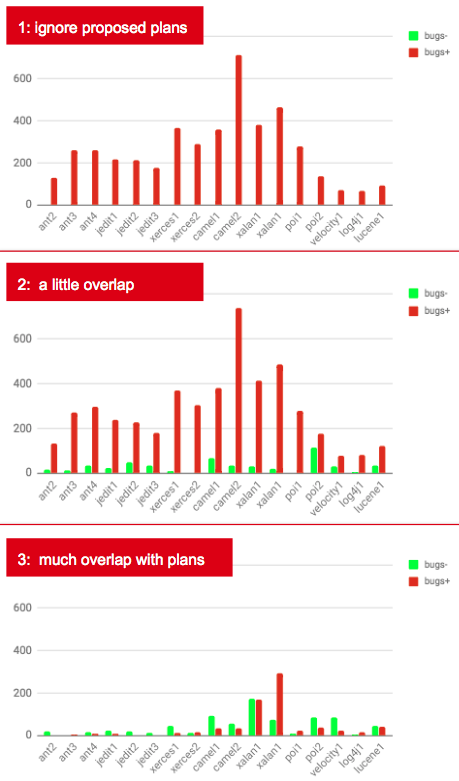
\includegraphics[width=2.9in]{figs/belltree.png}\\\hline
 \end{tabular}
 
 \end{minipage}}
 \caption{At left: Generating recommendations from BELLTREES. At right: effect of the recommendations.}\label{fig:xtree}
\end{figure}

\noindent{\bf 2c. Longer stability with ``Bellwethers''} 
If we cannot {\em generalize} 
from all 10,000+ projects, a more achievable goal is to {\em
slow} the pace of conclusion change.
While it may be
a fool's errand  to wait for   globally stable SE
conclusions, we could declare some  projects as    {\em ``bellwethers''}\footnote{ According to the Oxford English Dictionary, the
``bellwether'' is the leading sheep of a flock, with a bell on its neck.} that make conclusions 
within {\em communities} of related projects.
We  distinguish between the bellwether {\em effect}
and {\em  method}:
\bi
\item \textit{The bellwether effect} states that when a community works on 
multiple software projects, then  there exists one exemplary project, called the bellwether,
which can define   predictors for the others.
\item In the \textit{bellwether method}, we search for the exemplar bellwether project and construct a transfer learner with it. This transfer learner is then used to predict for effects in future data for that community.
\ei
 Note that conclusions are stable
for as long as this bellwether continues to be the best oracle for a community. 
When discussing bellwether methods with colleagues, they often ask:
\bi
\item
{\em Question~1: ``Do bellwethers guarantee permanent conclusion stability?''} No- and we should not expect them to. The aim of bellwethers is to {\em slow}, but do not  {\em stop}, the pace of new ideas in software engineering. Sometimes, new ideas are essential. Software engineering is a very dynamic field with a high churn in techniques, platforms, developers and tasks. In  dynamic environments it is important to change with the times. That said, changing {\em more} than necessary is not desirable- hence, bellwethers. 
\item
{\em Question~2: `` How to detect when bellwethers need updating?''} 
Clearly, the conclusion stability offered by bellwethers only lasts as long as the bellwether remains useful. Hence, bellwether performance must always be monitored and, if that performance starts to dip, then seek a new bellwether. Later in this proposal, we will propose monitoring our models using {\em stream mining}. 
\ei
%\tab{faq} discusses  common questions about Bellwethers.
The experience to date (as reported in ASE'16 and TSE'18~\cite{KrishnaMF16,krishna2018bellwethers}) is that 
bellwether methods are (a)~{\em simple to implement},
(b)~{\em general and useful} in many SE domain;
 (c)~generates succinct and {\em effective actionable analytics};
(d)~{\em comparable, or better,
than   other 
transfer learning methods}:

~{\em (a.) Simple to Implement:} Given a community
of $N$ related projects, a bellwether method 
merely wraps a for-loop around some learner that
trains on project $N_i$ then tests on all other projects $N-N_i$. The project $N_i$ that generates the best performance is then designated as the bellwether. 
% Note that if the communities
% are unknown, then this search must execute with a $O(2^N)$ search through all subsets of the data.
% (later in this proposal, methods are discussed to significantly reduce the cost of this  $O(2^N)$ search to $O(N)$). 


~{\em (b.) General and useful:} 
\fig{xtree} and \fig{motivating_example} presents
a  simple and detailed example of using bellwethers for  planning changes to reduce
future defects.  While that example is about defect prediction,
it is important to note that  bellwethers have been
found useful in many other SE domains as well such as  (1)~predicting defects from static code measures; (2)~identifying bad smells; and (3)~the above Github issue close time problem~\cite{KrishnaMF16,krishna2018bellwethers}. In those tests,  predictions from the bellwethers proved to be as good, as better, than those obtained otherwise. Bellwethers have also been   applied  to (4)~learning effort estimates (where  some slice of a project's prior history were found  useful for predicting  current conditions~\cite{mensah2017investigating,mensah2017stratification,mensah18z}).



 

 
 %XXXheterogenous
\definecolor{ao(english)}{rgb}{0.0, 0.5, 0.0}
~{\em (c.) Succinct and effective actionable analytics:}
\fig{xtree}a shows BELLTREE, a learner 
that
proposes changes to improve software quality.  When used as
the learner within a bellwether method, BELLTREE
finds a project that becomes the
oracle of what to change in other projects.
As shown in \fig{xtree}b,
these changes are very effective
(and see   \fig{motivating_example} for an example of how to apply BELLTREE's recommendations).
When compared to other oracles of ``what to change'', BELLTREEs typically recommends
one to five changes-- which is a three times fewer
changes that recommend by other   ``what to change''
oracles proposed by  Alves, Erni, Hermans, and Shatnawi et al.~\cite{Al10},~\cite{Er96},~\cite{He15}, and~\cite{Sh10}.
Note that such brevity makes BELLTREEs an excellent methods for  generating the tiny models that uses can inspect
in order to improve   their {\em trust} and {\em insight} that they are understanding their project.



\begin{figure}
{ \footnotesize
\begin{minipage}{3in}
{\bf  \fig{motivating_example}a}. Example BELLTRREE recommendations.
`$+$=\textit{increase} and  `$-$',`$\cdot$'=\textit{no-change}.

\resizebox{\linewidth}{!}{\begin{tabular}{ccccccccc}
\hline
\rowcolor{Gray} DIT & NOC & CBO & RFC & FOUT & WMC & NOM & LOC & LCOM \\
$\cdot$ & $\cdot$    & $\cdot$    & $+$   & $\cdot$     & $+$   & $+$   & $+$   & $+$    \\\hline
\end{tabular} }

~\\~\\~\\

{\bf \fig{motivating_example}b.} A sample of possible actions developers can take.
 Here a `$+$' represents an \textit{increase}, a `$-$' represents a \textit{decrease}, and an empty cell represents \textit{no-change}.
Taken from~\cite{stroggylos2007, du2006study, kataoka2002, bryton2009,elish2011,elish2012}. The action highlighted in \colorbox{lightgray}{gray} shows an  action matching BELLTREE's   recommendation. 

\resizebox{\linewidth}{!}{\begin{tabular}{lccccccccc}
\hline
\rowcolor{Gray}Action                                      & DIT & NOC & CBO & RFC & FOUT & WMC & NOM & LOC & LCOM \\ 
Extract Class                               &     &     & $+$   & $-$   & $+$    & $-$   & $-$   & $-$   & $-$    \\
\rowcolor{lightgray} Extract Method                              &     &     &     & $+$   &      & $+$   & $+$   & $+$   & $+$    \\
Hide Method                                 &     &     &     &     &      &     &     &     &      \\
Inline Method                               &     &     &     & $-$   &      & $-$   & $-$   & $-$   & $-$    \\
Inline Temp                                 &     &     &     &     &      &     &     & $-$   &      \\
Remove Setting Method                       &     &     &     & $-$   &      & $-$   & $-$   & $-$   & $-$    \\
Replace Assignment                          &     &     &     &     &      &     &     & $-$   &      \\
Replace Magic Number                        &     &     &     &     &      &     &     & $+$   &      \\
Consolidate Conditional                     &     &     &     & $+$   &      & $+$   & $+$   & $-$   & $+$    \\
Reverse Conditional                         &     &     &     &     &      &     &     &     &      \\
Encapsulate Field                           &     &     &     &     &      & $+$   & $+$   & $+$   & $+$    \\
Inline Class                                &     &     & $-$   & $+$   & $-$    & $+$   & $+$   & $+$   & $+$    \\ \hline
\end{tabular}}

\end{minipage}~~~~~~~~~~~\begin{minipage}{3.5in}
{\bf \fig{motivating_example}c.}

Before ``extract method''. ~~~~~~~~~~~~~~~  After `extract method''.

~\\

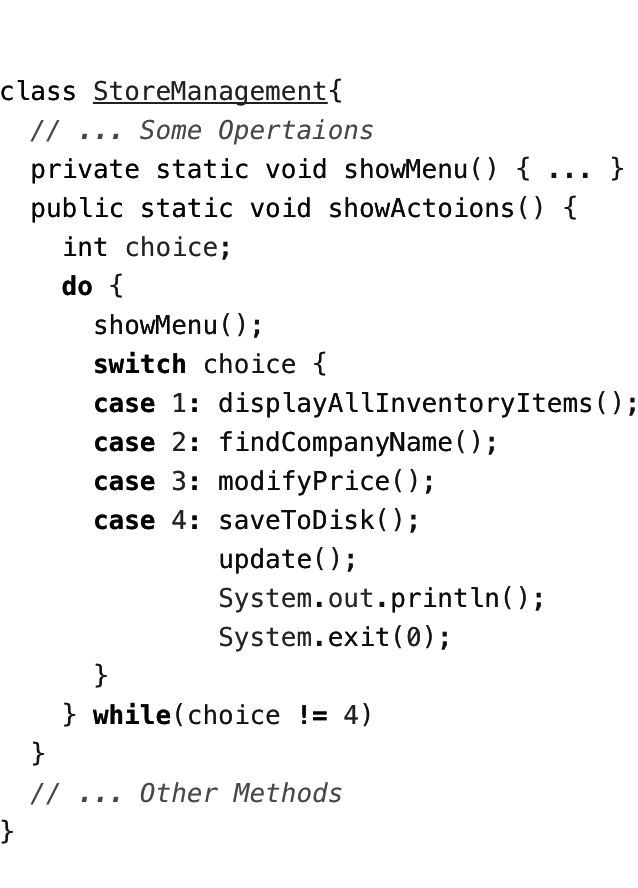
\includegraphics[width=0.5\linewidth]{figs/1.png}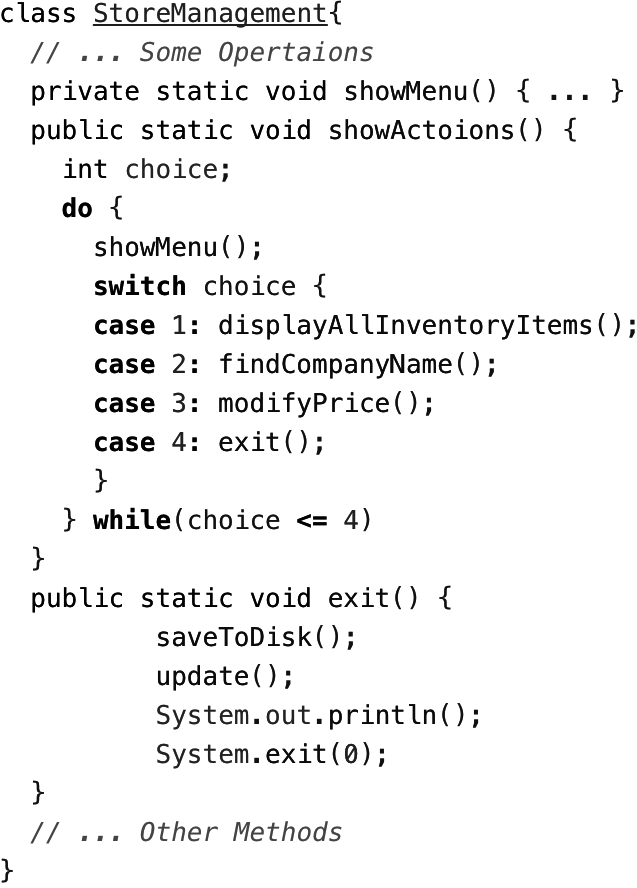
\includegraphics[width=0.5\linewidth]{figs/2.png}
\end{minipage}
}
\caption{ How to  operationalize BELLTREE's advice on ``what to change''. 
METHOD1: Nayrolles et al.~\cite{nayrolles2018clever} 
look through a
developer's own history to find old examples where they have made the kinds of changes recommended by the plan. 
METHOD2: When that data is not available, we use  research papers that
discussed how code changes adjust
static code metrics~\cite{stroggylos2007, du2006study, kataoka2002, bryton2009, elish2011, elish2012}.
For example,  if BELLTREE   recommends the changes of \fig{motivating_example}a, then, we use \fig{motivating_example}b  to look-up possible actions;
e.g.   ``extract method'' best matches BELLTREE's recommendation.  \fig{motivating_example}c shows code before and after
such changes are applied.}\label{fig:motivating_example}
\end{figure}


~{\em (d.) Comparable, or better, than   other 
transfer learning methods:} 
While
the example of \fig{xtree} is based on static code
metrics and defect reduction, the BELLTREE bellwether method is
quite general and has  been
applied to the Github issue close time 
problem of \tab{results} as well
as effort estimation and recognizing code bad smells~\cite{krishna19a}.
For these
domains, the bellwether method has been  compared
to state-of-the-art transfer learning methods:
Transfer Component Analysis (referred to henceforth as TCA+)~\cite{XXX};
Transfer Naive Bayes~\cite{XXX}; and
 Value Cognitive Boosting Learner~\cite{XXX}.
 In that comparison,
 it was observed that
there was no universal best transfer learner that works across multiple domains. That said, simpler baseline methods like bellwethers show comparable performances in several domains. Hence, we recommend bellwethers for all domain, at
least as a first-pass baseline system.


\head{3. RESEARCH QUESTIONS} Before we can scale these bellwether methods to 10,000+ projects, numerous research questions have
to be answered. These questions divide into (a)~overall questions; (b)~systems questions; (c)~technology questions and (d)~evaluation questions: 


\noindent{\bf 3a. The Overall Question}  


{\em RQ1: Is   worthwhile buiding models from 10,000+ projects?}  Can transfer learning (with bellwethers) between 10,000+ project generate better, more insightful, models than
 methods that  just react to  new data sets? Or is learning from so much data inherently so confusing that no general model can be found?
 
The problem of ``too much data confuses model generation'' can be partially 
mitigated by bellwethers and communities.
Bellwether methods do not try to generalize across all data-- rather, they seek generalizations with in a community of related projects. For a discussion on automatic methods to find those communities in 10,000+ projects, see later in this grant.

That said, even when restricted to communities,
recent research results from the field of medicine suggest
that  attempting to build general models from large amounts of
data   might be inherently misguided. Decades of research on evidence-based reasoning in medicine have not resulted in multiple
stable models of medical knowledge that are widely used by practitioners~\cite{gallego2013role,gallego2015bringing}.  The experience there
is that large scale data collection is slow to conduct,
difficult to aggregate, and the   results become out-dated  when  new treatments and conditions arise~\cite{gallego2013role}. 
Further, studies that   generalize over many patients,
may be irrelevant, given   the particulars of any specific single patient. 

Hence,   within the evidence-based community,
there are now rebel researchers who argue against large scale clinical
trials and literature meta analysis. Instead they prefer
{\em instance-based method} where every new test case results in a new query over the data~\cite{gallego2015bringing}.
Instance-based method return treatment records from  similar patients with similar problems.
Doctors can design treatments for the current patient by reflecting on what treatments
did/ did not work within those records.

It is insightful to contrast this approach with the bellwether method discussed above.
The bellwether methods of \fig{xtree} are a {\em model-based method} where some model
is generated from training data, then that model is applied to test data.
As discussed above, the above bellwether methods produce models that are stable within a community.
 Instance-based methods, on the other hand, are highly  unstable since they change whenever a new test case is processed. 
Hence, if assessed by the criteria of Section~2b, such instance-based  studies have many drawbacks 
relating to {\em generality, trust, insight, training}, and {\em tool development}. 

Nevertheless, if the instance-based
 methods out-perform   model-based methods, then we must (reluctantly) conclude that the best way to reason over 10,000+ projects is to add
all   data into one data bucket, then search it for cohorts to specific projects.
But before we can comparatively evaluate (a)~instance-based cohort methods versus 
(b)~model-based bellwether methods, we have to first resolve   other  
questions. 

\noindent{\bf 3b. Systems Questions}  
 
{\em RQ2: Can we find data on 10,000+ projects?} As discussed
above, we foresee no problems with accessing this amount of data.

\begin{wraptable}{r}{2.2in}
{\small
\begin{tabular}{p{2.1in}} 
\rowcolor{gray!20}\begin{itemize}[leftmargin=*]
\item
No. of Commits $> 20$;
\item
No. of Issues $> 10$;
\item
\# programmers $> 8$;
\item
SW development only 
\item Duration $> 50$ weeks;
\item
No. of Releases $> 0$; 
\item
Collaboration (\# pull requests) $> 0$
\end{itemize} 
\end{tabular}}
\caption{These sanity checks  reduce the number of
Github projects from $10^7$ to $10^4$.
From~\cite{5,21,29}.}\label{tbl:sanity}
\end{wraptable} 
~{\em RQ3: Can we store and query that much information?}
Storing and process all (say) Github's data would be a daunting
systems-level task.  Fortunately, much of that data comes from   ``toy'' projects. Accordingly the research community has adopted a sets of standard ``sanity'' checks
of \tbl{sanity} that  select the projects worth reporting~\cite{5,21,29}.  
Two important aspects of theses checks are that
(a)~they can be performed using Github's API without
first downloading the projects; (b)~only one-in-a-thousand projects satisfy these sanity
checks. Hence we can handle the storage requirements
for this project with standard desktop hardware, plus a few  hard drives\footnote{We estimate that storing relevant Github data from 10,000 projects will required 4-5 terabytes (a number small enough to be handled by standard desktop hardware and a few extra hard drives).} \footnote{There are other
important tricks required to download numerous projects from Github. That site limits the number of accesses to 5000 per hour per user token. In the past, we have created ``token pools'' from all researchers in our lab to increase that to 50,000 per hour.
Another important trick is to temporarily
``throttle back'' queries every hour or so 
in order that the Github website demons do not incorrectly
block us as a denial of service attack}.


% [5]ChristianBird,PeterCRigby,EarlTBarr,DavidJHamilton,DanielMGerman, and Prem Devanbu. 2009. The promises and perils of mining git. In Mining Software Repositories, 2009. MSR’09. 6th IEEE International Working Conference on. IEEE, 1–10.

% [21]Eirini Kalliamvakou, Georgios Gousios, Kelly Blincoe, Leif Singer, Daniel M German, and Daniela Damian. 2014. The promises and perils of mining github. In Proceedings of the 11th working conference on mining software repositories. ACM, 92–101.

% [29]NuthanMunaiah,StevenKroh,CraigCabrey,andMeiyappanNagappan.2017. Curating GitHub for engineered software projects. Empirical Software Engineering (2017), 1–35. https://doi.org/10.1007/s10664-017-9512-6




\begin{table*}[!t]

\caption{Featues that can be extracted from 10,000+ projects.
Following  Fenton's~\cite{Fe14} guidance,  attributes are categorized into product, process, and resource. Note that {\em internal}
metrics can be measured directly and {\em external} ones
represent the indirect external manifestations of the internal ones.  }
\label{tab:metrics}
\centering
\resizebox{1\linewidth}{!}{
\begingroup\setlength{\fboxsep}{2pt}
\colorbox{lgray}{%
\scriptsize
\begin{tabular}{r|ll}
\textbf{CATEGORIES}  & \multicolumn{1}{c}{\textit{\textbf{Internal attributes}}} & \multicolumn{1}{c}{\textit{\textbf{External attributes}}} \\ \hline
 \textit{\textbf{Products}} & \\ 
\multirow{2}{*}{Specifications} & \multirow{2}{*}{\begin{tabular}[c]{@{}l@{}}size, reuse, modularity, redundancy, \\ functionality, syntactic correctness, \dots\end{tabular}} & \multirow{2}{*}{comprehensibility, maintainability, \dots} \\
 &  &  \\
\multirow{2}{*}{Designs} & \multirow{2}{*}{\begin{tabular}[c]{@{}l@{}}size, reuse, modularity, coupling, \\ cohesiveness, inheritance, functionality, \dots\end{tabular}} & \multirow{2}{*}{quality, complexity, maintainability, \dots} \\
 &  &  \\
\multirow{2}{*}{Code} & \multirow{2}{*}{\begin{tabular}[c]{@{}l@{}}CK metrics, McCabe metrics, Halstead metrics,  \\ functionality, algorithmic complexity, control-flow structuredness, \dots\end{tabular}} & \multirow{2}{*}{\begin{tabular}[c]{@{}l@{}}reliability, usability, maintainability, \\ reusability\end{tabular}} \\
 &  &  \\
Test Data & size, coverage level, range of change of all the above \dots & quality, reusability, \dots \\
Etc & \dots & \dots \\  \hline
\textit{\textbf{Processes}} &  &  \\ 
\multirow{2}{*}{\begin{tabular}[c]{@{}l@{}}Construction\\ specification\end{tabular}} & \multirow{2}{*}{\begin{tabular}[c]{@{}l@{}}time, effort, \#requirement changes,\dots  \end{tabular}} & \multirow{2}{*}{quality, cost, stability, \dots} \\
 &  &  \\
\multirow{2}{*}{Detailed design} & \multirow{2}{*}{\begin{tabular}[c]{@{}l@{}}time, effort, number of specification faults found, \dots\end{tabular}} & \multirow{2}{*}{cost, cost-effectiveness, \dots} \\
 &  &  \\
Testing & time, effort, number of coding faults found, \dots & cost, cost-effectiveness, stability, \dots \\
Maintenance & \#bug reports, \#maintenance requests, \#enhancement requests,\ldots & extensibleness\dots\\
            & \#issues open, \#issues closes, \#issue close time  \dots &   maintainability \dots \\
Etc & \dots & \dots \\   \hline
\textit{\textbf{Resources}} &  &  \\
%Personnel & age, price, \dots & productivity, experience, intelligence, \dots \\
Teams & size, communication level, structuredness, \dots & productivity, quality, \dots \\
Organizations & size, pace of personnel change %ISO Certification, CMM level 
& Maturity, profitability, \dots \\
Software &   size, \dots & usability, reliability, \dots \\
%Hardware & price, speed, memory size, \dots & reliability, \dots \\
%Office & size, temperature, light, \dots & comfort, quality, \dots \\
Etc & \dots & \dots \\ 
\end{tabular}}
\endgroup}
\end{table*}

As to what specific data we would explore, that is determined by the tasks described above:
\bi
\item {\em Task1:} issue close time;
\item  {\em Task2:} hero alerts (patterns of overcomits);
\item {\em Task3:} Impact of different developer skills on software projects;
\item {\em Task4:} Test case prioritization;
\item  {\em Task5:} Unsupervised learning;
\item  {\em Task6:} Defect prediction;
\item  {\em Task7:} Next-month effort estimates;
\item  {\em Task8:} Overall effort estimation;
\item  {\em Task9:} Change planning.
\ei
Since they above tasks are  well-explored in the literature, we can (a)~use pre-existing experimental methods and evaluation criteria; and (b)~use  baseline results  from the literature to 
assess   our new methods. 
One reason to use these tasks is that 
they cover a range of data types including (a) unstructured textual artifacts;  (b) metrics about human process and experience; (c) process metrics; as well as (d) traditional static code measures.
Another reason to explore these tasks is that 
they address
issues raised by two recent surveys in the SE analytics community
about  `questions that matter in SE''~\cite{Begel:2014,gupta2015identifying}.
For example, XXXX







~\noindent{\em RQ4: Can we ensure data quality over so many projects?} Consider the old adage: ``garbage in, garbage our`` . In the context of this proposal, this quote is 
very pertinent. There are many ways to make mistakes when learning from 10,000+ projects
(e.g. see some examples  in \tbl{ohshit}).
\begin{table}[!t]
\caption{A small sample of the kinds of errors novices make when processing larage data dumps from Github. This list is hardly complete and researchers exploring large Github data dumps need to maintain and extend their own list of ``bad smell'' detectors showing what errors were made before, and how to avoid them in the future. }\label{tbl:ohshit}
\begin{tabular}{p{.95\linewidth}} 
\rowcolor{gray!20}
{\small \begin{itemize} 
\item
Using projects that violate the sanity checks of \tbl{sanity}.
\item
Not noticing rows with identical values;
\item
Not noticing  data cells with impossibly
large values;
\item
Forgetting to process the non-master branches;
\item
Incorrectly aggregating the data. Certain Github labels have different meanings to different developers. E.g. {\em high severity} can actually mean ``the thing I am most willing to fix next''.
\item
Applying a classification learner to data sets with numeric classes;
\item
Applying a learner that assumes discrete data (e.g. APRIORI).
to columns of numeric data; 
\item
Applying the training and test procedures  to the same data
(which grossly can {\em over-estimate} the performance of that learner on future data).
\end{itemize}} 
\end{tabular}
\end{table}
How avoid such errors? Also,  if such mistakes are detected, how to
ensure they are not ever made again?
Manually checking all data from 10,000+ projects  is impossible
so we will  adopt a policy of 
\bi
\item
Stochastic spot checks; and 
\item
Libraries of bad smell detectors.
\ei
Stochastic spot checks is the process of pausing the normal
work flow and manually inspecting a (very small) randomly selected part of the data  generate from Github. The point of these spot checks is  reaching the  ``hmmm... that's funny'' moment where the engineering finds some ``bad smell'' in the data (see \tbl{ohshit}).  Finding ``bad smells'' should prompt
(a)~bug
fixes to the data pre-processing scripts;  (b)~recollection of the damages data;
(c)~the creation of an  bad smell ``demon'' that checks for this  error  in all
future processing.

Depending on the nature of the bad smell, some of these demons can be automated (e.g. using natural language sentiment analysis to recognize
the actual bug reports~\cite{someReference}) while some of them are manual
(e.g. during code inspections, run over a checklist of common errors). 
However they are implemented, they can be used
to collect some insightful  statistics.
By tracking their rate
of creation and triggering, we can gauge our success at handling the the systems problems associated with processing 10,000+ projects. Specifically, we would hope that month-to-month in a  mature
processing environment of 10,000+ projects:
\bi
\item
 Demons are created and are triggered at a {\em decreasing} frequency;
 \item
 Meanwhile, the learning results in this environment are achieving {\em increasing}
 levels of performance.
 \ei

 

 

\noindent{\bf 3c. Technology Questions}
Note that, strictly  speaking, the above   systems questions  are not research issues-- but they are important matters   that must be addressed before exploring
our {\em technology questions}.


~{\em RQ5: How to Finding Communities?} In the above studies, determining the {\em community} of related projects for the bellwether methods was performed manually by   subject matter experts. Scaling bellwethers to 10,000+ projects will need  clustering methods for finding  communities. Once such clusters are known then all subsequent reasoning can be constrained to just within individual clusters.

There are many ways to cluster software data.
One way is via {\em artifact type clustering}; i.e assume that similar projects produce similar artifacts. For example, we might separate our projects that have class-level data  versus those that do not.
It might even be useful to cluster based on main development language (so cluster C++ projects separate to Java projects).

While artifact type clustering is simple, our expectation that is that it would be insufficient to capture all the nuances of 10,000+ projects.
Hence, we need to augment artifact type clustering with other methods. 

One other method  is to use 
{\em manual stratifications} e.g. as discussed on page one of this proposal,
Petersen and Wohlin~\cite{petersen} divides software into 100s of groups according to their different types of product, process, practices, people, development organizations, and target markets. While we agree
with their central intuition (that there many different kinds of projects that deserve different models), they present no evidence that their manual stratifications are ``best'' in some manner.
For example, 
Clark and Madachy~\cite{clark15} divided their software projects in a very manner to
that of  Petersen and Wohlin~\cite{petersen}.

In our research, we have found that models learned from automatic clustering methods
perform better than those from manual stratifications~\cite{meTSE06,meTSE12lcoalglobal}.
Hence, we will eschew manual stratifications and explore automatic clustering methods
using a vector space representation (VSR) of the data.
Given $F$ features extracted by joining across Github data, we would create tables of data, one per project. Each row of those tables is a vector describing  one specific artifact with the projects (e.g. a function, a class, or a file). For this proposal, clustering means find similar projects; i.e. those with similar vectors.


In prior work,
we have had much success with
   clustering software data using techniques 
such as k-means~\cite{suvodeepMSR18} or 
 the pseudo-labelling method of He et al.~\cite{hemenziesESEM13}.  In the latter, data from different projects are labeled P1,P2, etc and for each pair $P_i,P_j$ a classifier is built.
The accuracy of this classifier is a measure of the distance between  $P_i,P_j$  (the larger
the error, the more similar and hence the closer the projects).   These distances could then be used by some other clustering methods. 

Note that all the above require $O(N^2)$ comparisons of pairs of projects.
Other clustering methods approach $O(2N)$. For example,
  {\em spectral clustering}  can use a linear-time method called FASTMAP to recursively bi-cluster the data\footnote{Step1: pick any vector $X$ at random.
  Step2: pick the vector $Y$ most distant to $X$. Step3: pick
  the vector $Z$ most distant to $Y$.
  Faloutsos et al. note that step1 takes virtually no time while
  steps 2 and 3 take 
  time linear on the number of vectors~\cite{faloutsos1995fastmap}.}.
  At each level of the recursion, two distant ``pole'' points are found in time $O(2N)$ and data separates according to which ``pole' is closer.
  
There exist other, even faster, clustering algorithms
including canopy clustering~\cite{McCallum:2000}, hierarchical DBSCAN~\cite{campello2015hierarchical}, and a 
  $O(N)$ method called {\em  locality-sensitivity hashing}~\cite{Andoni:2015}.
Starting with  $D$ vectors (picked at random), LSH stream over the rest the data and compute the
sign of the cosine distance between each new vector $X$ and all vectors $d\in D$. Generate a reverse index of $2^D$ bins where vectors in each bin  are aligned in the same direction (i.e. they are share the same cosine signs).  Building this index takes time $O(DN)$ which is negligible  for small values of
$D$ (e.g. $D=10$). To use this index, perform  any of the above indexing methods, but only for the vectors in the same or nearby bins. Assuming $D=10$, this would divide the clustering into $2^{10}> 1,000$ smaller sub-problems. 


As seen in this section, 
there are many ways we might find the communities (and some of those methods are very fast indeed). As to which is most useful, that would require experimentation to find the best cluster method (and the best clustering method would be the one that generates data clusters which, once studied by machine learners, produce models with highest predictive prowess).


 

~{\em  RQ6: How to Scale?} The bellwether method's search for  has to be optimized
before we dare try to scale the bellwether method to 10,000+ projects. This search cost has two components: (a)~find the communities then (b)~search within those communities for the bellwether. A naive search for the  communities that explores all subsets of projects
  takes time $O(2^P)$   and   $O(lc^2)$,  respectively, where $P$ are the number of projects; $c$ is the size of the community and $l$ is the cost
  of running the learner across the pairs of projects within a community.
  For $P>10,000$, this naive approach is clearly impractical.

As mentioned above, there are clustering methods that can reduce
 $O(2^P)$  to $O(P)$. For example, with  locality sensitivity hashing, we could ignore projects
 that do  not fall to the similar bins.
 
 As to the second cost, the $c^2$ comparisons seem fundamental to the bellwether method, so we need to focus on reducing the learning cost $l$.
There are many ways we might do this.
Firstly, we could use instance selection methods~\cite{song2017efficient} to reduce the size of the data presented to the learners.
Such instance selectors find {\em prototypes} where are exemplar vectors that can ``stand-in'' for dozens of other 
vectors. For example, we could apply locality sensitive hashing recursively within each bin and  then just keep
a few vectors per bin. Alternatively, we could use Peters' linear time LeaF algorithm algorithm~\cite{petersLace2Icse15} 
that builds an an anomaly detector from a small number of vectors, then streams over the rest
of the data, marking as ``interesting'' any other is is anomalous (i.e. that kind of vector has not been seen before).
In practice, LeaF marks just  5-20\% of the vectors as ``interesting'' and worthy of subsequent exploration with a learner. 




Secondly, we could use faster learners. Ghotra et al.~\cite{Gh15} 
show that of the performance scores of  dozens of learners commonly used in software analytics divide into just a few groups.
Hence, we could experiment with finding bellwethers using
the fastest method within the top group (e.g. simple logistic regression).

Note that finding the right way to scale this approach would require experimentation. The right scaling method
would run quickly enough to handle the volume of data we expect~\footnote{rahul: how many vectors in total}  while
not degrading the performance of the transfer learners (for learner performance measures, see RQ7, below).

% {\em  RQ6: How to transfer lessons learned between projects described in different terminology?} 
% When transferring data between many projects, there is sometimes a need for
%  heterogeneous transfer learning~\cite{nam2017heterogeneous}; e.g.  realizing that that feature  ``X'' in project1 is effectively the same as feature ``Y'' in project2. Learning such {\em heterogenous transforms} is problematic for 10,000+ projects. To address this problem, this research will  constrain heterogeneous transfer  to just the attributes mentioned in BELLTREE's recommendations (which, as mentioned above, make use of very few features).  

~{\em RQ7: How to tame tuning complexity?} As software analytics gets more complex (e.g. deep learning~\cite{weFSE17}, spectral learning~\cite{vivekEMSE}), it becomes
harder and slower to test many methods on many data sets.
Worse yet, many recent results have demonstrated the value of tuning
a learners default parameters~\cite{agrawal17,agrawal2018wrong,Tantithamthavorn18,fu2016tuning} before apply those learners to software engineering data.
That is, in the near future, it will be required standard scientific
practice to tune learners before any results can be reported from that study.

 
The problem with tuning is that it is expensive.
Using 
some
standard genetic algorithm as the optimizer,  learners might be called tens of thousands
of evaluations (or more)  to evaluate different settings~\cite{menzies18}.  Recently
we have had much success with faster methods for hyperparamter optimization, the best of which is Nair \& Menzies' work on the FLASH Bayesian Parameter Optimization algoritthm~\cite{nair18tse}. 


\begin{wrapfigure}{r}{1.4in}
    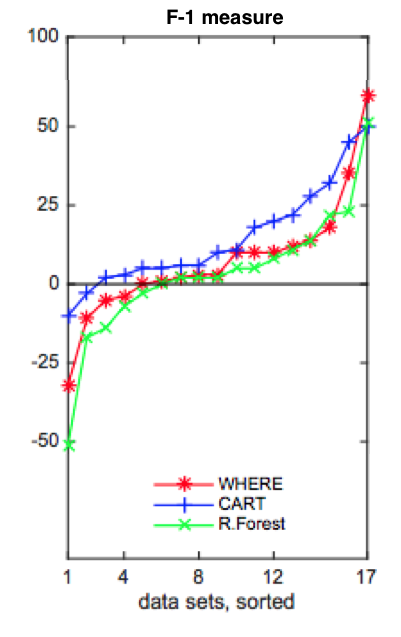
\includegraphics[width=1.4in]{figs/f1.png}  \caption{Performance improvements seen in 17 defect prediction data sets after   hyper-parameter optimization.}\label{fig:tuned}
\end{wrapfigure}Recently, the PIs of this proposal have had much success  with   ``hyper-
parameter optimizatiers'' that automatically determine which learner to use, and what settings to apply to those learners~\cite{fu2016tuning,chen2017riot,nair2017flash,agrawal2017better,agrawal2017better,fu2017revisiting,nair2017using,mathew2017shorter,nair2017faster,chen2017beyond,nair2016accidental,fu2016differential,chen2016sampling,agrawal2016wrong,agrawal2018better}.
As seen in  Figure~\ref{fig:tuned}, this can   significantly improve learner performance. That figure shows the  improvements found by Fu and PI Menzies
can after a hyperparameter optimizer adjusted the control
 parameters of data miners~\cite{fu2016tuning}. The x-axis of that figure shows results from 17 different data sets. The y-axis shows the delta 
\mbox{{\em after - before}} seen in three different
learners: CART, Random Forest, and WHERE.
Note that in half those data sets, hyper-parameter optimization
resulted in positive, and sometimes very large improvements.

This proposal will explore Sequential Model-Based Optimization~\cite{Bergstra:2011} for both speeding up learnes and speeding
up hyperparamter optimization.
SMO  incrementally explores the control parameters of a data miner as follows.
\begin{enumerate}
\item Set a budget $b$ for maximum number of evaluations.
\item
Run the data miner using $n$ randomly selected control parameters.
\item Build an {\em archive} of  $n$   examples holding pairs of  parameter settings and   their resulting performance scores
(e.g. precision, recall, etc).
\item
Using that archive, learn a {\em surrogate}   to predicts performance;
\item Use the surrogate to guess  performance scores of 
$N \gg n$ parameter settings.
\item Using some {\em selection  function}, select  the most ``interesting'' setting. 
\item Collect performance scores by applying    ``interesting'' to the data miners. 
\item  Add  ``interesting'' to the archive. Set $n=n+1$. If $b>n$, goto step 3.
\end{enumerate}
In our own SMO  experiments with defect prediction and configuring video encoding software, we have used $b=50,n=20, N=1000$, and the CART
decision tree learner to learn the surrogates~\cite{nair18tse}. Since we were trying to minimize the error in predictions,
our {\em selection function} was to use the example that generated largest predictions.
For learning from 10,000+ projects, SMO has much to recommend it:
\bi
\item
Most of the reasoning is done using the surrogate, which is much faster than actually running the data miners with different settings.

\item
The parameter settings found in this way could be used to assist in the clustering problem described above. In 2013, we showed that it was possible to cluster data based on performance scored earned from data miners; i.e. similar data sets respond well to the same kinds of data miners~\cite{he13}. Hence if run SMO on all projects, then we can constrain clustering to just those projects that have similar learner parameter tunings.
\item
Using {\em reservoir sampling}\cite{Vitter:1985}, 
SMOs can   stream over an infinite stream of data. That is  in step8, at probability $(1/n)^p)$ replace old items in the archive
with new information.  In this way, the memory requirements for processing long temporal streams of data can be reduced. Note that
by using $p<1$, we can learn to favor more recent examples over past examples.
\item
This approach can easily extended to multiple goals as follows: in step4, build one surrogate model for each different goal (we applied that approach, with much success, in a TSE'18 paper~\cite{nair18}). For example, we could tune data miners to {\em maximize}   precision,
{\em maximize} recall,  while at the same time {\em minimize} the size of the generated model
and {\em minimize} learner training time. That is, we could learn how to quickly find succinct, useful models.
Note that this would address the $l$ cost discussed in {\em RQ6}.
\item
Once we can support SMOs and stream mining, we can run over very large temporal samples of SE data to learn when older models need to be replaced with new models. 
\ei


\noindent{\bf 3d. RQ8: How to Evaluate? }

{\em RQ8a: What Performance Scores? }To evaluate the above, we will apply the evaluation criteria defined in papers that explored {\em Task1} to {\em Task9}. That
criteria is many and varied. For example:
\bi
\item
{\em Task2:} Amritanshu et al.~\cite{agrawal17hero}   assess the impact of projects using   ``hero programmers'' (where 80\% of the changes come from 20\% of the developers) via a statistical
comparison between the   
the bug close rate in hero and non-hero projects. 
\item
{\em Task6:} On the other hand, Huang\&Lo et al.~\cite{huang} evaluate their defect predictors   using ``IFA'' which is the number of false alarms seen before finding the first true positive defect.
\ei
In this proposal, for each {\em Task$_i$}, 
we will apply the  evaluation criteria used in recent state-of-the-art software analytics papers relating to {\em Task$_i$}.

That said, across all our tasks, some general principles will apply.
For example, 
to avoids issues with non-Gaussian
distributions, we will check all effects seen in our data using
 non-parametric significance tests and effect size tests. Specifically,
 we will use the Scott-Knot tests championed at TSE'13 by 
 Mittas et al.~\cite{Mittas13} using Efron's bootstrap~\cite{efron93} test of statistical significance and the Cliff's
delta effect size test to check that distributions are actually different. We use Cliff's Delta since that has
recently become a standard test in software analytics~\cite{Gh15}.

After from that, there are number other important evaluation principles for this research:

{\em RQ8b: Beyond Decision Trees?}
The above discussion assumed that models were generated by decision trees learned from bellwethers within a community. That approach has the advantage of generating succinct, easily readable models.  There are any other ways to generate such models (bayes nets~\cite{misirli2014bayesian}, 
rule generation algorithms like RIPPER~\cite{cohen1999simple} and FFTrees~\cite{chen2018applications}; etc) and the best model generation method
must be explored as part of this evaluation task.

{\em RQ8c: Do Models Matters?} as discussed in {\em RQ1}, we need to check if  instance-based queries   over data performs much better
than models generated from bellwethers (like \fig{xtree}b).
If so, then   irregardless of the  issues listed in Section~2b (generality,
trust, insight, training and tool development), we would have to endorse
instance-based methods studies (and their associated conclusion instability).

{\em RQ8d: Is Volume Possible?} We need to test if our methods
can find, then ingest, then process data from  10,000+ projects. We would have to doubt the practicality of that scale up if:
\bi
\item We cannot find enough data (discussed in {\em RQ2}).
\item The disk requirements for our data storage grew too large (discussed in {\em RQ3}); 
\item We cannot tame the  data ingest problem and our
  bad smell detectors (discussed in {\em RQ4})    firing at an {\em increasing} frequency;
\item We cannot find communities (discussed in {\em RQ5}); i.e. the performance of  models learned from  clusters
 is no different to models learned from the entire data.
 \item The inference time (discussed in {\em RQ7}) is too slow (we would seek answers in minute to hours, not days to weeks);
\item Hyper-parameter optimization (discussed in {\em RQ7}) became to burdensome.
For example, standard hyper-parameter optimizers using evolutionary
algorithms required thousands to millions of evaluations~\cite{sarro2016multi}. 
On the other hand,
the SMO methods described in {\em RQ7} terminate after a few dozen evaluations (which is not burdensom). That said, SMO has yet to be    tested on data from 10,000+ projects.

\item The streaming learners  discussed in {\em RQ7} cannot recognize when
old models need to be replaced with new models (which would be witnessed by a steady decline in performance as the reasoning continues across a long stream of data).
\ei
{\em RQ8e: Does Volume Matter?} i.e. does {\em more}
data means {\em better} predictor (where ``better'' is some domain-specific predicate discussed in our first point). To address this question, all our evaluations must be performed on 10000+ projects,
then 5000, 2500, 1250, 600, 300, 150, 80, 40, 20, 10  projects (selected at random).
We would reject the premise of this proposal (that it is useful to learn from 10,000+ projects)
if models learned from (say) 20 projects do just as well as those learned from (say) 2,000.



{\em RQ8f: Does This Work for Future Data?}
it is important to apply our evaluation to both historical  {\em and } new data.
While verification of past data is useful, the real test for our methods is how well
it works on {\em new} data. That is, in order to demonstrate the external validity of our methods, we will watch for new releases of the projects we are studying. When such new releases occur, we will apply our current models to those new releases. This will demonstrate the value (or otherwise) of our models on new data.
 

\head{4. RESEARCH PLAN}
This grant will fund two graduate students (G1, G2) who will work full time on this proposal.
Over our three year grant, these students will work as follows. 

XXXX need rq1 somewhere

\begin{center} 
{\footnotesize \begin{tabular}{r|r|c|c|ccc}\hline
\rowcolor{gray!20}&       &                          & Research & & &\\
\rowcolor{gray!20}Id&What  &                      Who &  Questions    &     Year1 &Year2& Year3\\\hline
1&Collect eval criteria (from the literature)& G1,G2&RQ8 &     \CheckmarkBold\\
\rowcolor{gray!20}2&Data collection&G1 &   RQ2,RQ3,RQ4               &     \CheckmarkBold&&\\
3&Technology construction   &  G2 &   RQ5          &      \CheckmarkBold\\
\rowcolor{gray!20}4&Scale up                  &  G1 &   RQ6         &          &    \CheckmarkBold&\\
5&Hyperparameter optimization& G2 &   RQ7         &          &    \CheckmarkBold\\
\rowcolor{gray!20}6&Evaluation (on old data)   & G1,G2& RQ8         &       \CheckmarkBold  &  \CheckmarkBold  &  \CheckmarkBold\\
7&Evaluation (on new data)   & G1,G2& RQ8          &           &     &  \CheckmarkBold\\
\rowcolor{gray!20}8& Community support         & G1,G2 &          & \CheckmarkBold  &  \CheckmarkBold  &  \CheckmarkBold\\\hline
\end{tabular}}
\end{center}         

\noindent
Note that {\em Evaluation} breaks into two sections:
\bi
\item {\em Evaluation (on old data)} is a task that will be on-going throughout this project;
\item But {\em Evaluation (on new data)} is a task that has to wait till the end (since we will need new data from the projects that we are monitoring)
\ei
All along this plan, research results can be written:
\bi
\item In Year1, we can report on quality operators for ingesting large data set
\item In Year2, we can report or on scale-up methods for large scale analytics;
\item In Year3, we can report (hopefully) on what kinds of models hold for most data;
\item In all years, we can report results where new methods are applied to old data sets (hopefully to generate new and better and more interesting results); 
\ei
As to the last item ({\em Community Support}), 
in all our work, we  publish papers along with reproduction packages containing all the data and scripts needed to replicate
that paper. This work will continue that tradition (for more on this point, see {\bf 7.4. Dissemination of Knowledge}, below).
  In practice, this means that some part of our time will be required for {\em Community Support} to help other research teams boot and run our scripts.

\head{6. RELATED WORK}

Need numbers of this: a quick survey. Yet  a  typical research paper in software analytics studies less than a few dozen projects (exceptions: see [?]).


Boa: mostly for searching abstract syntax tres 

GhTorrent

cmu does mega learning but for specific problems. tthe general issue of the emrits of elarning from so much data is still unknown


% \paragraph{Anti-patterns}

Anti-patterns are poor solutions to recurring design problems. They occur in object-oriented systems when developers unwillingly introduce them while designing and implementing the classes of their systems~\cite{fowler99}. In addition to anecdotal evidence, in the past decade anti-patterns have been empirical shown to have an detrimental impact on software quality~\cite{Ab11, Ar11, Ch10, Kh12, Li07}. There is also very strong evidence that the number of anti-patterns in software systems increases over time and only in few cases are they removed through refactoring operations~\cite{Ar11,Ch10}. Researchers have called for recommendation systems supporting the software engineer in (i) identifying anti-patterns and (ii) designing and applying a refactoring solution to remove them~\cite{Ba98}. Among the 30+ anti-patterns defined in the literature~\cite{fowler99,Ky05}, only for a subset of them we have
approaches and tools for their automatic identification. A survey of literature suggest that most widely used tools such as DECOR~\cite{decor} use a set of rules, called “rule card”, describing the intrinsic characteristics of a module/class affected by anti-patterns. Beside DECOR, other approaches also rely on rules generated by metrics to identify anti-patterns in source code. For example,
Marinescu~\cite{Ma04} presented a detection strategy able to identify anti-patterns by generating rule derived from deviations from good design principles. Fowler \cite{fowler99} and Brown
et al.~\cite{Br98} defined more than 30 anti-patterns. However, in the previous year, researchers concentrate their attention only on a small subset of anti-patterns defined in the literature. Palomba et al.~\cite{Pa15} assert that this limitation is due the difficulty in generating rules for identification of code smells. Methods such as CrossTREE may be particularly useful in these cases. In fact, Krishna et al.~\cite{krishna17a} have already shown that CrossTREE can be used to reason effectively about anti-pattern to assist reorganization efforts to address them. It must be noted that by augmenting CrossTREE with developer insights and knowledge combination methods such as PSO, it may be possible to further assist addressing anti-patern.
%\paragraph{Planning}

Planning  has been a subject of much research in artificial intelligence. Here, planning usually refers to generating a sequence of actions that enables an \textit{agent} to achieve a specific \textit{goal}~\cite{norvig}. This can be achieved by classical search-based problem solving  approaches or logical planning agents. Such planning tasks now play a significant role in a variety of demanding applications, ranging from controlling space vehicles and robots to playing the game of bridge~\cite{ghallab04}. Some common planning paradigms include: 
\be
\item[(a)] \textit{Classical planning:} This is used when the initial state is fully-observable and any action is deterministic. Classical Planning is most useful when the problem is not very complex and there's a well-founded model~\cite{strips,wooldridge95}. In case of complex domains like SE, classical planning is highly inefficient~\cite{ghallab04}; 
\item[(b)] \textit{Probabilistic planning:} Here the outcomes may be random and are partly controlled by the decision maker~\cite{Bel, altman99, guo2009}. These kinds of planning problems are usually solved using dynamic programming and reinforcement learning\cite{ghallab04}; 
\item[(c)] \textit{Preference-based planning:} This is an extension of the above planning schemes with a focus on producing plans that satisfy as many user-defined constraints (preferences) as possible~\cite{son06 , baier09}. 
\ee

Note that the existence of a model precludes the use of each of these planning approaches. This is a limitation of all these planning approaches since not every domain has a reliable model. 

There are at least two kinds of planning research in SE which are distinguishable by {\em what} is being changed. In {\em test-based planning}, some optimization is applied to reduce the number of tests required to achieve to a certain goal~\cite{tallam2006concept, yoo2012regression, blue2013interaction}. In {\em process-based planning} some search-based optimizer is applied to a software process model to infer high-level business plans about software projects. For example, Ruhe et al.'s work on next release planning in requirements engineering~\cite{ruhe2003quantitative, ruhe2010product}. This proposal is about {\em code-based planning} where the goal is to change a code base in order to improve that code in some way. More generally, in software engineering, the planning problem translates to proposing changes to software artifacts. Solving this has been undertaken via the use of some search-based software engineering techniques~\cite{Harman2009}, with algorithms such as SWAY, NSGA-II, etc.~\cite{Nair2016,deb00a}.

These search-based software engineering techniques require access to some trustworthy models that can be used to explore novel solutions. In some software engineering domains there is ready access to such models which can offer assessment of newly generated plans. Examples of such domains within software engineering include automated program repair~\cite{Weimer2009, LeGoues2015}, software product line management~\cite{sayyad13, henard15}, etc. However, not all domains come with ready-to-use models. For example, consider software defect prediction and all the intricate issues that may lead to defects in a product. A model that includes {\em all} those potential issues would be very large and complex. Further, even when there is an existing model, they can require constant  maintenance lest they become out-dated. In such domains, we seek alternate methods for planning that can be automatically updated with new data without a need for comprehensive models. One approach is to use data mining approaches to create a quasi-model of the domain and make of use observable states from this data to generate an estimation of the model. Our preferred tools in this proposal (CrossTREE) takes this approach by constructing decision trees on available data (discussed in \fig{tutorial}). 
%\paragraph{Anti-patterns}

Anti-patterns are poor solutions to recurring design problems. They occur in object-oriented systems when developers unwillingly introduce them while designing and implementing the classes of their systems~\cite{fowler99}. In addition to anecdotal evidence, in the past decade anti-patterns have been empirical shown to have an detrimental impact on software quality~\cite{Ab11, Ar11, Ch10, Kh12, Li07}. There is also very strong evidence that the number of anti-patterns in software systems increases over time and only in few cases are they removed through refactoring operations~\cite{Ar11,Ch10}. Researchers have called for recommendation systems supporting the software engineer in (i) identifying anti-patterns and (ii) designing and applying a refactoring solution to remove them~\cite{Ba98}. Among the 30+ anti-patterns defined in the literature~\cite{fowler99,Ky05}, only for a subset of them we have
approaches and tools for their automatic identification. A survey of literature suggest that most widely used tools such as DECOR~\cite{decor} use a set of rules, called “rule card”, describing the intrinsic characteristics of a module/class affected by anti-patterns. Beside DECOR, other approaches also rely on rules generated by metrics to identify anti-patterns in source code. For example,
Marinescu~\cite{Ma04} presented a detection strategy able to identify anti-patterns by generating rule derived from deviations from good design principles. Fowler \cite{fowler99} and Brown
et al.~\cite{Br98} defined more than 30 anti-patterns. However, in the previous year, researchers concentrate their attention only on a small subset of anti-patterns defined in the literature. Palomba et al.~\cite{Pa15} assert that this limitation is due the difficulty in generating rules for identification of code smells. Methods such as CrossTREE may be particularly useful in these cases. In fact, Krishna et al.~\cite{krishna17a} have already shown that CrossTREE can be used to reason effectively about anti-pattern to assist reorganization efforts to address them. It must be noted that by augmenting CrossTREE with developer insights and knowledge combination methods such as PSO, it may be possible to further assist addressing anti-patern.
% planning, prediction. no one doing planning.

% \head{BACKGROUND:} Much research has   explored how  automatic methods might assist in the discovery and removal of software bugs (see~\tab{methods}).  That work has two limitations. Firstly, it is somewhat incomplete.  Table 1 Much of the work on automatic analysis of software explores   software \textbf{products} (e.g. source code\footnote{There are some examples where  automatic  methods have been applied to process and resource issues; see~\cite{Ca00,Ra13,Lu12,Me07}. However, such examples are very uncommon.
% }). Yet according to Fenton~\cite{Fe00,Fe14}, software projects can be described in terms of their product, process and resources attributes (see~\tab{metrics}).  This is an important point since, in our industrial  experience\footnote{ From 1987 to 1994, PI Menzies worked as an industrial software consultant  expert systems, then object-oriented systems. From 1998 to 2004, PI Menzies served as the NASA Software Research chair and he spent much time talking to software managers about factors that cause late delivery of low quality code.  In 2010, 2011 PI Menzies spent summer at Microsoft Research (Redmond), working with managers of Microsoft projects about how to best apply data miners to their data. Since 2014, Dr Menzies has been working  with LexisNexis and IBM (at Raleigh), applying data mining to their data.}, when experienced software developers discuss how to ``fix'' projects, to fix  ``bugs''  in a software project, they propose changes to software products \underline{and} processes \underline{and} resources via:

% \bi
% \item Decisions made about  software products; e.g.  how multiple levels of redirection can obfuscate code and make it hard to maintain;
% \item Decisions made about cost/benefit trade-offs made at the process level; e.g. what parts of the project deserve more or less testing;
% \item Decisions made  at the resource level;   e.g.  how many skilled programmers can we take from this project and deploy to other systems that need their help.
% \ei

%  \begin{figure}[ht!]
\centering
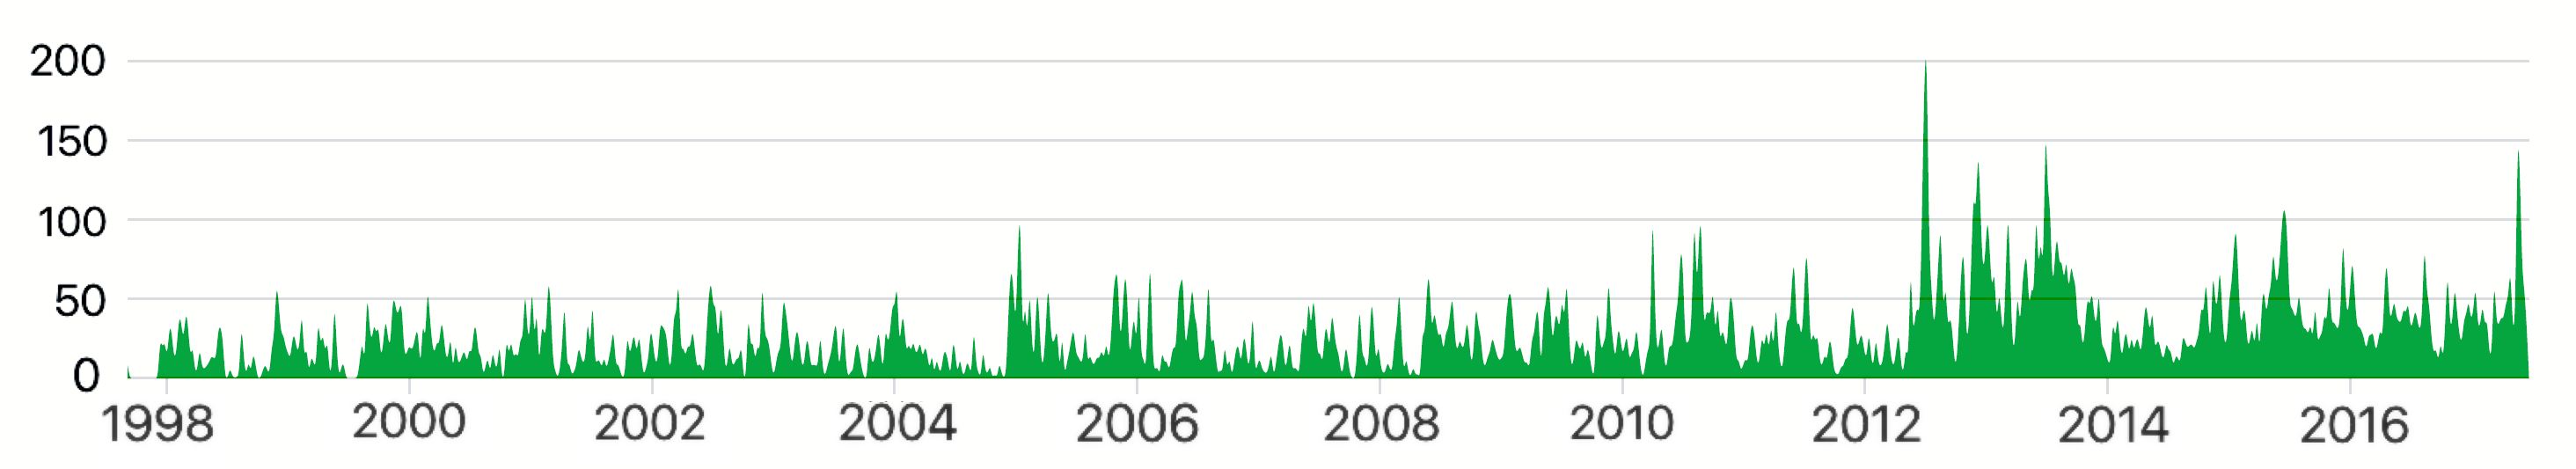
\includegraphics[width=\linewidth]{figs/commits.png}
\caption{This project will use data from many open source scientific programming projects, including the twenty year history available from tools like the deal.II finite elements library. Source: https://github.com/dealii/dealii/graphs/contributors}
\label{fig:commits}
\end{figure}


% \begin{table}[htbp!]
\footnotesize
\centering
\begin{tabular}{|p{\linewidth}|}
\hline
\bi
  \item \textbf{Formal method tools}  such as the SPIN~\cite{Ho11} model checker deploy automatic tools that are guided  quantified formulae which can succinctly express the correct, or incorrect, behavior of a large class of error;
  
  \item \textbf{Static code analyzers} such as Findbugs~\cite{Ay10} scan code looking for issues that might cause defective behavior such as possible logic errors that could lead to null pointer dereferences, bad casts, infinite recursive loops and other problems.  These tools suffer from large false positive reports. 
  
  \item Visser~\cite{Vis14} celebrates recent triumphs in optimizing SAT solvers and their applications to SE quality assurance.  Visser  also warns that automatic tools like SAT solvers are ``blackbox'' and software engineers need to look under the hood to make use of some of the internal results. Further, much work remains in order to fine-tuning such general tools to the specifics of any particular problem.

  \item Researchers in software analytics apply data mining algorithms to  build defect predictors using product attributes~\cite{Ha12} or process attributes~\cite{Ra13} extracted from software code. Foyzur et al. report that the data mining approach can be just as other methods such as effective static code analyzers~\cite{Fa13}.

\ei \\[-0.2cm]
Much prior work has explored the relative cost/benefits of using one or more of the above. For example,   Lowry warns that model checkers have severe scalability problems~\cite{Lo98}.  Also,~\cite{Ow07} comments that   conjunctions of these methods may find more bugs that any single one, but it is hard to predict before hand which, if any, of these methods finds most bugs.  Foyzur et al.~\cite{Fa13} notes that these, these defect prediction methods have fewer bindings to specific languages. This means that (e.g.) when a new version of C\# is realized, vendors of static code analyzers must scramble to adapt their tool to the nuances of the new language. Meanwhile, users of defect predictors can quickly build (in just a few hours) the lightweight parsers required to extract features from the new language.  \\ \hline
\end{tabular}
\caption{\textbf{Automatic methods for addressing code quality.} Since our goal is to monitor thousands of projects implemented in, potentially, dozens of languages, and since Foyzur et al. report that this method is as effective as more complex ones,  this research will take the data mining approach.}
\label{tab:methods}
\end{table}


% The second limitation with the tools of tools Table 1 is that they utilize automatic algorithms rather than  exploiting human domain knowledge.  In this age of the Internet, of social media, of everyone wired and on-line and sharing their ideas all the time, surely we  can augment (perhaps replace) automatic tools with more human expertise.  Previously, it was hard to collect all that human opinion, then assess which parts of that knowledge were useful/useless to some context. However, that is no longer the case. One side effect of more developers working on more open source projects is that many developers now routinely use a similar toolchain; e.g.  Jenkins for testing; Github for code storage/sharing; Jira for  issue tracking; Travis CI for continuous integration, and several other tools as well. \\

% This is a significant point since, once we build feature extractors from Github, Jenkins, Jira, Travis CI, etc, we extract  the  product, process, and resource data discussed above.. For example, since we have access to the source code of these systems (in Github) is it not difficult to extract code metrics. We can also automatically extract  resource and process information such as how often releases are made; how many active developers are part of each team; how long before developers move to different teams; what  developers touch what parts of the code; the time taken to close issues;  etc. Also, we can access quality measures such as reported bug rates, the achieved rate of enhancement within these systems, how many tests fail, how many old issues are re-opened, etc. Working in collaboration with our industrial partners at IBM Raleigh, over several months, we were able to gather data on 1646+ software projects of which 1108 were the most trending opensource projects on github and 538 were proprietary in-house projects. Upon mining these projects, we processed all the projects by running a ``sanity check''. We follow the guidelines of Kalliamvakou et al.~\cite{Ka14} to implement these ``sanity-checks'' which are then used to filter out all the projects.

% \begin{wraptable}[13]{r!}{0.6\textwidth}
\footnotesize
\centering
\caption{Sanity checks. Starting with 1108+538  open source+in-house projects, we discard  projects that {\em fail}
any of the LHS tests to arrive at 661+171 projects.}\label{tab:sanity}
\begin{tabular}{|l|r|r|}
\hline
Sanity check & \multicolumn{2}{c|}{\#discarded projects}                     \\ \cline{2-3} 
\multicolumn{1}{|c|}{(discard projects that violate these tests) }                              & \multicolumn{1}{l|}{In-house} & \multicolumn{1}{l|}{Open-source} \\ \hline
\# Pulls \textgreater 0                             & 35                            & 54                              \\
\# Issues \textgreater 10                            & 60                            & 89                              \\
\# Commits \textgreater 20                          & 68                            & 96                              \\
\# Developers \textgreater 8                        & 47                            & 67                              \\
\# Releases \textgreater 0                          & 136                           & 44                              \\
Project time frame \textgreater 1 year              & 12                            & 46                              \\
Projects doing only software development            & 9                             & 51                              \\ \hline
%Total Projects                                      & 538                           & 1108                            \\
Surviving projects                                  & 171                           & 661                             \\ \hline
\end{tabular}
\end{wraptable}


% \bi
% \item From the scientific programming arena, we can access detailed information about complex software. For example, see~\fig{commits} for 20 years of history about the deal.II finite elements software package. There are many other such scientific software projects that store their project data, on-line and readily available, in a similar manner\footnote{Dozens of such projects were presented at the recent 2017 PI meeting of the nsf  Software Infrastructure for Sustained Innovation (SI\textsuperscript{2}) https://github.com/si2-pi-community.github.io/2017-meeting/}. 

 

% \item Further, from the open source, we can explore a further 1108 open source projects.~\fig{projects} shows  details on some of the most widely known projects. We perform a sanity check to filter out projects that do not have sufficient data to perform the necessary analytics. Out of the 1108 projects, 661 passed our sanity checks (see~\tab{sanity}). 
% \ei

% % But a more important question is how to use all this data to achieve the goals of this research? I.e. how to use all this information to collect, summarize, audit and operationalize the expertise of seasoned software developers?  We can see three approaches. To answer, these questions, we must turn to cognitive psychology and some decades-old results from the field of knowledge acquisition. That material is discussed in the next section. In summary, we cannot just ask developers what process, product, and resource attribute ranges lead to high/low quality software being delivered late or on-time. Rather, we will propose a knowledge acquisition environment that extracts small fragments of knowledge about specific projects, then tests the generality of this fragments.
 
% % There are many similar examples in SE of how this theory explains certain expert incompetencies.  Many empirical results in SE suggest that sometimes expert developer behavior is actually hindered by their long-term memory.  The following studies all report problems where software developers hung on to patterns, without reviewing or revising them.  Another place where we must extend traditional STM/LTM theory is to explore cognition over long temporal periods. Much of the evidence for STM/LTM comes from the observations of short term incidents. 

% % \bi
% %     \item Ma et al.~\cite{Ma14} report that  STM contents are not long-lived and tend to be replaced every few seconds.    
% %     \item Griesche et al.  and Grigs et al.  study how brains cells change  while writing LTM ~\cite{Gr14} and how well human STM/LTM handles the user interface on autonomous cars~\cite{Gri13}.  The humans in those studies learned tasks for less than an hour (and in the case of~\cite{Gr14}, for less than than five minutes). 
% % \ei


% % \paragraph{\textbf{ISSUE \#2: What anti-patterns to apply?}}
% % \begin{wraptable}[13]{R}{0.56\linewidth}
\centering
\begin{tabular}{|l|l|l|l|l|l|}
\hline
 &\begin{turn}{90}Fowler'99~~\end{turn} & \begin{turn}{90}Lanza'06~~\end{turn} & \begin{turn}{90}SonarQube~~\end{turn} & \begin{turn}{90}Yamashita~~\end{turn} & \begin{turn}{90}Krishna'16~~\end{turn} \\ \hline
Fowler'99~\cite{Fo99}\cite{Ky05} & \cellcolor[HTML]{333333}{\color[HTML]{FFFFFF} 27} & 8 & 8 & 8 & 9 \\ \hline
Lanza'06~\cite{La06} &  & \cellcolor[HTML]{333333}{\color[HTML]{FFFFFF} 8} & 4 & 4 & 3 \\ \hline
SonarQube~\cite{Sq15} &  &  & \cellcolor[HTML]{333333}{\color[HTML]{FFFFFF} 8} & 5 & 5 \\ \hline
Yamashita'13~\cite{Ya13} &  &  &  & \cellcolor[HTML]{333333}{\color[HTML]{FFFFFF} 8} & 5 \\ \hline
Krishna'16~\cite{Kr16} &  &  &  &  & \cellcolor[HTML]{333333}{\color[HTML]{FFFFFF} 9} \\ \hline
\end{tabular}
\caption{Size of overlap  in what bad smells are endorsed/ supported by different tools or studies, from~\cite{Kr16}.}
\label{tab:smells}
\end{wraptable}
% % Table 1 shows a literature review~\cite{Kr16} on that topic: on the 27 anti-patterns proposed by Fowler~\cite{Fo99}, only very few are endorsed by other authors or supported by tools. This means that just because one developer strongly believes in the importance of a bad smell, it does not mean that belief transfers to other developers or projects. Developers can be clever, but their thinking can also be distorted by cognitive biases. Hence, as shown in \tab{smells}, developers, text books, and tools can disagree on which bad smells are important. Special tools are needed to assess their beliefs, for example, their beliefs in bad smells. Krishna et al.~\cite{Kr16}, show that tools like CrossTREE are one such candidate technology that can be used to assess the importance of bad-smells. They show that it is possible to use historical logs of software projects to identify which code-smells have been addressed in the past by developers. Then, using the information on if addressing these code-smells has had a positive impact in that past, we may recommend changes to future anti-patterns.

% % An interesting finding of that study is that different anti-patterns have different impacts on software quality. It is therefore difficult to know which anti-pattern needs to be fixed for specific projects without data mining tools like CrossTREE.

% % \paragraph{\textbf{ISSUE \#3: Can  anti-patterns be used for actionable and useful  change within a project?}}

% % In the summer of 2017, CrossTREE was deployed with at IBM in their BlueMix software suite. Bluemix is a cloud platform developed by IBM. It is an integrated DevOps tool that can be used to build, run, deploy, and manage applications on the cloud. Bluemix supports several programming languages including Java, Node.js, Go, PHP, Swift, Python, Ruby Sinatra, Ruby on Rails and it can be easily extended to support other languages (such as Scala).


% % Now, whenever BlueMix failed, it was for cognitive reasons like (a) recommendations were made at the wrong level; or (b) Recommendations do not take into account organizational factors etc. Given that we now have access to a large number of projects, we can actively monitor the evolution of these projects. This is shown in~\fig{venn}. Here \circled{A} represents the space of all possible artifacts that exist in a project. \circled{B} represents the artifacts that can be fixed of which developers may be willing to fix \circled{C}. There is a subset of the artifacts \circled{D} that have been changed historically. And \circled{E} represents the artifacts that anti-patterns recommend fixing. With IBM, we can monitor the 1646+ projects over long stretches of development to track these artifacts and recommend the right set of changes.



% % \paragraph{\textbf{RELATED WORK:}}   
% % Much of the current work in software analytics is on prediction not planning. CrossTREE is a planner. We distinguish planning from prediction for software quality as follows: 
% % Quality prediction points to the likelihood of defects. Predictors take the form:
% % \begin{equation*}
% %     out = f(in)    
% % \end{equation*}
% % where {\em in} contains many independent features (such as OO metrics) and {\em out} contains some measure of
% % how many defects are present. For software analytics, the function $f$ is learned via data mining (for static code attributes for instance).

% % On the other hand, quality planning generates a concrete set of actions that can be taken (as precautionary measures) to significantly reduce the likelihood of defects occurring in the future.

% % For a formal definition of plans, consider a defective test example $Z$, planners
% % proposes a plan $D$ to adjust attribute $Z_j$ as follows:

% % \begin{equation*}
% % \forall \delta_j \in \Delta :  Z_j =  
% % \begin{cases}
% %      Z_j + \delta_j& \text{if $Z_j$ is numeric}\bigstrut[t]\\
% %     \delta_j              & \text{otherwise}
% % \end{cases}
% % \end{equation*}

% % With this planner, to (say) simplify a large bug-prone method, our planners
% % might suggest to a developer to reduce its size (i.e. refactor that
% % code by, say, splitting it across two simpler functions).

% % %%%% END OF DOC %%%%%
% % % \begin{wrapfigure}[15]{R}{0.5\textwidth}
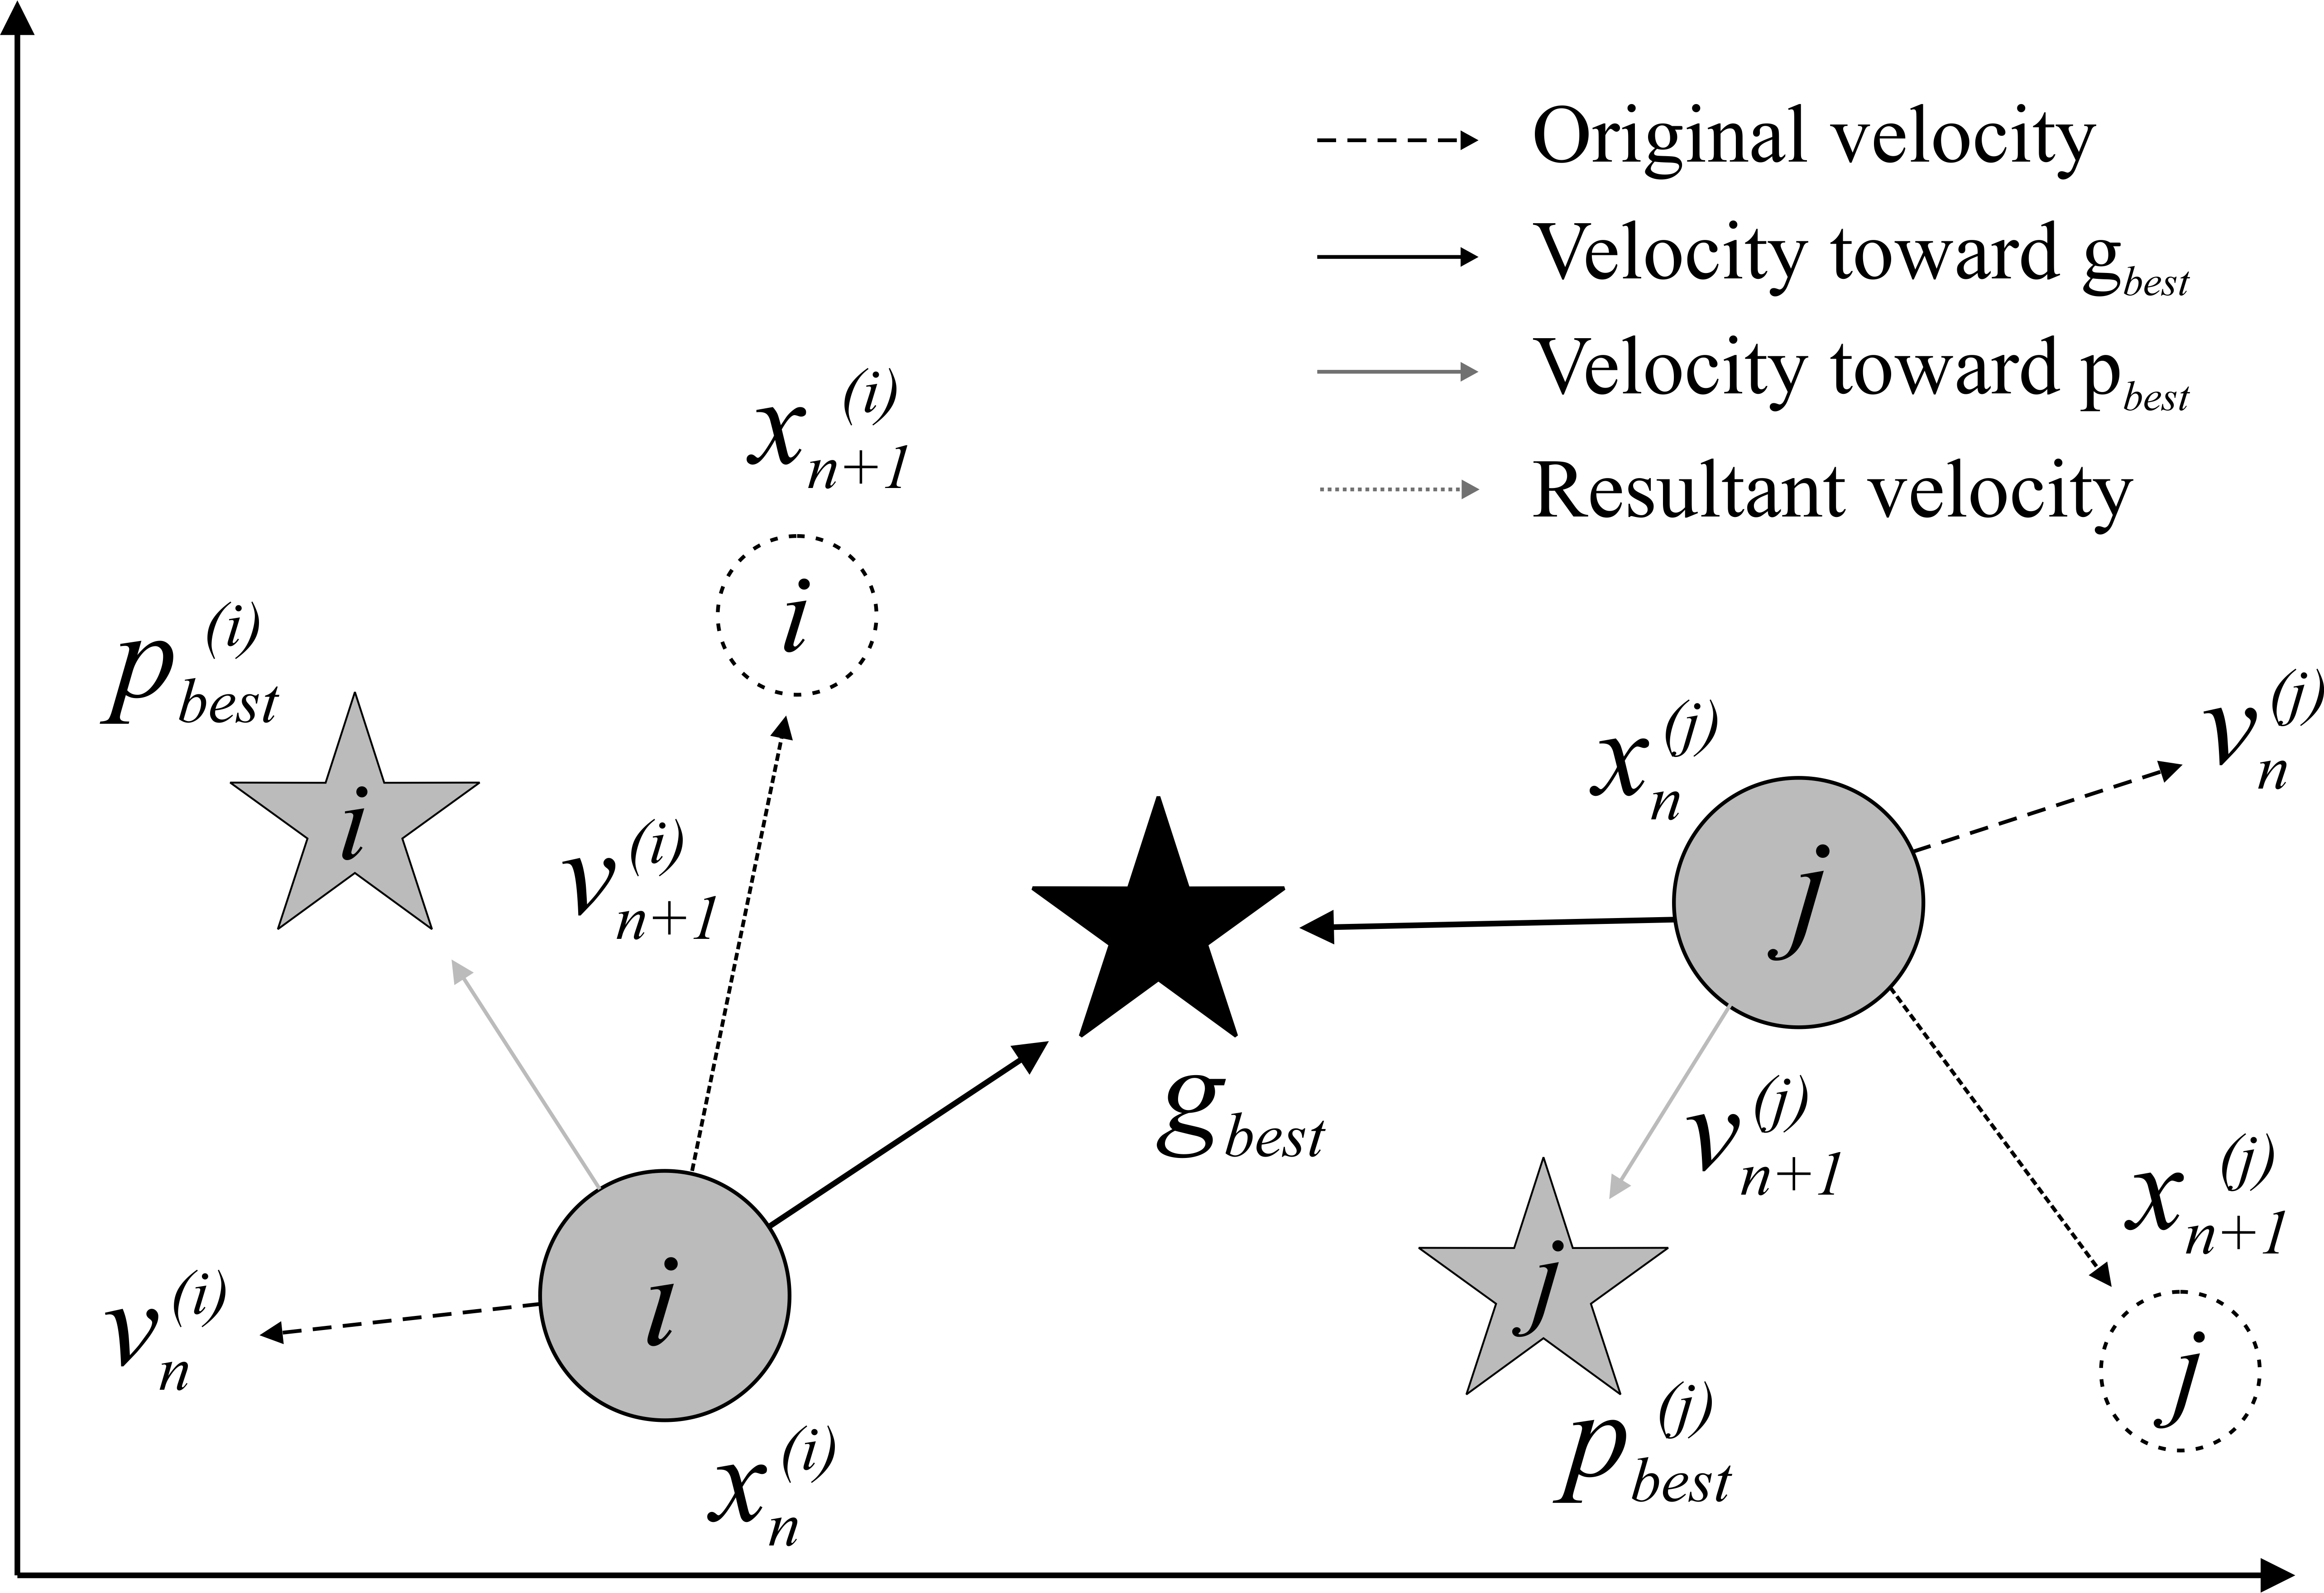
\includegraphics[width=\linewidth]{figs/pso_demo.png}
\caption{Mutations in PSO.}
\label{fig:pso}
\end{wrapfigure}


%%%%%%%%%%%%%%%%%%%%%%%%%%%%%%%%
\head{8. BROADER IMPACT AND EDUCATION:}
\paragraph{8.1. Benefits to Society at Large}
This proposal focuses on issues of
tremendous economic importance -- the creation of better quality software.
As a result, this work will increase America's ability for industrial and academic innovators to conduct
more scientific studies via computational means.  
 

\paragraph{8.2. Integration of Teaching and Research}
Much of the research in this project will also be integrated into a
classroom environment.  The PI teaches senior-level and graduate-level
SE, and software analytics   classes (and in those data mining
classes, all the case studies come from software engineering). All of
the technology developed in this proposal will become study
material for those subjects.  Replication studies are especially ripe
for classroom projects.  Also, through our publications and conference
work, we would publicize these tools as widely as possible with the
intent of supporting a broader community working with this approach.

\paragraph{8.3 Participation of Underrepresented
  Groups} The PI will continue their established tradition of
graduating research students for historically under-represented
groups.  PI Menzies' last two Ph.D. students were an African-American
women and a gentleman from an economically disadvantaged region
in central Pennsylvania.  Also, each summer, the PI's department runs an NSF-funded REU
 (research experience for undergraduates)
on the ``Science of Software''.
 At this
program, places are reserved for students from traditionally
under-represented areas (e.g. economically challenged regions of the
state of North Carolina) and/or students from universities
lacking advanced research  facilities.
Some of the simpler data mining concepts for this proposal would be suitable for lectures and REU projects.



%\input{f/under}
\paragraph{8.4. Dissemination of Knowledge}
 The PI has an extensive history of publishing at senior SE venues and so, it should be expected
that the results of this work will be widely visible.

Also, as mentioned above, the PI has a long history of publishing papers along with reproduction packages holding the data and the scripts required to
replicated the papers' results. All the our methods used here will be based around software tools in widespread   use (Github, Travis CI, etc).  We will release all our tools via open source licenses so our results can be readily applicable to researcher or developers using   Github, etc.
Although some of the data used in this study comes from private in-house projects,
the majority of our data comes open-source projects which we share with the community.

One issue here will be that it might be  too expensive
to let other groups download our  ingested data:
\bi
\item While we can certainly store our raw data on  S3,  Amazon   charges 4 cents per gigabyte download. Assuming our 5TB of data is downloaded 20 times a month for 3 years, that would cost \newline (\$0.05*1024*5*20)*36=\$184,320 $\approx$ 37\% of the grant (i.e. too much).
\item On the other hand, it is possible that our ingested data will occupy only a small fraction of the raw data-- in which case we can give free access
to our data to all
research groups.
\ei
Regardless of the above two points, we can certainly share all our scripts and bad smell detectors. These would allow other groups to replicated our results
after they conducted their own downloads.
 
 For more on this point, see our Data Management Plan.

 


\head{9. PRIOR RESULTS:}
This proposal is the next logical step in the PI's work on analytics.
{PI Menzies} has worked extensively in that arena.
In
\emph{``Automatic
Quality Assessment: Exploiting Knowledge of the Business Case''} (CCF-0810879, \$350,000, 08/08-06/11),
{PI Menzies} (with Bojan Cukic, WVU) built   generated many papers~\cite{jiang08a,me09n,me09i,me09b,me10d}
as well as one that is  was the third most-cited
paper in period 2009 to 2014 in the Journal of Empirical Software
Engineering.

In ``Better Comprehension of Software Engineering Data'' (CCF-1017330, \$500,000, 08/10-08/14).
{PI Menzies} (with Andrian Marcus, Wayne State),
explored various learning strategies (kernel estimation
methods, active learning tools, privatization methods) to
support defect and effort estimation. That work generated many papers~\cite{Bavota2010,Bavota2012a,Bavota2013,Bavota2012b,Haiduc2010a, Haiduc2013a, Haiduc2012a, Haiduc2013b, Marcus2010b, Ohlemacher2011b, Scanniello2013, Scanniello2011,me11m, peters12,Me13,me13a,peters12a}.
In terms \emph{broader impact}, that work graduated four masters and four Ph.D. students
and
spawned a small but active ``local learning'' research sub-community in SE (PI Menzies showed that
such ``local learners'' find better models
by first inferring local contexts, then building one model per context~\cite{Me13,me11m}).

  PI Menzies recently concluded
``Transfer Learning in Software Engineering'' (CCF-1302216, \$1,100,000, 08/13-07/18)
where {PI Menzies} (with Lucas Layman from Franhoufer Institute) 
building a toolkit to explore  methods for moving knowledge
learned from one software project to another.  That work  has generated
papers at TSE'18~\cite{krishna2018bellwethers}, ICSE'15~\cite{PetersML15}, ASE'15~\cite{krishna16}  and ESEM'13~\cite{he13} as well as the EMSE journal~\cite{Me17}, two IST journal papers~\cite{fu2016tuning,krishna2017learning},
one TSE paper~\cite{nam2017heterogeneous}.   A surprising and very useful outcome of that work
was the discovery of ``bellwethers'',  a simple transfer learner.

 PI Menzies has been working on  ``Scalable Holistic Autotuning for Software Analytics''
(CCF-1703487, \$898,349, 7/1/17-6/30/21) which is work with Co-PI Xipeng Shen
on using compiler technology to optimize very slow software analytics workflows. 
That work has several journal papers currently under review.

Also, since May'18 PI Menzies has worked on 
 EAGER: Empirical Software Engineering for Computational Science (CCF-1826574, \$124,628.00) looking at methods for applying empirical SE to computational science.
 That time has been spent interviewing domain experts and collecting data from
 Comp.Sci. projects.



% For the reader familiar with recent work~\cite{Siegmund17,DAngelo17,Fritz14} 
% discussing the how programming is informed by neuroscience  
%  (e.g. using EEG monitoring , eye tracking etc.), we make the following
% remark: this proposal takes more of a cognitive science approach, than a neuroscience approach.
% Neuroscience is very informative on how individuals process information in milliseconds
% to seconds; e.g. how a  programmer's eye flits around a block of code. Our task is
% different  since we are  concerned with how communities build/share/maintain their rules to control
% software project quality. Such building/sharing/maintaining takes days/weeks/months/years.
% Hence we are more concerned with model building (which is a cognitive issue) than how
% programmer's instantly react to new information (which is a neuroscience issue).
 
 
% For the reader familiar with Bayes networks and their application to software engineering~\cite{hearty2009predicting,okutan2014software,misirli2014bayesian,dejaeger2013toward},
% we note that such networks can be used to combine expert intuition (sketched out in the form of
% a directed graph combining influences in a software system) and a data mining
% method to incrementally update those networks as new information arrives. We do not use those here, due to some advice from Fenton et al.~\cite{hearty2009predicting} who have had much
% experience with conducting extended workshops with business users in order to capture their intuitions (about software quality)
% in a network structure. 
%  Fenton (personnel communication)  reports that such direct knowledge acquisition methods (where experts
% are asked about their expertise directly) can be very labour intensive. Specifically, it took 2 years to build one network 
% using input from 15 business users. Such direct acquisition methods do not scale so this research explores other approaches.

% Another technique that tries to combine human knowledge with AI methods is to use algorithms informed by crowd-sourced input (e.g.
% using tools like Mechanical Turk).
% For example, Heikinheimo and Ukkonen’s
% centroid median theorem~\cite{HeikinheimoU13} shows that if a
% crowd checks numerous examples for outliers,
% then the item least marked as an outlier is equal to the mean of a univariate normal distribution.  That
% is, crowds can be used as a human-based data miner to implement, for example, a crowd sourced K-means
% clusterer (as done by Heikinheimo and Ukkonen).  Our prior work with crowd-based reasoning~\cite{chen2017replicating} showed us that
% the wisdom of the crowd has to be carefully collected and curated-- an approach that may not scale to to the millions of
% developers using our cloud platform. Further, once the crowd is polled, there still needs to be some mechanism that handles conflicting
% opinions within the cloud (which we do with PSO). In summary, while crowd-sourcing is certainly a useful approach, it only addresses
% a small portion of our problem (and even in that small portion, there are scalability issues).

% Planning  has been a subject of much research in artificial intelligence. Here, planning usually refers to generating a sequence of actions that enables an \textit{agent} to achieve a specific \textit{goal}~\cite{norvig}. This can be achieved by classical search-based problem solving  approaches or logical planning agents. Some of the most common planning paradigms include: (a) classical planning~\cite{wooldridge95}; (b) probabilistic planning~\cite{altman99}; and (c) preference-based planning~\cite{baier09}. Existence of a model precludes the use of each of these planning approaches. This is a limitation of all these planning approaches since not every domain has a reliable model. In software engineering, the planning problem translates to proposing changes to software artifacts. Solving this has been undertaken via the use of some search-based software engineering techniques~\cite{Harman2009}. In some software engineering domains there is ready access to such models which can offer assessment of newly generated plans, e.g, automated program repair~\cite{Weimer2009, LeGoues2015}, software product line management~\cite{sayyad13, henard15}, etc. However, not all domains come with ready-to-use models. For example, consider software defect prediction. A model that includes {\em all} those potential issues would be very large and complex. In such domains, we seek alternate methods for planning that can be automatically updated with new data without comprehensive models. 

% Yet another related AI technique that combines human opinion and AI is active learning. In this approach, some classifier reflects
% over the space of examples seen so far to determine the next most useful example to evaluate~\cite{YuKM16}. In this way, active learning reduces
% the number of times an inference engine pesters a human expert for an opinion. While an interesting approach, it is not useful here for two reasons: (a) it is focused on classification (our task is planning); (2) In our domain we have no shortage of experts eager to point out our mistakes. So while we have conducted experiments with active learning elsewhere~\cite{YuKM16}, they is not relevant here.



%  \begin{wrapfigure}[11]{r}{3in}
\scriptsize
  
  
 \begin{tabular}{{l@{~~~~}l@{~~~~}|r@{~~~~}r@{}c@{~~~}r}}
\arrayrulecolor{lightgray}
\rowcolor{lightgray}\textbf{Rank} & \textbf{Treatment} & \textbf{Median} & \textbf{IQR~~~} & \\
  1 &         CrossTree &    56   &  21  & \quart{54}{25}{65}{1} \\
\hline  2 &        Alves &    32   &  17  & \quart{28}{20}{37}{1} \\
\hline  3 &     Shatnawi &    15   &  4.2 & \quart{15}{6}{18}{1} \\
\hline \end{tabular}

 
% \textbf{Poi}~~~~~~~~ \begin{tabular}{{l@{~~~~}l@{~~~~}|r@{~~~~}r@{~~}c@{}r}}
% \arrayrulecolor{lightgray}
% \rowcolor{lightgray}\textbf{Rank} & \textbf{Treatment} & \textbf{Median} & \textbf{IQR~~~} & \\
%         1 &         CrossTree &    20   &  16  & \quart{39}{40}{51}{2} \\
% \hline  2 &        Alves &    14   &  16  & \quart{21}{41}{37}{2} \\
%         3 &     Shatnawi &    8   &  1  & \quart{19}{5}{21}{2} \\
% \hline \end{tabular}\\
 
\caption{Somewhat quality
improvement seen in 30 random samples of the data.
measured in terms of $G=100\times(1- v/u)$ (defined in text).
Comparing the effectiveness of CrossTREEs's plans to other methods on two defect data sets.
Median, IQR are 50th   (75-25)th percentiles values.
{\em Larger} values
are {\em better}).
From~\cite{Kr16}.}\label{fig:xtree_results}
\end{wrapfigure}
% {\scriptsize \textbf{Lucene}~ \begin{tabular}{{l@{~~~~}l@{~~~~}|r@{~~~~}r@{~~}c@{}r}}
% \arrayrulecolor{lightgray}
% \rowcolor{lightgray}\textbf{Rank} & \textbf{Treatment} & \textbf{Median} & \textbf{IQR~~~} & \\
%         1 &         CrossTree &    16   &  6  & \quart{50}{29}{71}{4} \\
%         1 &     Shatnawi  &    15   &  2  & \quart{63}{10}{67}{4} \\
% \hline  3 &        Alves  &    9   &  4  & \quart{33}{19}{42}{4} \\
% \hline \end{tabular}}\\
% {\scriptsize \textbf{Ivy}~~~~~~~~ \begin{tabular}{{l@{~~~~}l@{~~~~}|r@{~~~~}r@{~~}c@{}r}}
% \arrayrulecolor{lightgray}
% \rowcolor{lightgray}\textbf{Rank} & \textbf{Treatment} & \textbf{Median} & \textbf{IQR~~~} & \\
%         1 &        Alves &    67   &  20  & \quart{58}{21}{71}{1} \\
% \hline  2 &         CrossTree &    52   &  22  & \quart{42}{24}{55}{1} \\
% \hline  4 &     Shatnawi &    20   &  7  & \quart{18}{8}{21}{1} \\
% \hline \end{tabular}}\\
% {\scriptsize  \textbf{Jedit}~~~~~ \begin{tabular}{{l@{~~~}l@{~~~~}|r@{~~~~}r@{~~}c@{}r}}
% \arrayrulecolor{lightgray}
% \rowcolor{lightgray}\textbf{Rank} & \textbf{Treatment} & \textbf{Median} & \textbf{IQR~~~} & \\
%   1 &        Alves &    36   &  7  & \quart{60}{10}{66}{1} \\
%   1 &        CrossTree &    36   &  0  & \quart{66}{0}{66}{2} \\
%   1 &     Shatnawi &    36   &  9  & \quart{53}{13}{66}{1} \\}
%  CrossTREE   is known to generate effective plans  for improving software quality in many   software engineering domains.
% With Krishna et al.~\cite{krishna2017learning,krishna16,Kr16}, we have  applied CrossTREE
%  plans  to data relating to (a)~predicting issue close time in Github;
% (b)~effort estimation; (c)~bad smell detection; and  (d)~defection prediction data. 
% In all those domains, Krishna et al.~\cite{krishna2017learning,krishna16,Kr16} showed
%  that CrossTREE plans are an effective tool for proposing effective changes to software projects.
%  For example, \fig{xtree_results} shows some CrossTREE results for defect prediction.
% In this study,
% CrossTREE's plans were compared against alternate
% plans generated by methods proposed by Alves, Erni, Hermans, Shatnawi et al.~\cite{Al10},~\cite{Er96},~\cite{He15}, and~\cite{Sh10}. These tools were used to assess CrossTREE since they are very  widely cited (as of August 2017, Google Scholar reported that the Alves, Erni, Hermans,and Shatnawi's papers have received  118, 116, 23, and  85 citations, respectively).
% All these methods raise an alert if some static code measure crosses some decision boundary;
% e.g. Erni et al. raises an alert if any static code measure is above  $\mu+\sigma$  for that static code measure's distribution. 

% To compare CrossTREE against these other tools, the following procedure was applied.
% First, the available project data was divided into separate {\em train, change} and {\em test} set.
% Second, Random Forests were applied to the {\em train} set to learn a verification oracle that can predict the bug-proneness of some section of code.
% Random Forests were used since Ghotra and Lessmann et al.~\cite{Gh15},~\cite{Le08} both strongly recommend Random Forest.
% Third,  CrossTREE and the other methods were applied to the {\em change} set to generate planners to plan for what to change. For CrossTREE, the planner was generated as per  \fig{tutorial}.
% For the other methods, the planners were obtained by adhereing to the thresholds at which these tools raised an alert.
% Fourth, we applied the changes recommended in step-3 to the {\em test} set.
% Fifth, using the verification oracle built in step-1, we determined how many bugs would be seen if the code was changed as per step~4.
%  \fig{xtree_results} shows the resulting performance measures in terms of
%   $G=100\times(1- v/u)$ where {\emu u,v} denote the probability of low
% quality before, after applying a plan. 
% Values near 0
% imply no improvement and {\em larger} values are {\em better}.
% The $G$ values seen using
% CrossTREE's plans are {\em larger},  hence {\em better} that other methods. 


% % \begin{wraptable}{r}{3in}
% % \small
% % \begin{tabular}{|p{.95\linewidth}|}\hline
% % {\em Question~1: ``Do bellwethers guarantee permanent conclusion stability?''} No- and we should not expect them to. The aim of bellwethers is to {\em slow}, but do not  {\em stop}, the pace of new ideas in software engineering. Sometimes, new ideas are essential. Software engineering is a very dynamic field with a high churn in techniques, platforms, developers and tasks. In such a dynamic environment it is important to change with the times. That said, changing {\em more} than necessary is not desirable- hence, bellwethers. 
% % \\\hline
% % {\em Question~2: `` How to detect when bellwethers need updating?''} 
% % Clearly, the conclusion stability offered by bellwethers only lasts as long as the bellwether remains useful. Hence, bellwether performance must always be monitored and, if that performance starts to dip, then seek a new bellwether. Later in this proposal, we will propose monitoring our models using {\em stream mining}.\\\hline
% % \end{tabular}
% % \caption{The Bellwether FAQ.}\label{tab:faq}
% % \end{wraptable}

% % \item
% % {\em What happens if a set of data has no useful bellwether?} In that case, there are numerous standard transfer learning methods that could be used to import lessons learned from other data~\cite{XXX}.  But we note that in our experiments, we have yet
% % to find another transfer learning method that is consistently better than the bellwether method.


% noindent{\bf2c. ``BELLTREE'': Planning Quality improvement.}
% Methods for addressing these challenges are addressed later in this paper.

% The next section of this proposal discusses our research questions and how we intend to address them. Before that, this section offers  notes on the BELLTREE planner~\cite{krishna19a,nair19a}. 
% The key point of BELLTREEs is that it creates
%   {\em very succinct} plans that mention only a few features. This brevity simplifies the  search for heterogeneous transforms (since there are  few features that need to be transformed).
%   Also, XXX readable. able to offer the trust needed by busines susers. XXXX also if used in a bellwether method offers th stability required so users have time to reflect on the models to gain insight.
%   XXXX
% \begin{figure}[!t]
%  \hrule
 
%  \begin{minipage}{.59\linewidth}
%  \vspace{1mm}
% \includegraphics[width=3.5in]{figs/XTREE_samp.eps}
% \end{minipage}
% \begin{minipage}{.40\linewidth}
% \small
% BELLTREE's plans 
% % from improving quality 
% are derived from decision trees or regression trees that predict for some software quality
% attribute. 
% In this example, the tree uses static code attributes to predict for number of bugs
% and the leaf values show the probability
% that a code module falling here will be buggy. 

% For example,  this decision tree is saying that
% the ``current branch'' has a `100\% chance of being buggy.
% BELLTREES's  {\em plan} is the {\em delta $\Delta$} between
% a test instance's current leaf and a nearby {\em desired} leaf with higher quality.
% \end{minipage}
% \hrule
% \caption{BELLTREES: generating plans from decision tree branches. From~\cite{Kr16}.}\label{fig:tutorial}
% \end{figure} 
% Formally, we distinguish {\em planning} from {\em prediction} as follows.
% {\em Predictors} in software analytics take the form \mbox{$out = f(in)$}
% where {\em in} contains many independent features (such as OO static code metrics) and {\em out} contains some measure of
% software quality such as how many defects are present. For software analytics, the function $f$ is learned via data mining (from static code attributes for instance).
% On the other hand, a quality {\em planner} generates a concrete set of actions that can be taken (as precautionary measures) to significantly reduce the likelihood of defects occurring in the future. More specifically,   consider a software artifact $Z$ (e.g. a code module).


% \newpage \noindent Planners
% proposes a plan $\Delta$ to adjust attribute $Z_j$ as follows:

% %{\scriptsize \begin{equation*}
% {\small \[\forall \delta_j \in \Delta :  Z_j =  
% \begin{cases}
%      Z_j + \delta_j& \text{if $Z_j$ is numeric}\bigstrut[t]\\
%     \delta_j              & \text{otherwise}
% \end{cases}\]}
% With a planner, to (say) simplify a large bug-prone method, our planners
% might suggest to a developer to reduce its size (i.e. refactor that
% code by, say, splitting it across two simpler functions). 
 
 


% XXXX need the charts here on how to plan.

%  \begin{wrapfigure}[11]{r}{3in}
\scriptsize
  
  
 \begin{tabular}{{l@{~~~~}l@{~~~~}|r@{~~~~}r@{}c@{~~~}r}}
\arrayrulecolor{lightgray}
\rowcolor{lightgray}\textbf{Rank} & \textbf{Treatment} & \textbf{Median} & \textbf{IQR~~~} & \\
  1 &         CrossTree &    56   &  21  & \quart{54}{25}{65}{1} \\
\hline  2 &        Alves &    32   &  17  & \quart{28}{20}{37}{1} \\
\hline  3 &     Shatnawi &    15   &  4.2 & \quart{15}{6}{18}{1} \\
\hline \end{tabular}

 
% \textbf{Poi}~~~~~~~~ \begin{tabular}{{l@{~~~~}l@{~~~~}|r@{~~~~}r@{~~}c@{}r}}
% \arrayrulecolor{lightgray}
% \rowcolor{lightgray}\textbf{Rank} & \textbf{Treatment} & \textbf{Median} & \textbf{IQR~~~} & \\
%         1 &         CrossTree &    20   &  16  & \quart{39}{40}{51}{2} \\
% \hline  2 &        Alves &    14   &  16  & \quart{21}{41}{37}{2} \\
%         3 &     Shatnawi &    8   &  1  & \quart{19}{5}{21}{2} \\
% \hline \end{tabular}\\
 
\caption{Somewhat quality
improvement seen in 30 random samples of the data.
measured in terms of $G=100\times(1- v/u)$ (defined in text).
Comparing the effectiveness of CrossTREEs's plans to other methods on two defect data sets.
Median, IQR are 50th   (75-25)th percentiles values.
{\em Larger} values
are {\em better}).
From~\cite{Kr16}.}\label{fig:xtree_results}
\end{wrapfigure}
% {\scriptsize \textbf{Lucene}~ \begin{tabular}{{l@{~~~~}l@{~~~~}|r@{~~~~}r@{~~}c@{}r}}
% \arrayrulecolor{lightgray}
% \rowcolor{lightgray}\textbf{Rank} & \textbf{Treatment} & \textbf{Median} & \textbf{IQR~~~} & \\
%         1 &         CrossTree &    16   &  6  & \quart{50}{29}{71}{4} \\
%         1 &     Shatnawi  &    15   &  2  & \quart{63}{10}{67}{4} \\
% \hline  3 &        Alves  &    9   &  4  & \quart{33}{19}{42}{4} \\
% \hline \end{tabular}}\\
% {\scriptsize \textbf{Ivy}~~~~~~~~ \begin{tabular}{{l@{~~~~}l@{~~~~}|r@{~~~~}r@{~~}c@{}r}}
% \arrayrulecolor{lightgray}
% \rowcolor{lightgray}\textbf{Rank} & \textbf{Treatment} & \textbf{Median} & \textbf{IQR~~~} & \\
%         1 &        Alves &    67   &  20  & \quart{58}{21}{71}{1} \\
% \hline  2 &         CrossTree &    52   &  22  & \quart{42}{24}{55}{1} \\
% \hline  4 &     Shatnawi &    20   &  7  & \quart{18}{8}{21}{1} \\
% \hline \end{tabular}}\\
% {\scriptsize  \textbf{Jedit}~~~~~ \begin{tabular}{{l@{~~~}l@{~~~~}|r@{~~~~}r@{~~}c@{}r}}
% \arrayrulecolor{lightgray}
% \rowcolor{lightgray}\textbf{Rank} & \textbf{Treatment} & \textbf{Median} & \textbf{IQR~~~} & \\
%   1 &        Alves &    36   &  7  & \quart{60}{10}{66}{1} \\
%   1 &        CrossTree &    36   &  0  & \quart{66}{0}{66}{2} \\
%   1 &     Shatnawi &    36   &  9  & \quart{53}{13}{66}{1} \\}
%  CrossTREE   is known to generate effective plans  for improving software quality in many   software engineering domains.
% With Krishna et al.~\cite{krishna2017learning,krishna16,Kr16}, we have  applied CrossTREE
%  plans  to data relating to (a)~predicting issue close time in Github;
% (b)~effort estimation; (c)~bad smell detection; and  (d)~defection prediction data. 
% In all those domains, Krishna et al.~\cite{krishna2017learning,krishna16,Kr16} showed
%  that CrossTREE plans are an effective tool for proposing effective changes to software projects.
%  For example, \fig{xtree_results} shows some CrossTREE results for defect prediction.
% In this study,
% CrossTREE's plans were compared against alternate
% plans generated by methods proposed by Alves, Erni, Hermans, Shatnawi et al.~\cite{Al10},~\cite{Er96},~\cite{He15}, and~\cite{Sh10}. These tools were used to assess CrossTREE since they are very  widely cited (as of August 2017, Google Scholar reported that the Alves, Erni, Hermans,and Shatnawi's papers have received  118, 116, 23, and  85 citations, respectively).
% All these methods raise an alert if some static code measure crosses some decision boundary;
% e.g. Erni et al. raises an alert if any static code measure is above  $\mu+\sigma$  for that static code measure's distribution. 

% To compare CrossTREE against these other tools, the following procedure was applied.
% First, the available project data was divided into separate {\em train, change} and {\em test} set.
% Second, Random Forests were applied to the {\em train} set to learn a verification oracle that can predict the bug-proneness of some section of code.
% Random Forests were used since Ghotra and Lessmann et al.~\cite{Gh15},~\cite{Le08} both strongly recommend Random Forest.
% Third,  CrossTREE and the other methods were applied to the {\em change} set to generate planners to plan for what to change. For CrossTREE, the planner was generated as per  \fig{tutorial}.
% For the other methods, the planners were obtained by adhereing to the thresholds at which these tools raised an alert.
% Fourth, we applied the changes recommended in step-3 to the {\em test} set.
% Fifth, using the verification oracle built in step-1, we determined how many bugs would be seen if the code was changed as per step~4.
%  \fig{xtree_results} shows the resulting performance measures in terms of
%   $G=100\times(1- v/u)$ where {\emu u,v} denote the probability of low
% quality before, after applying a plan. 
% Values near 0
% imply no improvement and {\em larger} values are {\em better}.
% The $G$ values seen using
% CrossTREE's plans are {\em larger},  hence {\em better} that other methods. 
  
  
  
% While the above results are promising, they clearly suffer from at least two major drawbacks. N2 and hyperparamter optimization. hwo to find the commuity. in the above, done manually. 

% The rest of this proposal proposed innovative methods for addreessing the above two drawbacks.

% % Further to the That said,   we would still recommend trying bellwethers before moving on to more complex methods. In his text on empirical software engineering, Cohen~\cite{cohen95} recommends benchmarking supposedly more sophisticated methods against simpler alternatives. Hence we  recommend that  bellwethers be applied first as a baseline method against which they other more complex methods
% % can be tested.  
% %\ee
% or classification,
% the BELLTREE algorithm looks for deltas in the model learned via belle



% \begin{wraptable}{r}{3in}
% \caption{Software analytics can be applied to many kinds of SE project data. }\label{tbl:types}
% \begin{tabular}{p{.95\linewidth}}\hline
%   \rowcolor{gray!10}
% \small
% \begin{itemize}[noitemsep,topsep=0pt,leftmargin=2mm]
% \item
% Unstructured  text resources; e.g. topic modeling for
% Stackoverflow~\cite{amrti18} or sentiment analysis on 
% programmer comments~\cite{msr18papercomparingsentimenttools}; \item
% Personnel and large-scale product data~\cite{rahulTemporalModelingMar18};
% \item
% Traces of complex run-time network behavior~\cite{shameli2014taxonomy};
% \item Large scale queries to the abstract
% syntax trees of softare projects~\cite{boareference}.
% \item
% Older-style 
% source-code metrics using, e.g., object-oriented -K metrics~\cite{weFSE17};
% \item Etc.
% \end{itemize}
% \vspace{2mm}
% \hline
% \end{tabular}
% \end{wraptable}
%  ~{\bf RQ1} is a pressing and important  current issue.
% In the very near future, 
% more engineers will apply  more  data miners to more  SE data.   There are many reasons for this.
% Firstly, the amount of data growing for automated software analytics is  increasing. For example, via Github, it is now possible to access code,  discussions, issue reports, etc on over 50 million projects.  Secondly, as seen in Table~\ref{tbl:types},
% the range of useful software analytics tools is
% increasing.
% Thirdly,
% the number of engineers skilled in these tools is ever increasing since most graduate (and even undergraduate) degrees include numerous classes on data mining.

% Our concern is the following scenario. Suppose that
% after all those
% engineers  run all that data miners on all that data,
% {\em they never reach the same conclusions}. This is not
% an ideal speculation  since the experience to date is that the models learned from SE data is not stable. 
% Even after a decade of  collecting project, 
% software analytics researchers report that {\em more} projects
% they sample, the {\em greater} the divergence in the learned
% models~\cite{ISTeditorial}.  Later in this proposal,
% we discuss the many causes of such variablity.

% Accordingly this project explores {\em scalable learning}
% using {\em stability operators} in order to test
% for the presence of {\em stable conclusions} in large
% corpora of SE data.  Since SE is such a diverse process,  we  guess
% that 
% the conclusions of  one model will not hold across all software projects.
% Hence we will seek  (a)~stable conclusions
% that hold across  a large numbers of similar projects;
% and (b)~mechanisms for discovering those groups of similar  groups. We call such mechanisms {\em context discovery tools}
% and these too will be explored in this work.


% \noindent{\bf Technical Innovations:} transfer. XXX scalability. planning. heterogenous . spectral clustering. stream mining. moea, fousing on stability.


% \noindent{\bf Data Availability:} To test this work, we will use multiple data sources.
% As mentioned above, we have access to all the
% Github data.
% Also,   in other NSF work we are exploring 500+ systems
% used by the  
% computational scientists for tasks such as finite mesh analysis
% and the modeling of sub-molecular quantum effects

% \noindent{\bf Research Management Principles:}

% XXX RELATED WORK
% some stuff on universality
% some stuff on universal methods (e.g. the unsupevised work) but-- only been shown to be somewhat useful and even there it has been shown by many there are many interesting purposed for which the unsupervised fail. more generally, the unsupervised failed on the grounds of change minimlaity


% \section{4. Methods}
% Exploit a trick in wolpert. Find two sets of betters

% One way to view this is a  clustering problem. Hw to make clustering
% easier? Have some reverse index. Here we propose best learner" as the indexer.

% Another way to view this is a transfer learning problem. once we run a few learners, we can find L2> L1, then look over the rest of the space where L2>L1 the apply the L3 > L2. 

% once indexed, dumpe the elarned models and try to use the old model  at the very elast, taht is a baseline against which a new learner can be compared. at the very most, the old will work well.


 
% \section{2. Why study stability?}
% Wcience is geranlity.

% Many learners 
% use stochastic sub-routines (e.g. neural nets,
% search-based evolutionary methods) and so their
% learned structures may change from run to run.
% Other learners are known to improve dramatically if their
% control parameters are adjusted (via hyperparater)
% This proposal is concerned with the stability of models
% learned from very large data SE data sets.
% Stability is an issue  

% But is stability an important issue? Can it be ignored and we still achieve success in software analytics? So far, the  evidence is that in many different domains, automated software analytics can deliver
% models that can predict, with sufficient veracity,
% quality aspects of a project~\cite{refs}. Note that
% the internal details of  those models may be  highly variable:
% \bi
% \item
% e.g. 
% due to its stochastic nature, a deep learner may generate
% a different internal network, each time it is run;
% \item
% e.g. Fig1 shows a very wide divergence in the  $\beta_i$ parameters returned by
% a learning generating  a linear model $y=\beta_0 + \sum_i\beta_ix_i$ across 20 different samples of
% 90\% of the training data.ZZZ
% \ei
% But if all this model variability
%  usually offer
%  reasonable predictions, who cares if their internal
% forms are wildly different? To answer that question,
% we need to reflect on the {\em audience} of that model. 
% If the audience will accept the model without question,
% then model stability could be considered optional.

% XXX with sreaming and bayesin parameter optimization, XXX validation envelope (optimizaion now only as apexepensive as validation)

% XXXXidnex data via the learners they respond to.  when such matches try, experiment with useing modes from other data sets


% % For such domains, where no user will ever debate the conclusions, there are many candidate data mining algorithm
% % (see \tabl{bad}).
% However,  if a model's audience is a community of human
% software engineers, then that community is less likely to
% believe in a model if the model is constantly changing.

% Offering  believable stable insights is an important consideration
% in software analytics. 
% Numerous researchers stress that the ability to read and
% trust a model's output is essential to  trusting that model~\cite{menzies2014occam,  lipton2016mythos, dam2018explainable}.
% Trust is important since,
% according to Kim et al.~\cite{Kim2016},
%  software analytics aim to
%         obtain actionable insights
%         from software artifacts that
%         help practitioners accomplish tasks 
%         related to software development, systems, 
%         and users.          
   
%     In fact, Tan et al.~\cite{tan2016defining}   
%     that
%         for software vendors, managers, developers and users, 
%         such comprehensible  insights  are the core deliverable of software analytics. 
%         Sawyer et al. comments that actionable insight is the key driver for businesses 
%         to invest in data analytics initiatives~\cite{sawyer2013bi}.  
        
      
      
% ------------





% Perhaps note. 
% So far, the exper

% We would also hope for conclusions that are stable across
% \bi
% \item Different subsets of the data;
% \item Different releases and different years of the same project;
% \item Different parameter tunings of the model.
% \ei

% XXXX        
%   On the other hand     flly to keep stable XXXX
% To the best of our knowledge, only one team has offered experimental  evidence that
% any ``universal'' model exists (for defect prediction)
% but their approach required an extensive application of subject matter experts to define the ``best''
% features~\cite{Zhang16aa}. 
% It is not clear where to find such subject matter experts for 10,000
% projects for  {\bf Task123456} listed
% in our overview.

% \head{2. BACKGROUND:} 

% After many years of software analytics, we seem to have more questions
% than answers. 
% \bi
% \item
% The good news is that, in many SE domains, it has been seen
% that data miners can extract models that offer useful levels of 
% prediction (e.g.~\cite{czer11, ostrand04, Menzies2007a, turhan11, koc11b, export:208800, theisen15}). 
% \item
% But the bad news is that those models are often different from
% project to project.

% \ei
% So where are the  validated, trusted, and actionable insights
% that developers can apply to their specific 
% systems in order to improve those systems? 
% Certainly, many attempts have been made to
% record supposedly general principles of softawre engineering;
% see for example,   Endres \& Rombach's book  ``Empirical observations, laws, and theories''~\cite{endres2003handbook};  Glass's
% ``Facts and Fallacies of Software Engineering''~\cite{glass2002facts};
% ACM's   Software Book of Knowledge\footnote{https://www.computer.org/web/swebok};
% and their 
% recommendations regarding SE curriculum\footnote{For
% ACM's advice on curriculum for
% undergrad/graduate SE degrees, see 
% SE2014/GSwE2009 at https://www.acm.org/education/curricula-recommendations.};
% as well as numerous IEEE standards for best practices
% in software\footnote{e.g.
% see ISO/IEC/IEEE 12207 Systems and software engineering-  a software life cycle process standard  https://en.wikipedia.org/wiki/ISO/IEC_12207}. See also
% the proceedings of the ICSE SEMAT workshop series on software engineering method and theory

% That said, none of the above rises to the level of validated, trusted, and actionable insights. One problem is that they list {\em too many methods}, not
% all of which apply to a particular project.

% Perhaps not.
% Recently, we reviewed the results of a decade of SE
% data mining in the PROMSE project. In that work, the  {\em more} projects
% we sampled, the {\em greater} the divergence in the learned
% models~\cite{ISTeditorial}. 

% A typical
% software analytics paper learns models for 5-10 projects\footnote{need survey of MSR'18 data sets}. 
% This is odd since,
% thanks to on-line repositories like Github, we can access data from
% thousands of projects

% very active
% One possibility is that, as yet, we have not generalized
% from enough projects to learn effective models. A typical
% software analytics paper learns models for 5-10 projects\footnote{need survey of MSR'18 data sets}. 
% This is odd since,
% thanks to on-line repositories like Github, we can access data from
% thousands of projects\footnote{ To be precise,
% as of June 2018, GitHub  hosts  57 million repositories. However,  the {\em sanity checks} described later in this proposal show that only around $10^4$ represent concerted  effort by teams of developers.}.

% The central question of this proposal is this
% \begin{quote}
% {\em If we learned models from 1000s of SE projects,
% would that generate stable conclusions?}
% \end{quote}
% That is, would more data {\em confuse} or {\em clarify}
% our knowledge about software engineering.

% We ask this question since the experience of the PROMISE repository  There is a simple explanation of this. SE is a very
% diverse set of activities conducted by (a)~developers with  a wide range of skills that are (b)~building software for an ever changing set of goals for (c)~different users, for  (d)~an ever changing set
% of software and hardware development and delivery
% platforms
% (mainframe to pc to mobile to cloud to edge computing;
% Android or MacOs or Blackberry or  Windows or MacOs or Linux or other; C or C++ or Perl or Haskell or Python or Ruby or Go or Rust
% or Scala or Elixr etc).

% Recent results now increase our optimism in learning
% general models for SE. Transfer learning. etc. XXX. Note that none
% of these method were applied to the PROMISE results
% reported above. YYY very good results for effects of these models. regualrties based on language models also tells us regualriies exist within language models.XXX

% We will test these methods, on 1,000 to 10,000 of projects
% for new kinds of unstructured  text mining problems
% (reasoning about Stackoverflow questions or automatic
% assistance for source code ); software programmer sentiment;
% process and personnel issues (who should be involved 
% when code is committed; how to micro-adjust programmer resoruces on a month-to-month basis) ; as well as old-style software
% analytics problems
% source-code metrics (using, e.g. C-K metrics).

% Our test data will come from Github XXX IBM, and computational Physics.

% This lack of validated, actionable insights
% about SE is most strange.
% The past 50 years have seem remarkably progress in this field. 
% \bi
% \item
% Even for problems as complex as operating systems, 
% it is now possible for someone to sit
% on the floor of their mother's flat in Norway, and write software that 100s of millions of people around the world
% can download, execute, update and (if they are programmers),
% maintain, refactor, extend mash up with 1000s of other software tools~\cite{Torvalds01}. 
% \item
% Also, with minimal effort, it is now possible to use
% tools like Github to access
% data on tens of thousands of software projects including
% all source code, bug histories, and developer discussions.
% \item
% Further, given the current state
% of the art in software analytics, we now have tools
% that could, potentially,
% work through all that data looking for interesting
% conclusions. Not only can those tools handle traditional static code metrics but also
% process and personnel metrics (including time to close issues, who works on what parts of the code);
% complex unstructured textual entities (e.g. Stackoverflow or  
% text miners looking for  patterns in source
% code that predict for vulnerabities). 
% \item
% Lastly, even qualitative analysis is now scalable and,
% thanks to tools like Mechanical Turk, it is possible
% to explore the opinion space of a large number of skilled
% SE professionals\footnote{Note that while many members of the crowd worker population study is not qualified to comment on complex SE matters, repeated studies some that posting selection criteria, then carefully  screening the workers (e.g. using ``gold questions'' that ask about SE problems with known answers) it is still possible to find hundreds of crowd workers (within a population of a 1000 or more) that can offer detailed qualitative and quantitative  insights on SE problems. }.
% \ei

% %XXX need something about broad range
% % of problems: simple code attributes, complex text mining (stack overflow, text mining for security flaws); qualitative issues (scalable MT-- n

% Yet for all that, general principles of SE still allude us.
% Certain heroic attempts have been made to articulate
% general  principles of SE. .  To justify that last sentence, we cite two studies. Firstly, PremXXX
% Secondly, consider the experience of  PI Menzies, hired
% by NASA to review and improve their software verification
% and validation (V\&V) practices. There are many methods
% proposed for software V\&V in numerous high profile documents such as:
% \bi
% \item
% Wallace and Fujii's list of  20 essential and 36 optional tasks for software V&V.
% \item
% Table 2 of the IEEE-1012 standard for software V&V offers a list of 52 minimal tasks for IV&V. Each task is selected by a combination of development phase and estimated severity in project errors [2].
% \item Internal documents at NASA that list dozens of V\&V tasks.
% \ei
% But the literature, there are very few attempts to assess the relative cost-effectiveness of this broad range of V\&V techniques empirically. 
% \bi
% \item
% Several researchers offer detailed taxonomies of standard NASA faults [15,16], but do not address what tasks are most cost-effective at finding the faults. For example, Lutz reports studies on the most frequent kind of faults seen in deep-space NASA missions but does not fully address the issue of what V&V and IV&V tasks are best at removing faults [17].
% \item
% In a limited number of publications, some attempt is made to generalize over multiple projects, multiple methods, or projects extending over many years. For our purposes, these studies are incomplete. 
% \bi
% \item
% Some of this research bases its conclusions on just a few projects [5, 22, 23, 25].
% \item
% Others use a Delphi-style analysis were the authority of
% the conclusions rests on the authority of the author [6, 20, 21].
% \item
% Alternatively, they may base their conclusions on extensive data collection but, for confidentiality reasons, cannot make that data available for public scrutiny [26–28].
% \ei
% \item
% Just to say the obvious:
% it is hard to make critical audit conclusions based on a Delphi-style analysis or inaccessible data. 
% \ei
% \ei
% XXX saty this more carefully regarding data.
% In general, only a minority of SE researchers can publish the data used to make their conclusions (for example, [22–24,29,30]).
% Also, several of the these papers [27,28] only offer general advice about how to avoid problems in software development. The subjective nature of this advice makes it difficult to consistently deploy them over a national software development program. Only a few [23, 24, 29, 30] offer public- domain versions of their data and models.
% Note that, even in combination, the above publications cover a small fraction of the V\&V tasks listed in the literature.

% We propose a very specific test to search for generality in SE.
% {\em Stream miners}

% Seek more tha standard steam miners. reuse prior insigts. to as our stream miner excute, they query the results of other minres to check if their insights apply to us.



% Figure 3 offers 40 predeployment IV&V tasks

% optimism. sentiment. analysis of large scale unstructured text mining. process and personnel results , levering crowd (test analytics with crowd workers, scalable qualitative analysis with MT, automatic hyperparameter optimizers, transfer learning bellwethers.

% the last one is particularly relevant 

% {\em We have many doings, }but 
% % In 2013-2014, eleven million programmers \cite{abel14} and half a trillion dollars \cite{gartner14} were spent on information technology. Such a large and growing effort should be managed and optimized via well-researched conclusions. To assist in achieving this, there has been a growing recognition within the software engineering research community of the importance of systematic knowledge collection~\cite{paivarinta15},~\cite{sjoberg08},~\cite{stol2015theory}. Knowledge-building needs to be an iterative process, in which results from practice are used to refine knowledge, then that knowledge is  used to inform future observation and data collection \cite{paivarinta15},~\cite{stol2015theory}. It is no coincidence that it is standard practice in other fields, such as medicine, to continually revisit old conclusions in the light of new theories \cite{prasad13}.
% Software analytics distills large amounts of low-value data
% into small chunks of very high-value data. For example, after examining many software projects,
% it might be concluded that certain coding styles are more bug prone and, hence, should
% be depreciated.
% A challenging problem with     analytics is the pace of change
% in   software. Numerous results~\cite{Pa11,Jo09,De16,Me17} report   many prior beliefs
% about software engineering (SE) must now be revised due to the ever-changing nature of the tools,
% techniques, and practices.
% The hypothesis to be tested in this work is that we can create and maintain
%  better  up-to-date quality policies for software projects using  {\bf human-augmented data miners}. Participants at a recent
%  Dagstuhl meeting on software analytics~\cite{gall_et_al14}  agreed that human insight can, sometimes, add much value to an automatically 
%  learned models. For example,  Shull et al.~\cite{shull02} and Kocaguneli et al.~\cite{kocaguneli2013distributed} both report cases where human insight was critical to avoiding ridiculous errors in software analytics. Further, those insights were central to the creation of the final models (generated
%  as part of that work).

% But how to collect those insights in a manner that scales to include a very large number of projects?  Consider, for example, the cloud
% programming IDE developed 
% by our industrial partners here at the Raleigh Research Triangle, North Carolina. 
% This platform is an integrated DevOps tool that  build, run, deploy, and  manage  applications written in   Java, Node.js,  Go, PHP,  Swift,  Python,  Ruby  Sinatra,  Ruby  on Rails (and could  easily extended to support other languages  such  as  Scala).   At  the  time of this writing, this platform is used regularly by 1.6 million developers working on   1600 live projects on a variety of software analytics dashboards\footnote{There are  538 proprietary projects, plus over 1100 repositories marked as ``most trending'' at Github.}.  This cloud platform collects the {\em internal attributes} of \tab{metrics} which means, in turn,
% that our analytics tools can  find answers about the {\em internal quality attributes}
% shown in that table.
% The  dashboards of this IDE generate thousands of conclusions
% per day about all these projects  (later in this proposal, we give specific examples of those conclusions).

%  In theory, given all the developers   reflecting on all those conclusions,  it should be possible to obtain useful feedback from
%  a very large number of projects. 
%  To test if this is so,  we propose  an innovative  method that debates  different ideas about software quality. {\em Particle swarm optimization} (PSO)~\cite{banks2008review,banks2007review}  is used to implement an arena in which novel extensions to old ideas must
% compete to demonstrate their value (ideas without merit are ignored).  
% This approach  will be tested on    tasks
% such as (a)~predicting the time required to close issues; 
% (b)~predicting  how many developers should be assigned to a software task;
% (c)~predictors for the locations of bug in software;
% (d)~ planners for recommending methods to change all the above (which would be used if managers do not like the predicted values).
% These tasks are all ones that  PI Menzies has previously explored, using automatic data miners~\cite{Me13,krishna16,Kr16,rees2017better,Lu12,agrawal17,Me07,Me17}. Here, we extend that
%   work by asking:
 
%  \begin{center}
% {\em Are human-augmented data miners      
%  ``better'' for  software  analytics? }
% \end{center}
%  (i.e.,  ``better'' than  state of the art quality predictors or planners in the SE literature.)

 



 
% One significant feature of this work is its
% {\bf immediate industrial applicability}. We assert our research has such applicability  for two reasons.
% {\em Firstly},
% our methods
% will be based around software tools in widespread industrial use (Jira, Github, Travis CI, etc).  We will release all our tools via open source licenses so our
% results can be  readily applicable to the many research or development teams using Jira, Github, etc.


% {\em Secondly}, we will produce not only predictors but also {\em planners}
% for how to change software projects in order to improve quality with  that
%  project.
%  Why are such planners important? At a recent ASE'15 workshop on 
% ``Actionable Analytics''~\cite{Krishna15a}, industrial practitioners were very
% clear in their protest against complex software analytics that offer no insight on what to do in order to improve their projects.
% Much of the current work in software analytics, they said,  is on 
% {\em prediction} of ``what is'' rather than {\em planning}  of ``what to do''.
%  Accordingly, this proposal focuses particularly on the issue of generating plans describing what to do.
%   For a formal description on the difference between  planners and predictors,  see  \tab{planprd}.



% % Please add the following required packages to your document preamble:
% \usepackage{multirow}
\begin{table}[!t]
\scriptsize
\centering
\resizebox{.9\linewidth}{!}{
\begin{tabular}{l|ll}
\hline
\textbf{ENTITIES} & \multicolumn{2}{c}{\textbf{ATTRIBUTES}} \\  
\textit{\textbf{Products}} & \multicolumn{1}{c}{\textit{\textbf{Internal}}} & \multicolumn{1}{c}{\textit{\textbf{External}}} \\ \hline
\multirow{2}{*}{Specifications} & \multirow{2}{*}{\begin{tabular}[c]{@{}l@{}}size, reuse, modularity, redundancy, \\ functionality, syntactic correctness, \dots\end{tabular}} & \multirow{2}{*}{comprehensibility, maintainability, \dots} \\
 &  &  \\
\multirow{2}{*}{Designs} & \multirow{2}{*}{\begin{tabular}[c]{@{}l@{}}size, reuse, modularity, coupling, \\ cohesiveness, inheritance, functionality, \dots\end{tabular}} & \multirow{2}{*}{quality, complexity, maintainability, \dots} \\
 &  &  \\
\multirow{2}{*}{Code} & \multirow{2}{*}{\begin{tabular}[c]{@{}l@{}}CK metrics, McCabe metrics, Halstead metrics,  \\ functionality, algorithmic complexity,,control-flow structuredness, \dots\end{tabular}} & \multirow{2}{*}{\begin{tabular}[c]{@{}l@{}}reliability, usability, maintainability, \\ reusability\end{tabular}} \\
 &  &  \\
Test Data & size, coverage level, \dots & quality, reusability, \dots \\
\dots & \dots & \dots \\  
\textit{\textbf{Processes}} &  &  \\ \hline
\multirow{2}{*}{\begin{tabular}[c]{@{}l@{}}Construction\\ specification\end{tabular}} & \multirow{2}{*}{\begin{tabular}[c]{@{}l@{}}time, effort, \#requirement changes, \\ \dots\end{tabular}} & \multirow{2}{*}{quality, cost, stability, \dots} \\
 &  &  \\
\multirow{2}{*}{Detailed design} & \multirow{2}{*}{\begin{tabular}[c]{@{}l@{}}time, effort, number of specification faults\\ found, \dots\end{tabular}} & \multirow{2}{*}{cost, cost-effectiveness, \dots} \\


 &  &  \\
Testing & time, effort, number of coding faults found, \dots & cost, cost-effectiveness, stability, \dots \\
Maintenance & \#bug reports, \#maintenance requests, \#enhancement requests,\ldots & extensibleness\dots\\
            & \#issues open, \#issues closes, \#issue close time  \dots &   maintainability \dots \\
\dots & \dots & \dots \\  
\textit{\textbf{Resources}} &  &  \\ \hline
%Personnel & age, price, \dots & productivity, experience, intelligence, \dots \\
Teams & size, communication level, structuredness, \dots & productivity, quality, \dots \\
Organizations & size, pace of personnel change %ISO Certification, CMM level 
& Maturity, profitability, \dots \\
Software &   size, \dots & usability, reliability, \dots \\
%Hardware & price, speed, memory size, \dots & reliability, \dots \\
%Office & size, temperature, light, \dots & comfort, quality, \dots \\
\dots & \dots & \dots \\ 
\end{tabular}}
\caption{Some of the attributes we can access via mining of Github repositories and their associated tool chains.
Following  Fenton's~\cite{Fe14} guidance,  attributes are divided into product, process, and resource. Also, {\em internal}
metrics can be measured directly and {\em external} ones
represent the indirect external manifestations of the internal ones.  }
\label{tab:metrics}
\end{table}



% \head{2. MOTIVATION:  Why  New Tools?} 

% ~\\
 
% Before beginning, we digress to ask a basic question:
% why do we need new tools to discover insights about software projects? In this age of big data and  hyper-internet connectivity, is it not enough to just:
% \bi
% \item
% Run a few data miners?
% \item
% Or just ask someone; e.g. post a query to the on-line programmer forum  stackoverflow.com? 
% \ei
% Clearly, sometimes, there is  benefit in  knowledge found
% via automatic methods~\cite{Zimmermann2004}  or social qualitative methods~\cite{seaman1999qualitative}.
% However, neither approach is    foolproof. 
% Basili and Shull~\cite{shull02} warn that any automatic analysis of project data cannot access  tacit contextual
% knowledge known to humans, but not represented in any data set.
 
% \begin{figure}[t!]
    \centering
    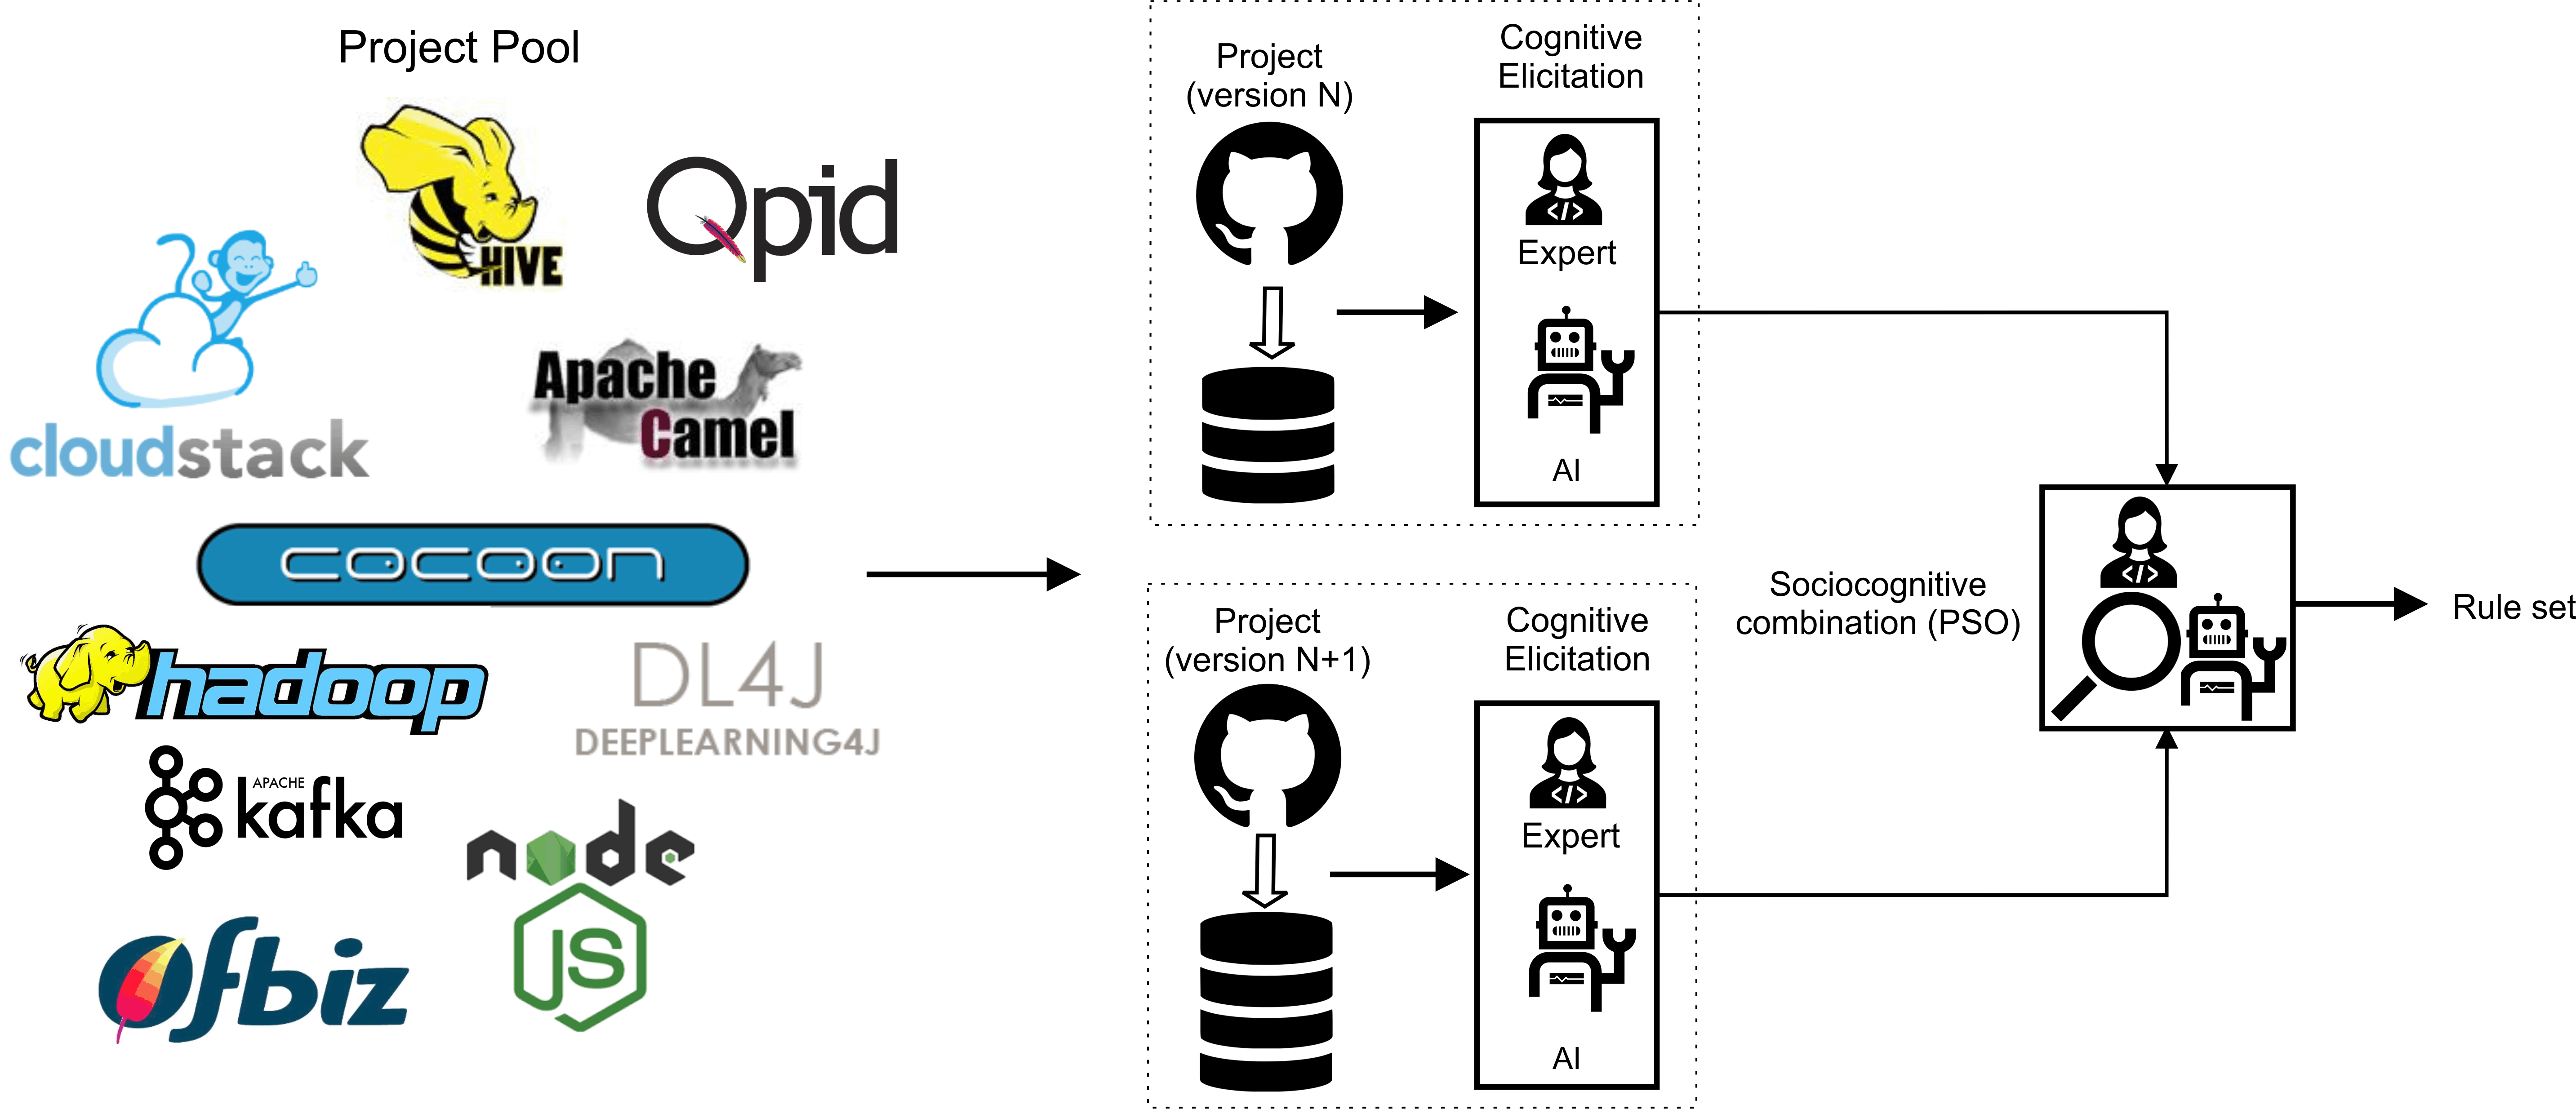
\includegraphics[width=\linewidth]{figs/flow.png}
    \caption{Flowchart of the proposed approach. Humans and AIs comment on data 
    from many projects. This knowledge enters an arena where competing ideas fight it out
    to conclude which are most useful. In this proposal, that arena will be implemented by particle swarm optimization.}
    \label{fig:flow}
\end{figure}

% As to eschewing data miners and just using supposed   expert opinion of
% developers, that  too  is  problematic.
%  Passos et al.~\cite{Pa11} warns that software developers often inappropriately assume whatever worked/failed on their first few projects will also work/fail on all their future projects. They comment  that ``past experiences were taken into account without much consideration for their context''~\cite{Pa11}. 
% Other  results by J\o rgensen \& Gruschke~\cite{Jo09} endorse the pessimism of Passos et al. In an empirical study of expert effort estimation, they report that the experts rarely use knowledge patterns from past projects to improve their future reasoning.  
% Yet other results have found numerous examples where developers hang on to old ideas, despite evidence to the contrary.
% Krishna et al.~\cite{Me17,Kr16}    have conducted   surveys of developers that
%   reveal widespread misconceptions and inconsistencies
% about the impact of delaying issue resolution in software systems;
% and the value (or otherwise) of fixing different kinds of code bad smells.
% In a more extensive study of programmers, Devanbu et al.~\cite{De16} surveyed 564 Microsoft software developers from around the world. They found that ``(a) programmers do indeed have very strong beliefs on certain topics; but (b) those beliefs can vary across the personnel within one project, and these usually do not necessarily correspond with actual evidence in that project.'' 

% So, what to do? Merely using data miners is not enough since they miss contextual knowledge. And merely
% asking developers can lead to misleading results. Perhaps a better way would be to combine human and artificial intelligence.

% % \head{3. OVERVIEW OF OUR APPROACH: Knowledge Elicitation and Combination} 


% % In the following, we propose a novel
% % {\em cognitive} approach that  combines {\em both}   human and artificial intelligence. Our hypothesis, to be tested in this research, is that better analytics 
% % arise  from {\em combining}
% %   (a)~an ability to reason over gigabytes of data
% %  with (b)~data mining with human contextual knowledge. Our approach is in two parts: 
% % \bi
% % \item A {\em cognitive elicitation method} that extracts developer insights 
% % about software. This elicitation method may be designed using data mining or by interacting with domain experts. 
% % \item A {\em socio-cognitive combination method}  that  combines multiple opinions into one coherent whole using  PSO~\cite{Eb95,banks2008review,banks2007review}. Here,  cognition 
% %  emerges from the convergence of the beliefs of many individuals. Note that PSO makes no
% %  assumption that any piece of knowledge is correct. Rather, it is an arena 
% %  where ideas must  compete to demonstrate their value.
% % \ei
% % For readers familiar with the AI literature, we note that alternate methods for combining human and artificial intelligence include Bayesian methods, 
% % crowdsourcing methods, and 
% % methods inspired by neuroscience. Those methods are not used here for reasons discussed in our {\em Related Work} section.

% % % TEXT HERE EXPLAIN FIGURE
% % The flow chart of the proposed scheme is shown in~\fig{flow}. For every project in the project pool, we mine the repositories and gather the necessary information. Next, we elicit cognitive insights from experts. For reasons discussed in \S2, we also seek to gather insights from tools like CrossTREE following which we combine these rules using a socio-cognitive approach (with PSO).  This approach overcomes a significant drawback with the  CrossTREE system:  CrossTREE has no knowledge on the {\em usability} of its recommendations. Hence, it is prone to produce recommendations that developers can not, or will not, want to change. Our plan is to elicit
% % feedback from developers to learn which recommendations are feasible (and which aren't).

% % \fig{venn} visualizes the space of used and ignored recommendations within a software project.
% % Here \circled{A} shows  all   artifacts that exist in a project and \circled{B} represents the artifacts that can be changed by the developers
% % of that project. 
% % Of that set, there is only a subset \circled{C} that developers are actually willing to change.
% %  \circled{D} is  a subset of the artifacts  that have been changed historically; and
% % \circled{E} represents the artifacts that CrossTREE recommends fixing. Note that the entire space of possibilities in \circled{A}~--~\circled{E} is not known, nor should we expect to know them. What we do get as the project evolves are a set of points that lie in these sets, i.e., if we watch the projects over time, then the pattern of \fig{venn} should appear. 

% % \begin{wrapfigure}[10]{l}{0.6\linewidth}
\footnotesize
\centering
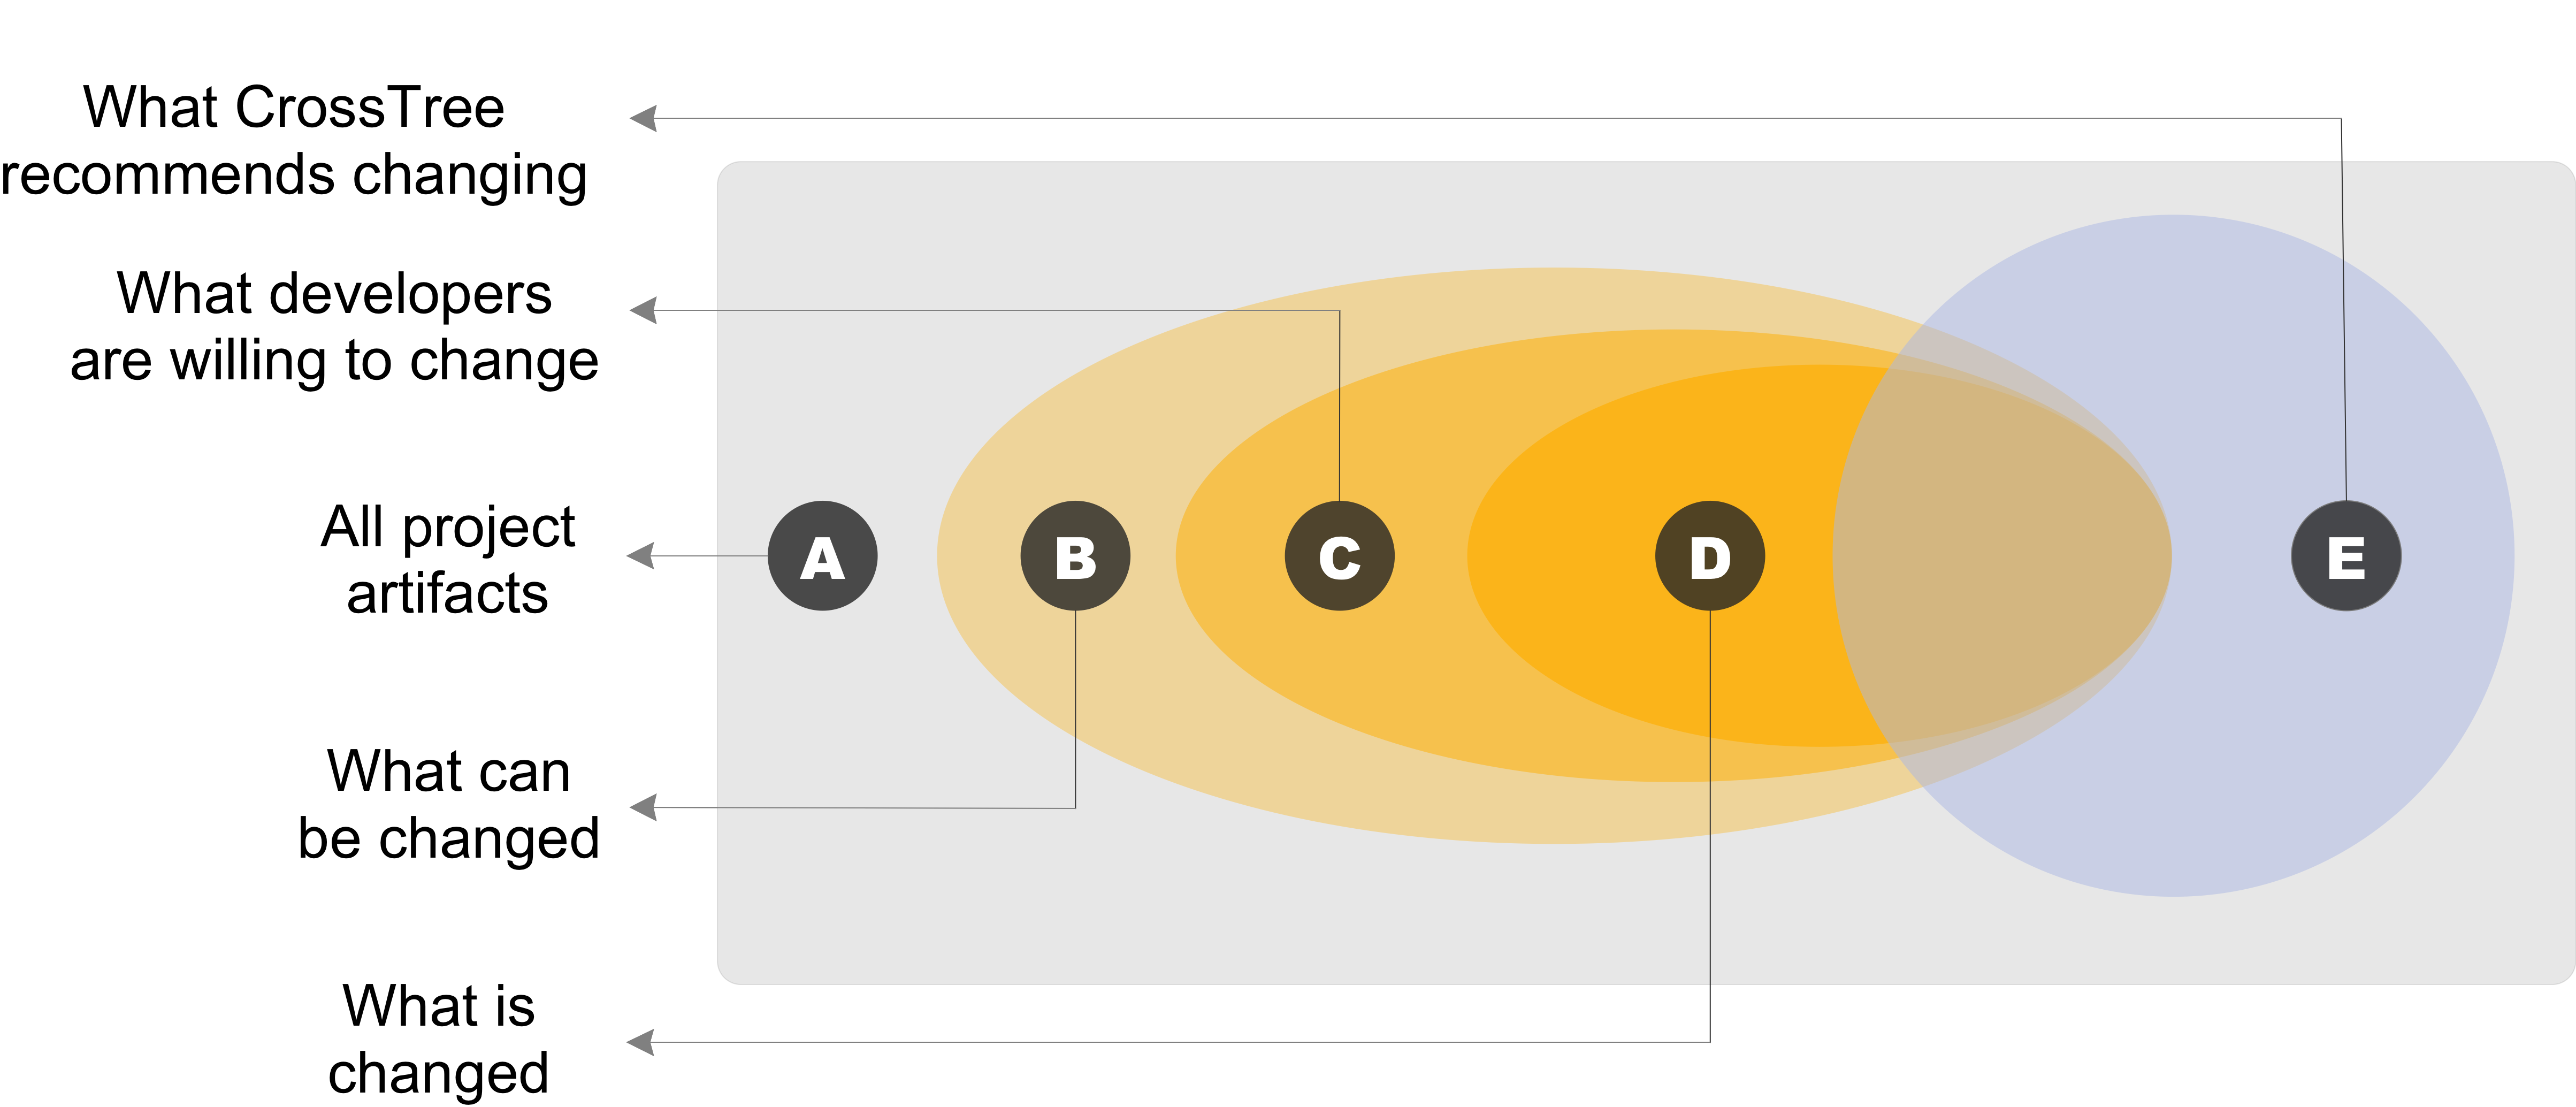
\includegraphics[width=\linewidth]{figs/venn.png}
\caption{Set of possible changes to address project artifacts.}
\label{fig:venn}
\end{wrapfigure} 

% % Using the sample point in the sets, we would say that developers have the following opinions about CrossTREE's recommendations:
% % \bi
% % \item {\em E=Endorsed} = $\circled{D} \cap \circled{E}$; i.e. the    recommendations   developers will actually use; 
% % \item {\em I=Irrelevant} =  $\circled{E} - \circled{B}$; i.e.  the recommendations  never used (and CrossTREE should avoid these);
% % \item {\em O=Other} = $\circled{D}- \circled{E}$; i.e. the  changes that developers made but which CrossTREE did not recommend.
% % \ei

% % The aim of this project is to explore the space of artifacts in~\fig{venn} so that the recommendations for improving software quality satisfies the following four goal multi-objective problem:
% % \bi
% % \item[1.]  {\em Maximize} $E$: the number of   {\em endorsed} recommendations;
% % \item[2,3.]  {\em Minimize} $I,O$: the  number of {\em irrelevant} and {\em other} recommendations;
% % \item[4.]  Maximize the  effectiveness of the recommendation as measured by the   $G$ equation of  \fig{xtree_results}.
% % \ei
% % \noindent We hypothesize that a socio-cognitive multi-objective evolutionary algorithm such as particle swarm optimization would be an ideal candidate for this purpose.

% % As a motivating example, for some project ``$X$'' assume that we have the internal attributes: $commit\_id$, $author$, $total\_loc$, $coupling\_between\_objects$, and $cyclomatic\_complexity$. Here, we have:
% % \bi
% % \item $\{\mathit{commit\_id,~author,~total\_loc,~coupling\_between\_objects,~cyclomatic\_complexity}\}\in \circled{A}$. The set of all artifacts, measured by a set
% % of attributes. Note that not all of these are changeable  so any recommendation to change (e.g.) {\em author} would be inappropriate.
% % Of these, 
% % \item $\{\mathit{total\_loc,~coupling\_between\_objects,~cyclomatic\_complexity}\}\in \circled{B}$. The set of all artifacts that can be changed.
% % \item $\{\mathit{coupling\_between\_objects,~cyclomatic\_complexity}\}\in \circled{C}$. The set of all artifacts that the developers are willing to change.
% % \item $\{\mathit{coupling\_between\_objects,~cyclomatic\_complexity}\}\in \circled{D}$. The set of artifacts that are changed.
% % \item And finally, $\{\mathit{commit\_id,~total\_loc,~cyclomatic\_complexity}\}\in \circled{E}$. The set of all artifacts that CrossTREE recommends changing.
% % \ei

% % \noindent From this, we can derive the following sets:
% % \bi
% % \item  {\em E=Endorsed} = $\circled{D} \cap \circled{E}$; i.e. $\{cyclomatic\_complexity\}\in E$
% % \item {\em I=Irrelevant} =  $\circled{E} - \circled{B}$; i.e.  $\{commit\_id\}\in I$
% % \item {\em O=Other} = $\circled{D}- \circled{E}$; i.e. $\{coupling\_between\_objects\}\in O$
% % \ei

% % \noindent The rules above would in fact be more concrete, e.g. {\em reduce cyclomatic complexity $<15$}. The developers reading these rules 
% % would keep track of the complexity of the modules they are developing, and split them into smaller modules whenever the cyclomatic complexity of the module exceeds 15. 

% % The above is an example of one set of insights. For real world projects, we have several thousand such rules which are constantly generated with new project data\footnote{For a real world example of this, see~\fig{bluemix} on page \pageref{fig:bluemix}}. In those cases, we would deploy a PSO with the objectives of: (1) maximizing $E$, (2-3) minimizing $I, O$, and (4) maximizing the effectiveness. The outcome of the PSO would represent the best subset of rules to be applied to a specific case.

% % \head{4. DETAILS}
% % This section motivates  our {\em elicitation} and {\em combination} methods
% % based on CrossTREE and PSO. These tools are developed using principles of cognitive
% % psychology,  described below. To summarize, we cannot just ask a large cloud of developers to state their knowledge. Rather, for reasons described below,
% % we will have to query it out of them. In the following, our ``trick'' will learn the useful sections of \fig{venn}.

% % \noindent
% % {\bf 4a On the Nature of Human Expertise: }
% % Recall from {\bf \S{2}}, the results of  Passos, J\o rgensen \& Gruschke, Krishna, 
% % Devanbu et al.~\cite{Pa11,Jo09,De16,Me17,Kr16}: human software developers have significant trouble explaining
% % their expertise.  
% % This is actually
% % a  known effect; specifically, even 
% % when humans are quite expert at some task, they can be   inept in explaining how they performed that task~\cite{Fi80,menzies1987micro,menzies94,Compton1990}.  This effect was first seen in the 1970s when researchers struggled to capture  human knowledge in ``expert systems''.
% % Those researchers found that experts were usually very slow at explaining their expertise;  and when they did, they would say contradictory or incorrect statements~\cite{Fi80}.  

% % Cognitive psychology~\cite{La81} offers an explanation for this puzzling behaviour of human expertise-- such expertise is stored in a large library of patterns that has been ``compiled'' in such a way as to support fast access, but not
% % easy browsing of the underlying knowledge. 
% % Larkin et al.~\cite{La81} characterize human expertise in terms of two memory structures:
% % \bi
% %     \item A very small short term memory, or STM, used as a temporary scratch pad for current observation. The short term  memory may be so small that it can hold only 7,  or even 4, items \cite{Mi56}, \cite{Co01}. Recently,  Ma et al.~\cite{Ma14} used evidence from neuroscience and functional MRIs  to  argue  that STM capacity might be better measured using other factors than ``number of items''. But even they conceded that ``the concept of a limited (STM) has considerable explanatory power for behavioral data''.
% %     \item A very  large long term memory, or LTM, that stores patterns that trigger  on STM contents, perhaps to rewrite the STM  (thus triggering other rules).   The LTM is heavily  indexed, thus  enabling fast reasoning, but complicating the  explication of  that knowledge.  
% % These LTM patterns are separate tiny  knowledge fragments
% % that says ``when you see THIS, do THAT''.
% % \ei
% % Experts are experts, says Larkin et al.~\cite{La81} because the patterns in their  LTM
% % patterns dictate what to do, without needing to pause for reflection. On the other hand, novices perform worse than experts when they fill  up  their STM with many to-do's where they plan to pause and reflect on what to do next.  Since, experts post far fewer to-do's  in their STMs, they complete their tasks faster because (a) they are less encumbered by excessive reflection and (b) there is more space in their STM to reason about new information. 

% % While first proposed in 1981, this STM/LTM theory  still remains relavant~\cite{Ma14}. This theory can be used to explain both expert competency and incompetencies.
% %  For example, Wiedenbeck et al.~\cite{Wi96}  studied   novice vs expert program comprehension. Experts can reason better than novices  about code written using recurring basic  patterns (e.g. a for loop that iterates for 1 to 10). However, for
% % an unfamiliar kind of code segment (e.g. a for loop that counts 10 to 1 in jumps of 2), expert performance degrades. This can be explained via the LTM: experts are experts when the recurring basic patterns match their LTM patterns.  Otherwise, when finding code that is unfamiliar to their LTM patterns, their performance deteriorates.

% % % Similarly, STM/LTM can explain the findings of  Passos, J\o rgensen \& Gruschke, Krishna, 
% % % Devanbu et al.~\cite{Pa11,Jo09,De16,Me17,Kr16}. We conjecture that since software development is such a rapidly evolving field, it is unlikely that developers will see exactly the same kind
% % % of project, twice. Hence, LTM patterns learned on old projects are never challenged with new 
% % % information. According, a developer's LTM fills up with irrelevancies from old projects, thus explaining the results of 
% % %  Passos, J\o rgensen \& Gruschke, Krishna, 
% % % Devanbu et al.


% % %
\begin{wraptable}{r}{0.45\textwidth}
\footnotesize
\centering
\begin{tabular}{|p{0.95\linewidth}|}
\hline
Tasks to be swapped into short-term memory during verification:
\begin{itemize}[leftmargin=*]
  \item Check   singletons return 1 class not N;
  \item Check   streams close in finally block;  
  \item Check  method signatures throw exceptions  caught in method body;
  \item Check   fields are  initialized in constructor;  
  \item Check types being stored in hashmap;
\end{itemize}\\\hline
\end{tabular}
\caption{ Some expert anti-patterns. From~\cite{Jo17}.}
\label{tab:expert_knowledge}
\end{wraptable}


% % % Another piece of recent research also endorses the currency of this STM/LTM cognitive theory.   Johnson~\cite{Jo17}  found that expert software developers use  their short term memory in special way.   She reports  that one consistent difference between novice and expert developers is that latter built  a list  of ``anti-patterns'' that suggest specific tests that should be applied during testing  (anti-patterns describe a commonly occurring response to a  recurring problem that generates decidedly negative consequences~\cite{Ko95}). One way to summarize the Johnson result is as follows: experts are experts since they know how (sometimes) stupid they can be. Hence, they guard their own systems against their own stupid mistakes via the judicious selection a small number of verification tasks that they will load into the shorter term memory, when the code is being tested. For examples of this kind of expert knowledge found by Johnson, see ~\tab{expert_knowledge}.


% % % More generally,  Johnson's results  are an example of what Scaife and Rogers  call  external distributed cognition, or DCog~\cite{SCAIFE1996185}.
% % % DCog explores goal-based activity and
% % % emphasizes the ways that cognition is off-loaded into the environment through     technological
% % % and other means. That is, rather than a ``brain in a vat'' model, where all cognition happens
% % % only between the ears, DCog   involves the coordination between individuals, artifacts and the environment~\cite{Rogers1994}.  



% % Informed by the above theory, offer two principles of knowledge elicitation that will guide the rest of this research proposal.
% % \bi
% % \item {\em Principle\#1:}
% % never seek   dense richly-connected models from experts.  LTM theory states that human expert knowledge exists as many small fragments.
% % Hence,  the goal of knowledge elicitation should be to  increase
% % the rate of discovery  of such  small knowledge fragments. Subsequently  in this proposal, we will use {\em planning
% % association rules} to represent those fragments.
% % \item
% % {\em Principle\#2:} never ask for knowledge directly. Human expertise is buried away inside heavily indexed LTM patterns. Hence, humans have a hard time articulating
% % that knowledge. An alternate tactic, used by PI Menzies in the 1980s, is ``knowledge elicitation via irritation".   Human experts  are often much more comfortable critiquing than creating knowledge. Hence, rather than asking experts ``what is?'', he found them much more forthcoming when he showed them some initial ``first pass'' knowledge (which was wrong) and ask them  ``is it this?''.  
% % Back in the 1980s, one draw back with knowledge elicitation by irritation is that 
% % this ,  ``first pass''  knowledge must be first generated in order to elicit more knowledge. Now, a better ``first pass'' knowledge generator would be  to use a data miner such as CrossTREE   (described below).
% % \ei
 


 

% % \noindent{\bf 4b.   Knowledge elicitation with CrossTREE:}
% % This section describes the CrossTREE  knowledge elicitation tool
% % designed using the above two
% % principles.
% %  CrossTREEs is an example of the  planning algorithms described in \tab{planprd}. For an example of how
% %  this algorithm generates plans, see \fig{tutorial}.
 
% % In 2017, CrossTREE was  deployed into the cloud-based big data development platform described in our introduction. \fig{bluemix} shows a CrossTREE plan, as it is displayed on the dashboard of
% % that   platform. The circular bar chart 
% % of that figure shows lines of code in a software system and the red sections denote regions predicted to be buggy.  The recommendations shown on the screen are CrossTREE's
% % advice for how a developer can reduce the expected number of bugs in their code.

% % \begin{figure} 
    \centering
    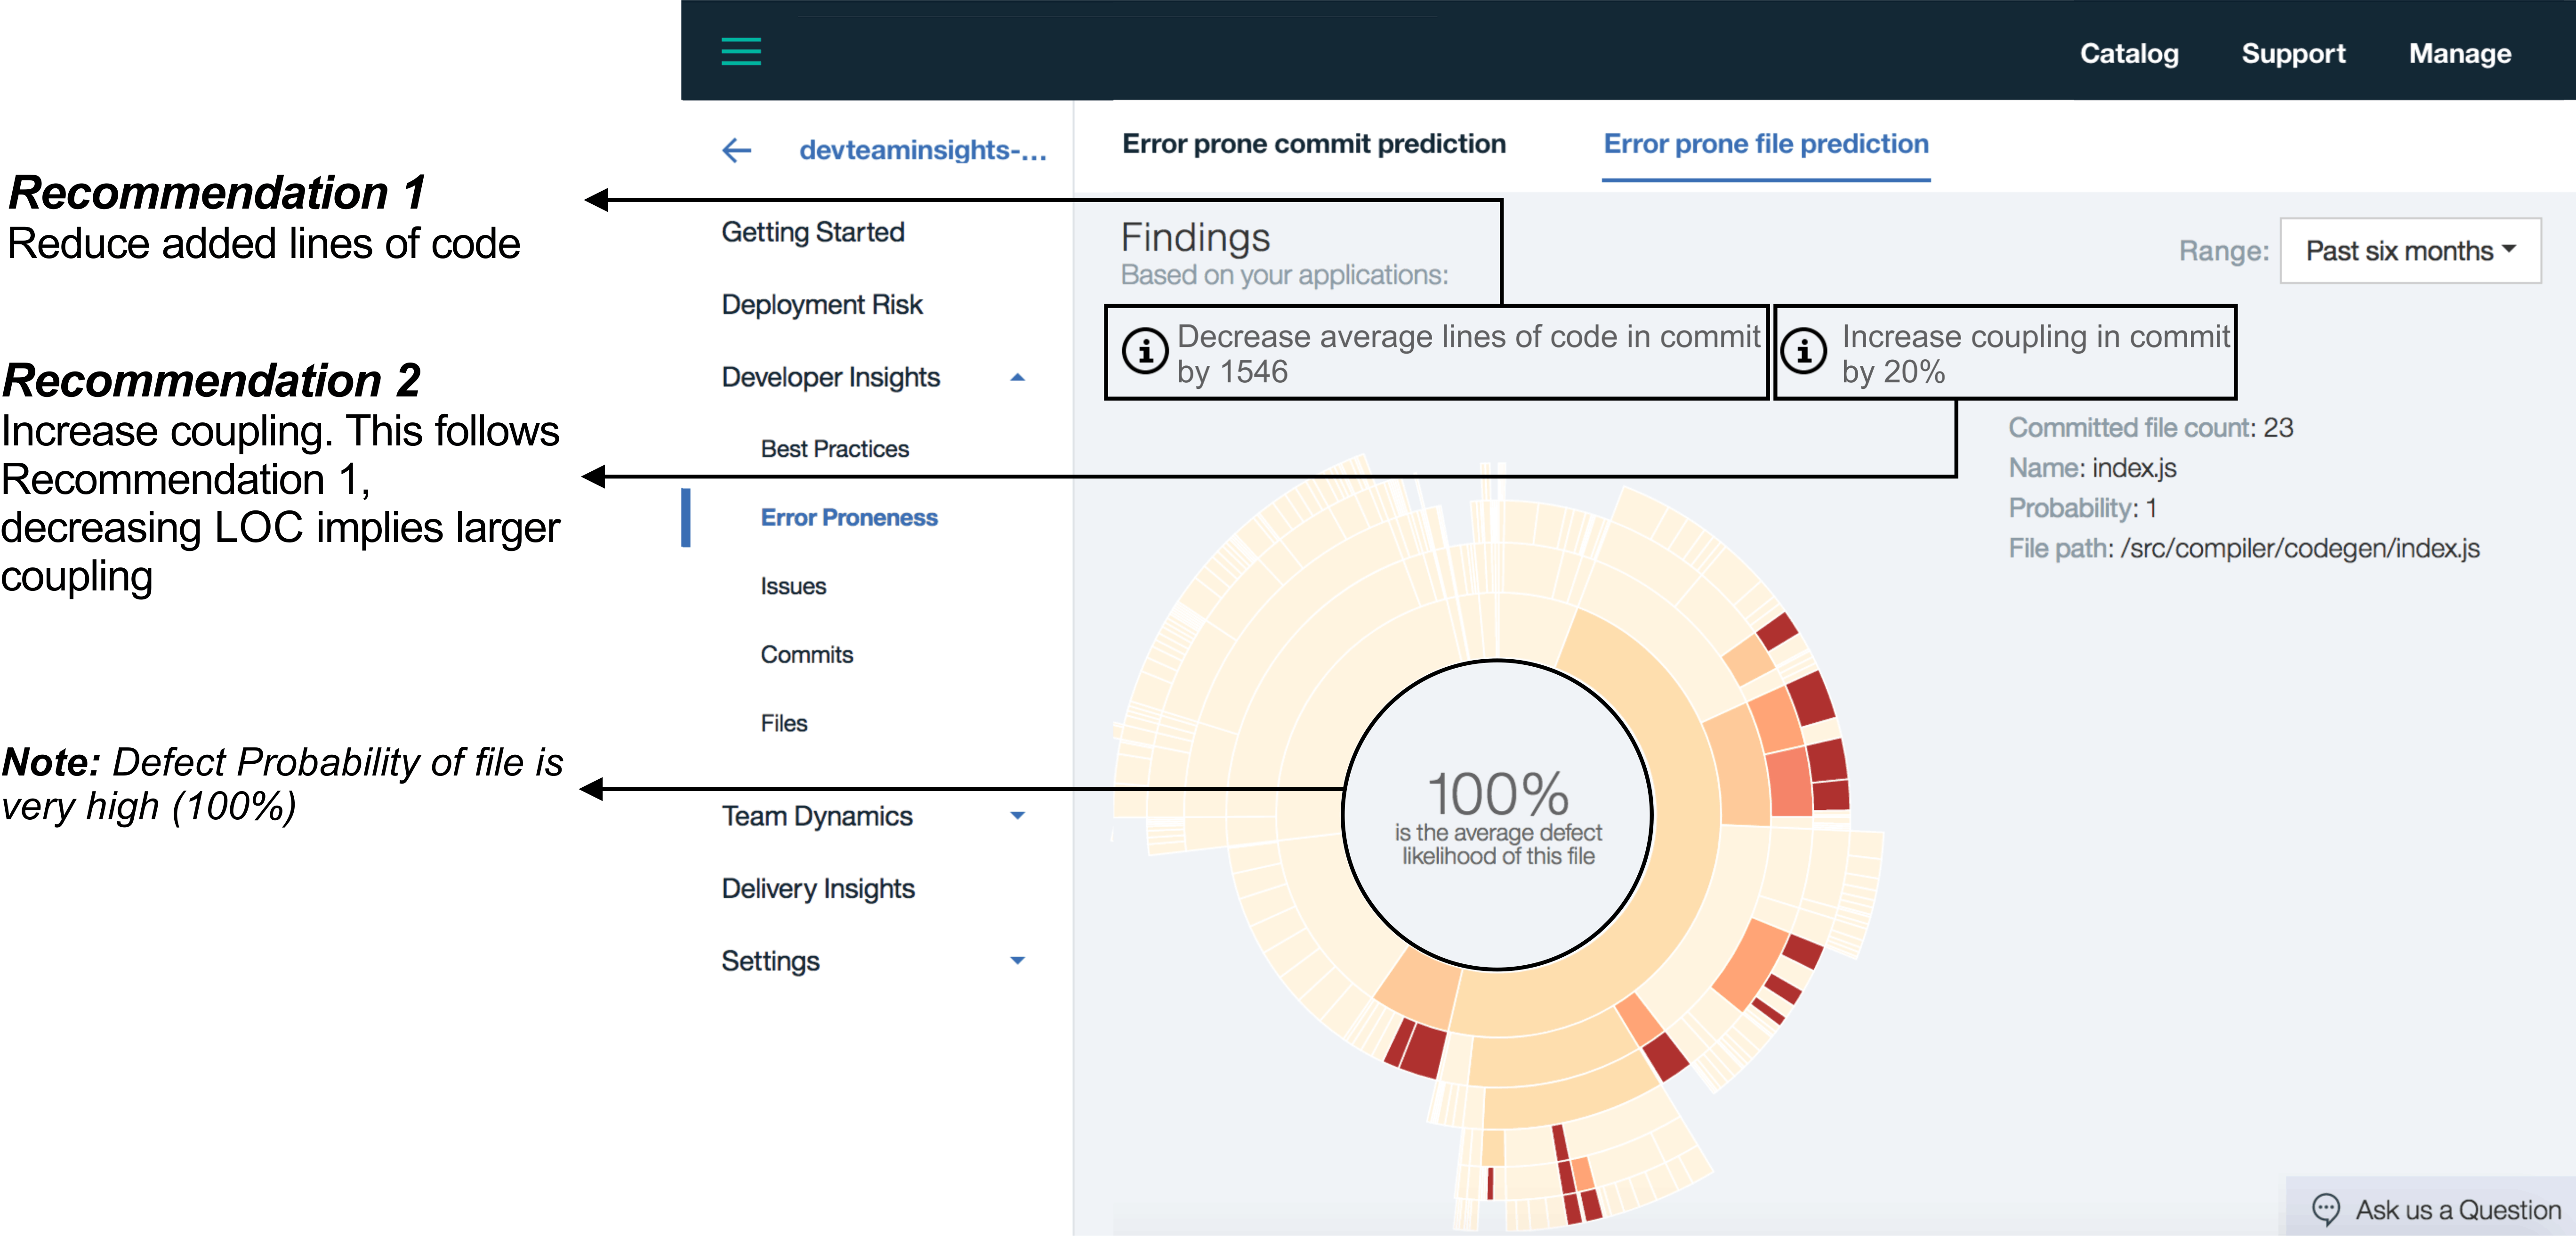
\includegraphics[width=\linewidth]{figs/bluemix.png}
    \caption{The CrossTREEs tools used in this research has already been deployed into
   a cloud-based programmer IDE. The circular display shows lines of ode in a software system
    and the red sections denote regions predicted to be buggy. The recommendations shown on the screen are CrossTREEs' advice
    for how a developer can reduce the expected number of bugs
    in their code. By our reckoning, screens like the above are seen
    by the developers of 1600 projects. Given all that expertise reflecting on our recommendations, the research challenge of this research it so find some way to combine all the insight into better and actionable models of
    software quality
}
    \label{fig:bluemix}
\end{figure}




% %   Note that   CrossTREE  satisfies   the above    principles of knowledge elicitation discussed in {\bf \S{4a}}:
% %   \bi
% %   \item
% %   \mbox{{\em Principle \#1:}}
% % CrossTREE's recommendations are not dense richly-connected models. Rather, they read
% % like LTM fragments; i.e. tiny context-specific knowledge fragments that offer specific advice what to do in specific situations. 
% % \item
% % \mbox{{\em Principle \#2:}}, CrossTREE can be used for ``knowledge elicitation via irrigation''.
% %  Instead of asking developers ``what factors increase software project quality?'' we will
% %  instead show developers  CrossTREE recommendations, then track what response that evolves. 
% % Specifically, we will post the recommendation as an issue report. After that,
% %  it will be clear if developers act
% %  on that recommendation 
% %  (i.e. if they accept that issue, then move to close to the issue as ``completed'').
% % Other researchers~\cite{theisen2017risk} report that such a ``post an issue and see what happens'' tactic is an effective experimentation  for  teams communicate extensively via Github issue reports.  
% % \ei 

% % {\bf 4c. Knowledge combination + PSO:} If we believed that there is no value in human insight, then our current
% % systems, which generates recommendations like \fig{bluemix}, would suffice.  However, our goal is to
% % test {\em combinations}
% % of human and artificial intelligence. Therefore, more machinery is required.

% % This  section describes our PSO architecture.  
% % We use PSO since it is a  {\em socio-cognitive} approach where
% %  all inference is made by jostling around
% % all the  opinions of other members of the community.
% % This makes it a natural method for exploring a space of possible contradictory opinions, only some of which might   actually be useful
% % for improving quality.





% % % Recalling {\bf \S{2}}, our premise is that any assertion from humans or from an AI might  sometimes be wrong.
% % % Hence, we cannot uncritically accept any such assertion. Instead, we must create an arena 
% % % where novel extensions to old ideas must compete to demonstrate their value (and ideas that lose that compete will be purged). Note that this arena should always be reviewing old conclusions since, as we saw above
% % % in \mbox{{\bf \S{2a}}}, one problem
% % % with SE knowledge is that SE developers fixate on old patterns while rarely revising them.


% % % Within that arena, we will run a multi-objective optimizers to solve the above  four goal multi-objective problems
% % % i.e. minimize $(I,O)$ while maximizing $(E,D_i)$.
% % % To build that arena, we will use the  particle swarm optimization (PSO)~\cite{Eb95} algorithm
% % % where  particle contains one {\em planning association rule}
% % %  The details of PSO are discussed below, after some technical notes on planning association rules.
 
 
% %  Over the past several decades researchers have reported that stochastic algorithms (e.g. PSO, genetic algorithms) can 
% %  generate very effective rule sets~\cite{Gold85, dejong90, dejon93, vent93,va92}. These stochastic methods have been applied to such diverse domains such as mining rules for credit assignment~\cite{grefen, grefenstette93} and for learning very complex first order logic rules~\cite{Aug95}. Of particular interest to us is the finding that this approach is particularly useful for combining rules derived from expert opinion with machine derived rules~\cite{Ish97}. For
% %  example, stochastic algorithms can also be extended to synthesize expert opinion with fuzzy control rules~\cite{he98}.
% % A distinct advantage of generating rules from stochastic algorithms is that it enables discovering a few interesting, high-level prediction rules from the databases, rather than discovering  a large rule set as was the usual practice with other approaches~\cite{Fr98}. Further, using evolutionary algorithms, these rules can also be derived from streaming data without much overhead ~\cite{Vi11}.


% % For our domains,  rules will take the  form {\em LHS $\rightarrow$ RHS} where $\mathit{LHS} \cap \mathit{RHS}=\emptyset$
% %  and {\em LHS,RHS} are sets of attribute ranges taken from the project data (we create these ranges using
% %  the methods described below).
% %  Each rule is a plan that should be following in a certain context and can be interpreted
% %  as ``when the LHS is true, change the ranges to the values seen in the RHS''. 
 

 


% % % \begin{wrapfigure}[15]{R}{0.4\textwidth}
% 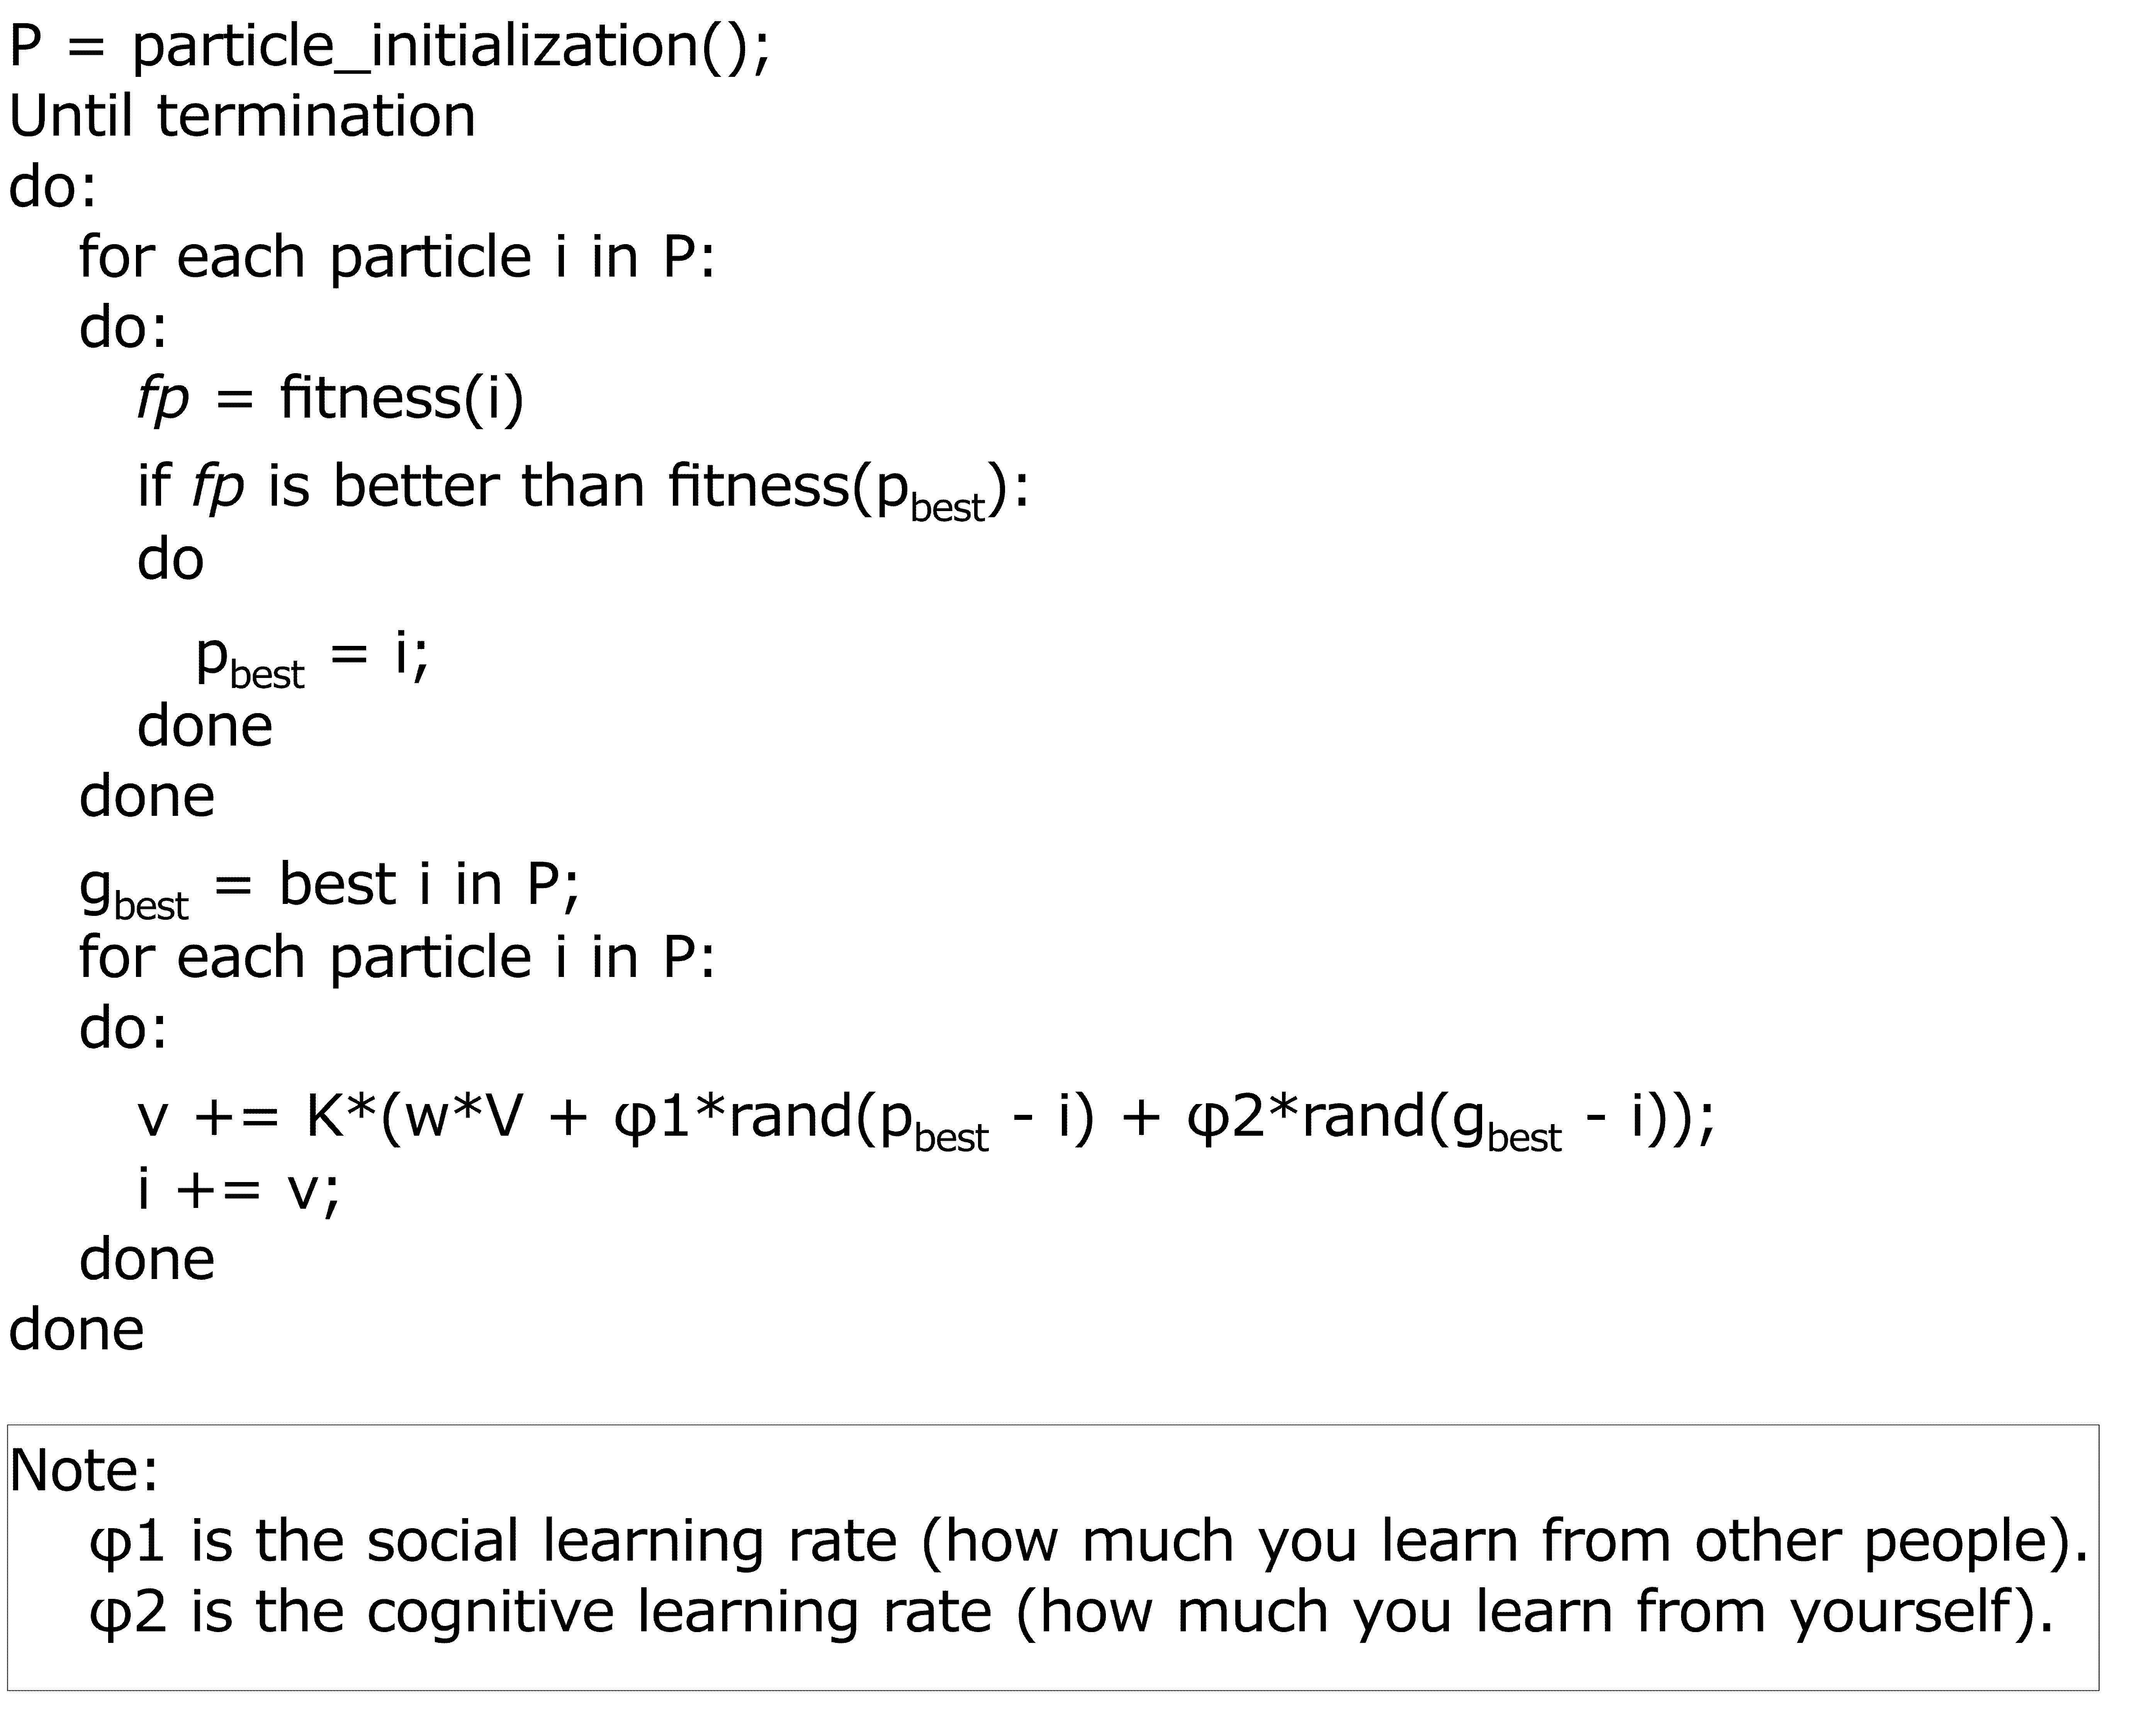
\includegraphics[width=\linewidth]{figs/pso_pseudo.png}
% \caption{Pseudocode for a basic PSO.}
% \label{fig:pso_pseudo}
% \end{wrapfigure}

\begin{figure}[!b]
\begin{minipage}{0.5\linewidth}
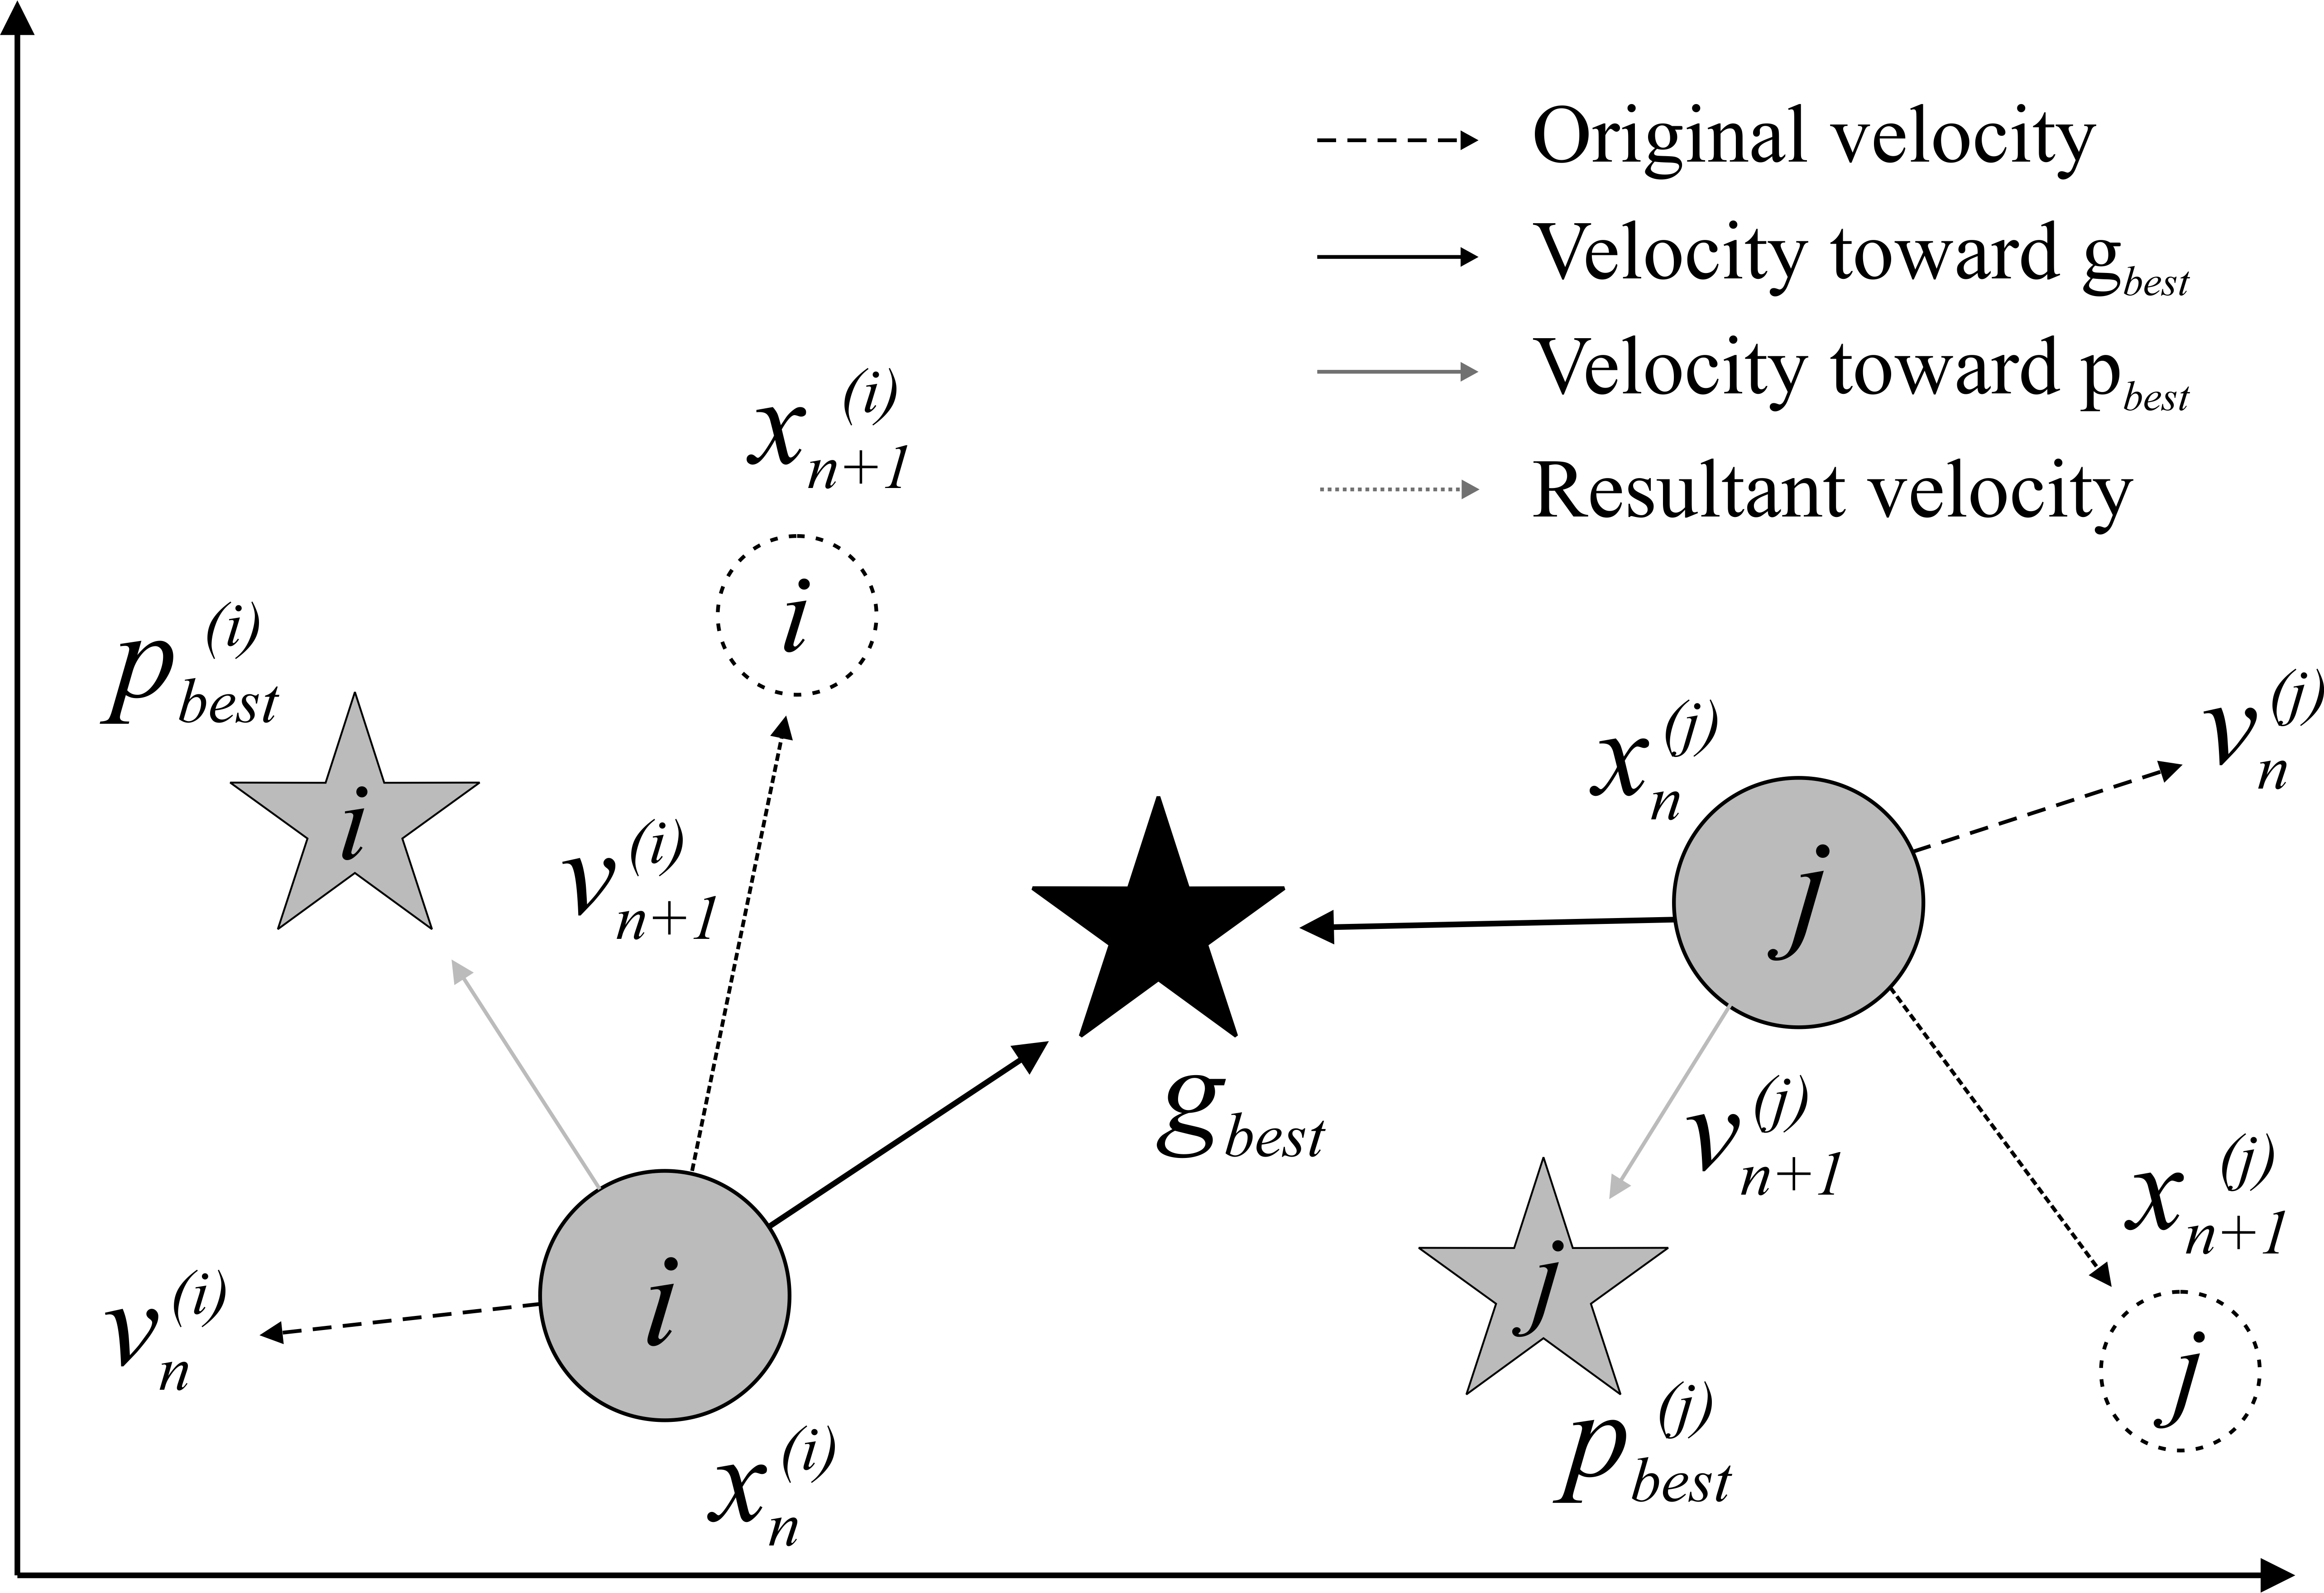
\includegraphics[width=\linewidth]{figs/pso_demo.png}
\caption{Mutations in PSO.}
\label{fig:pso}
\end{minipage}~~~~\begin{minipage}{0.5\linewidth}
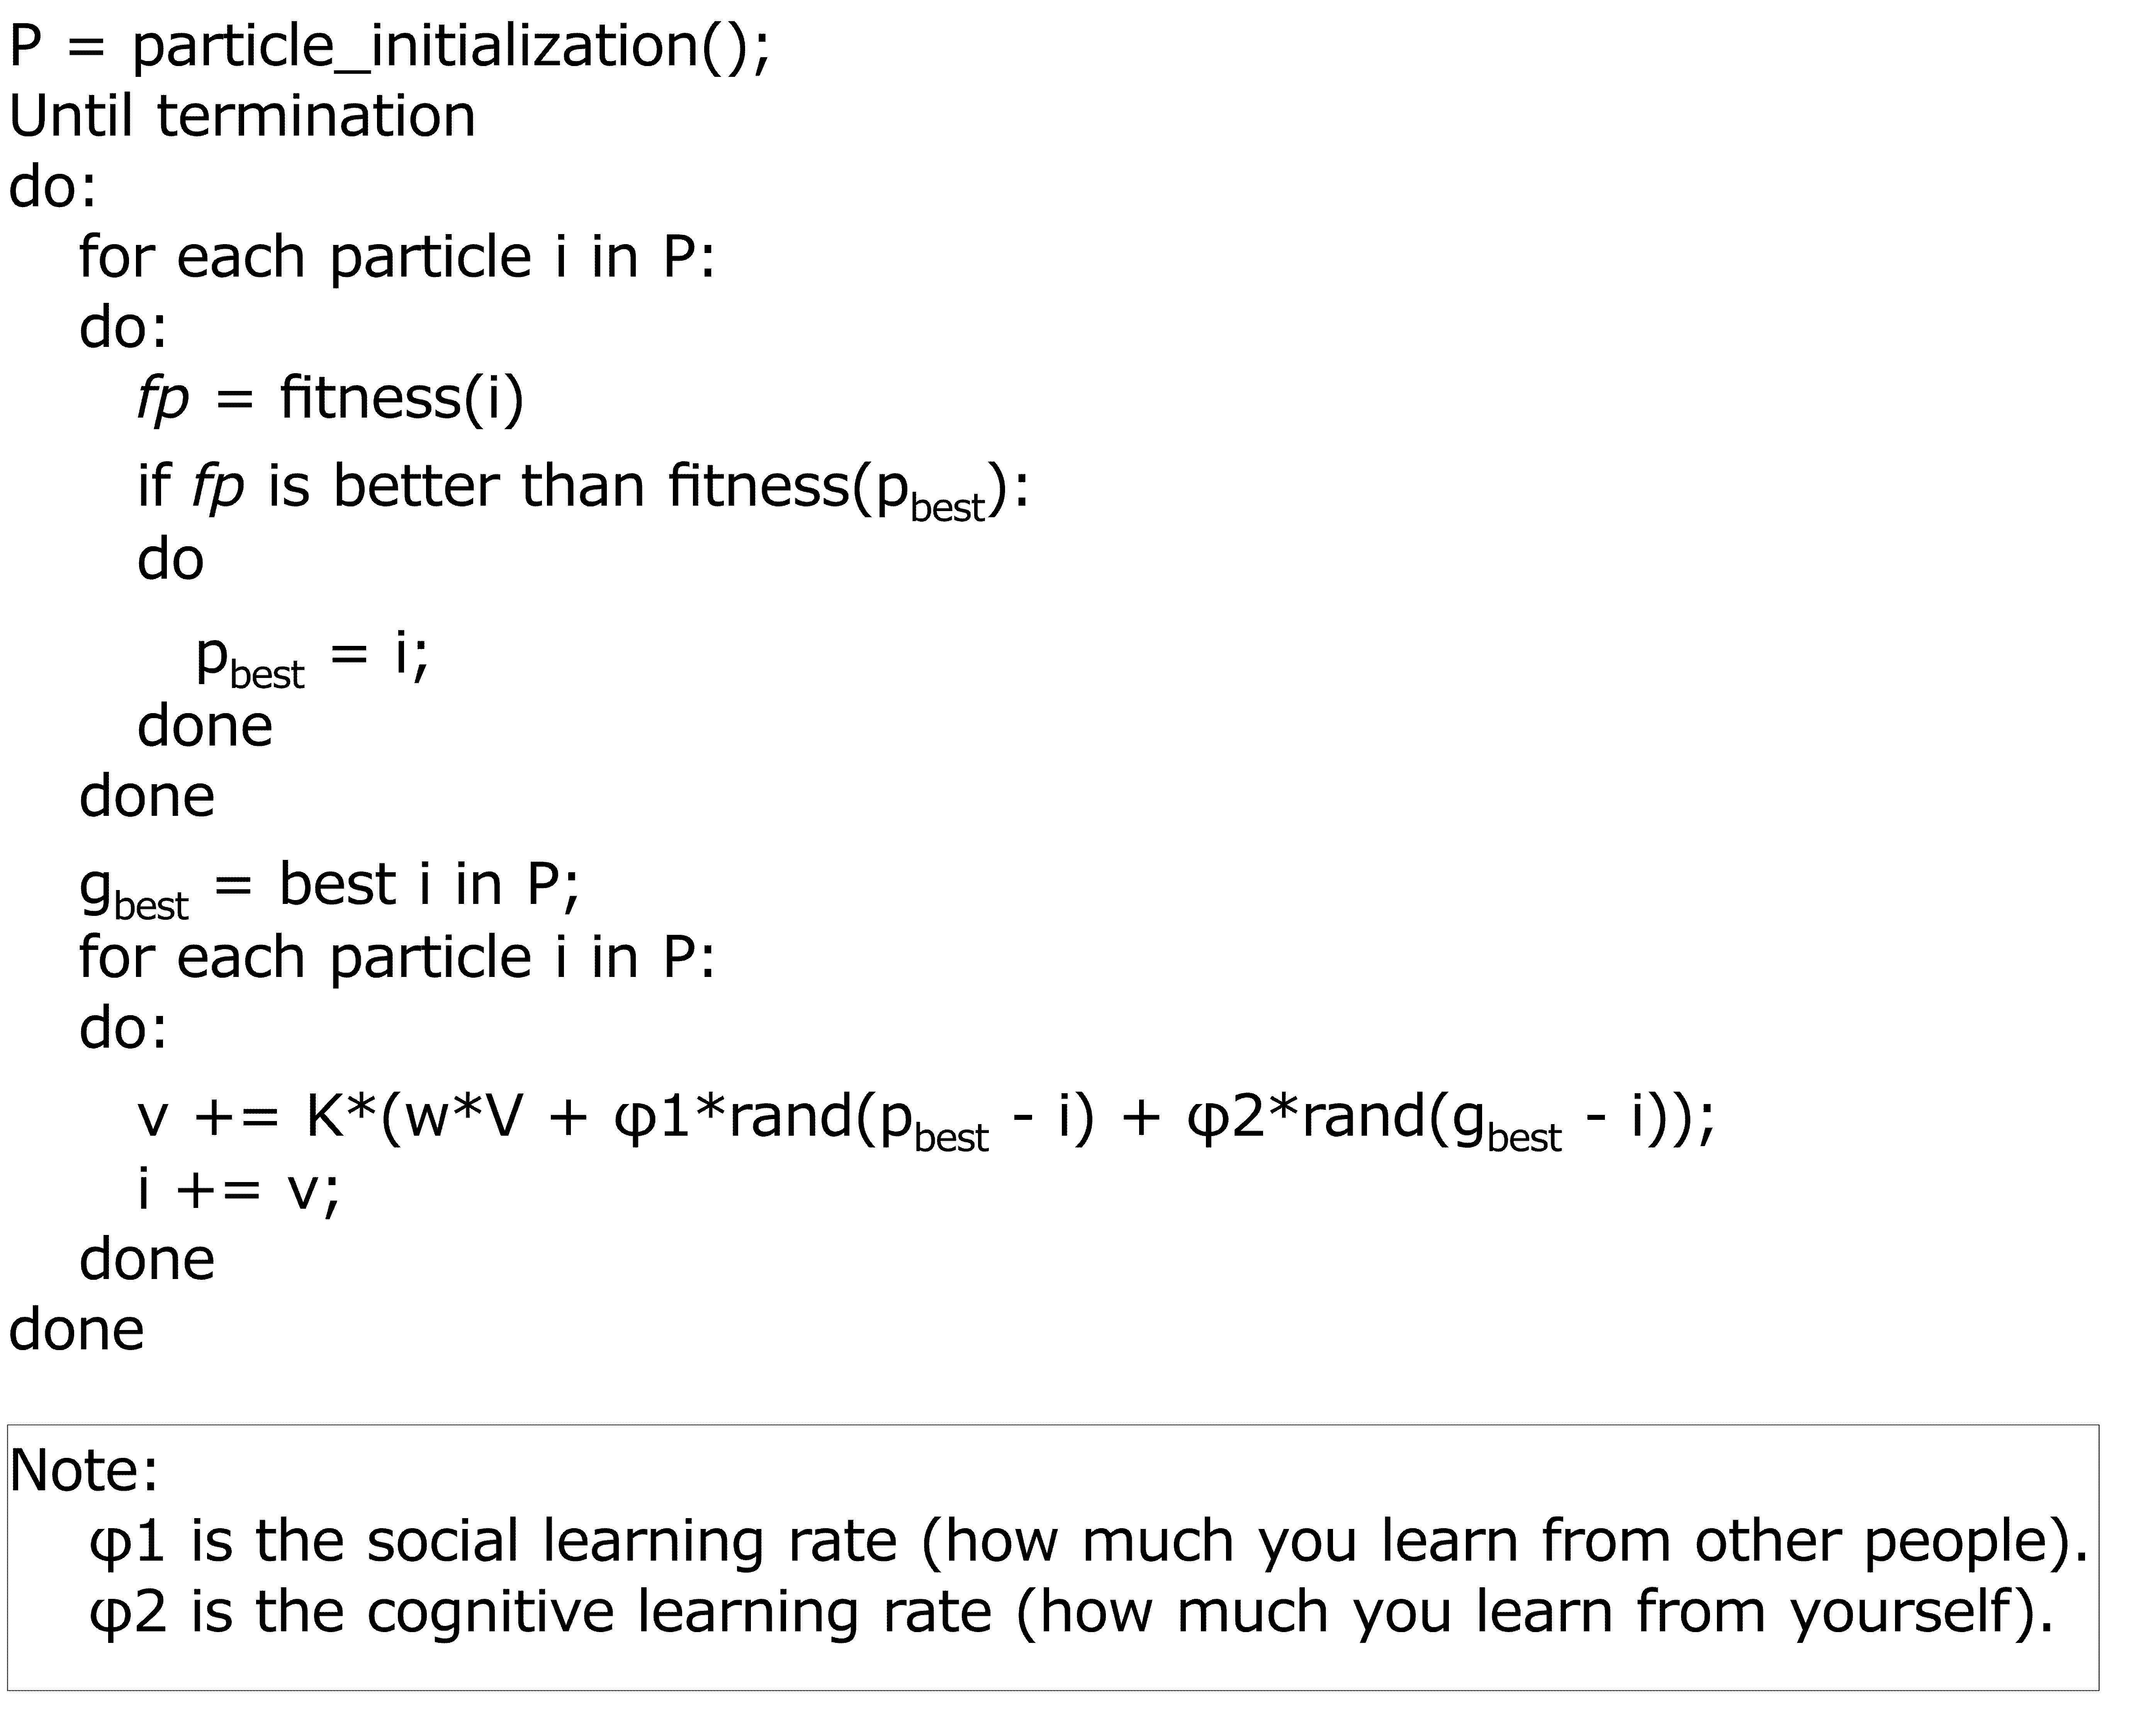
\includegraphics[width=\linewidth]{figs/pso_pseudo.png}
\caption{Pseudocode for a basic PSO.}
\label{fig:pso_pseudo}
\end{minipage}
\end{figure}

% \begin{wrapfigure}[15]{R}{0.4\textwidth}
% 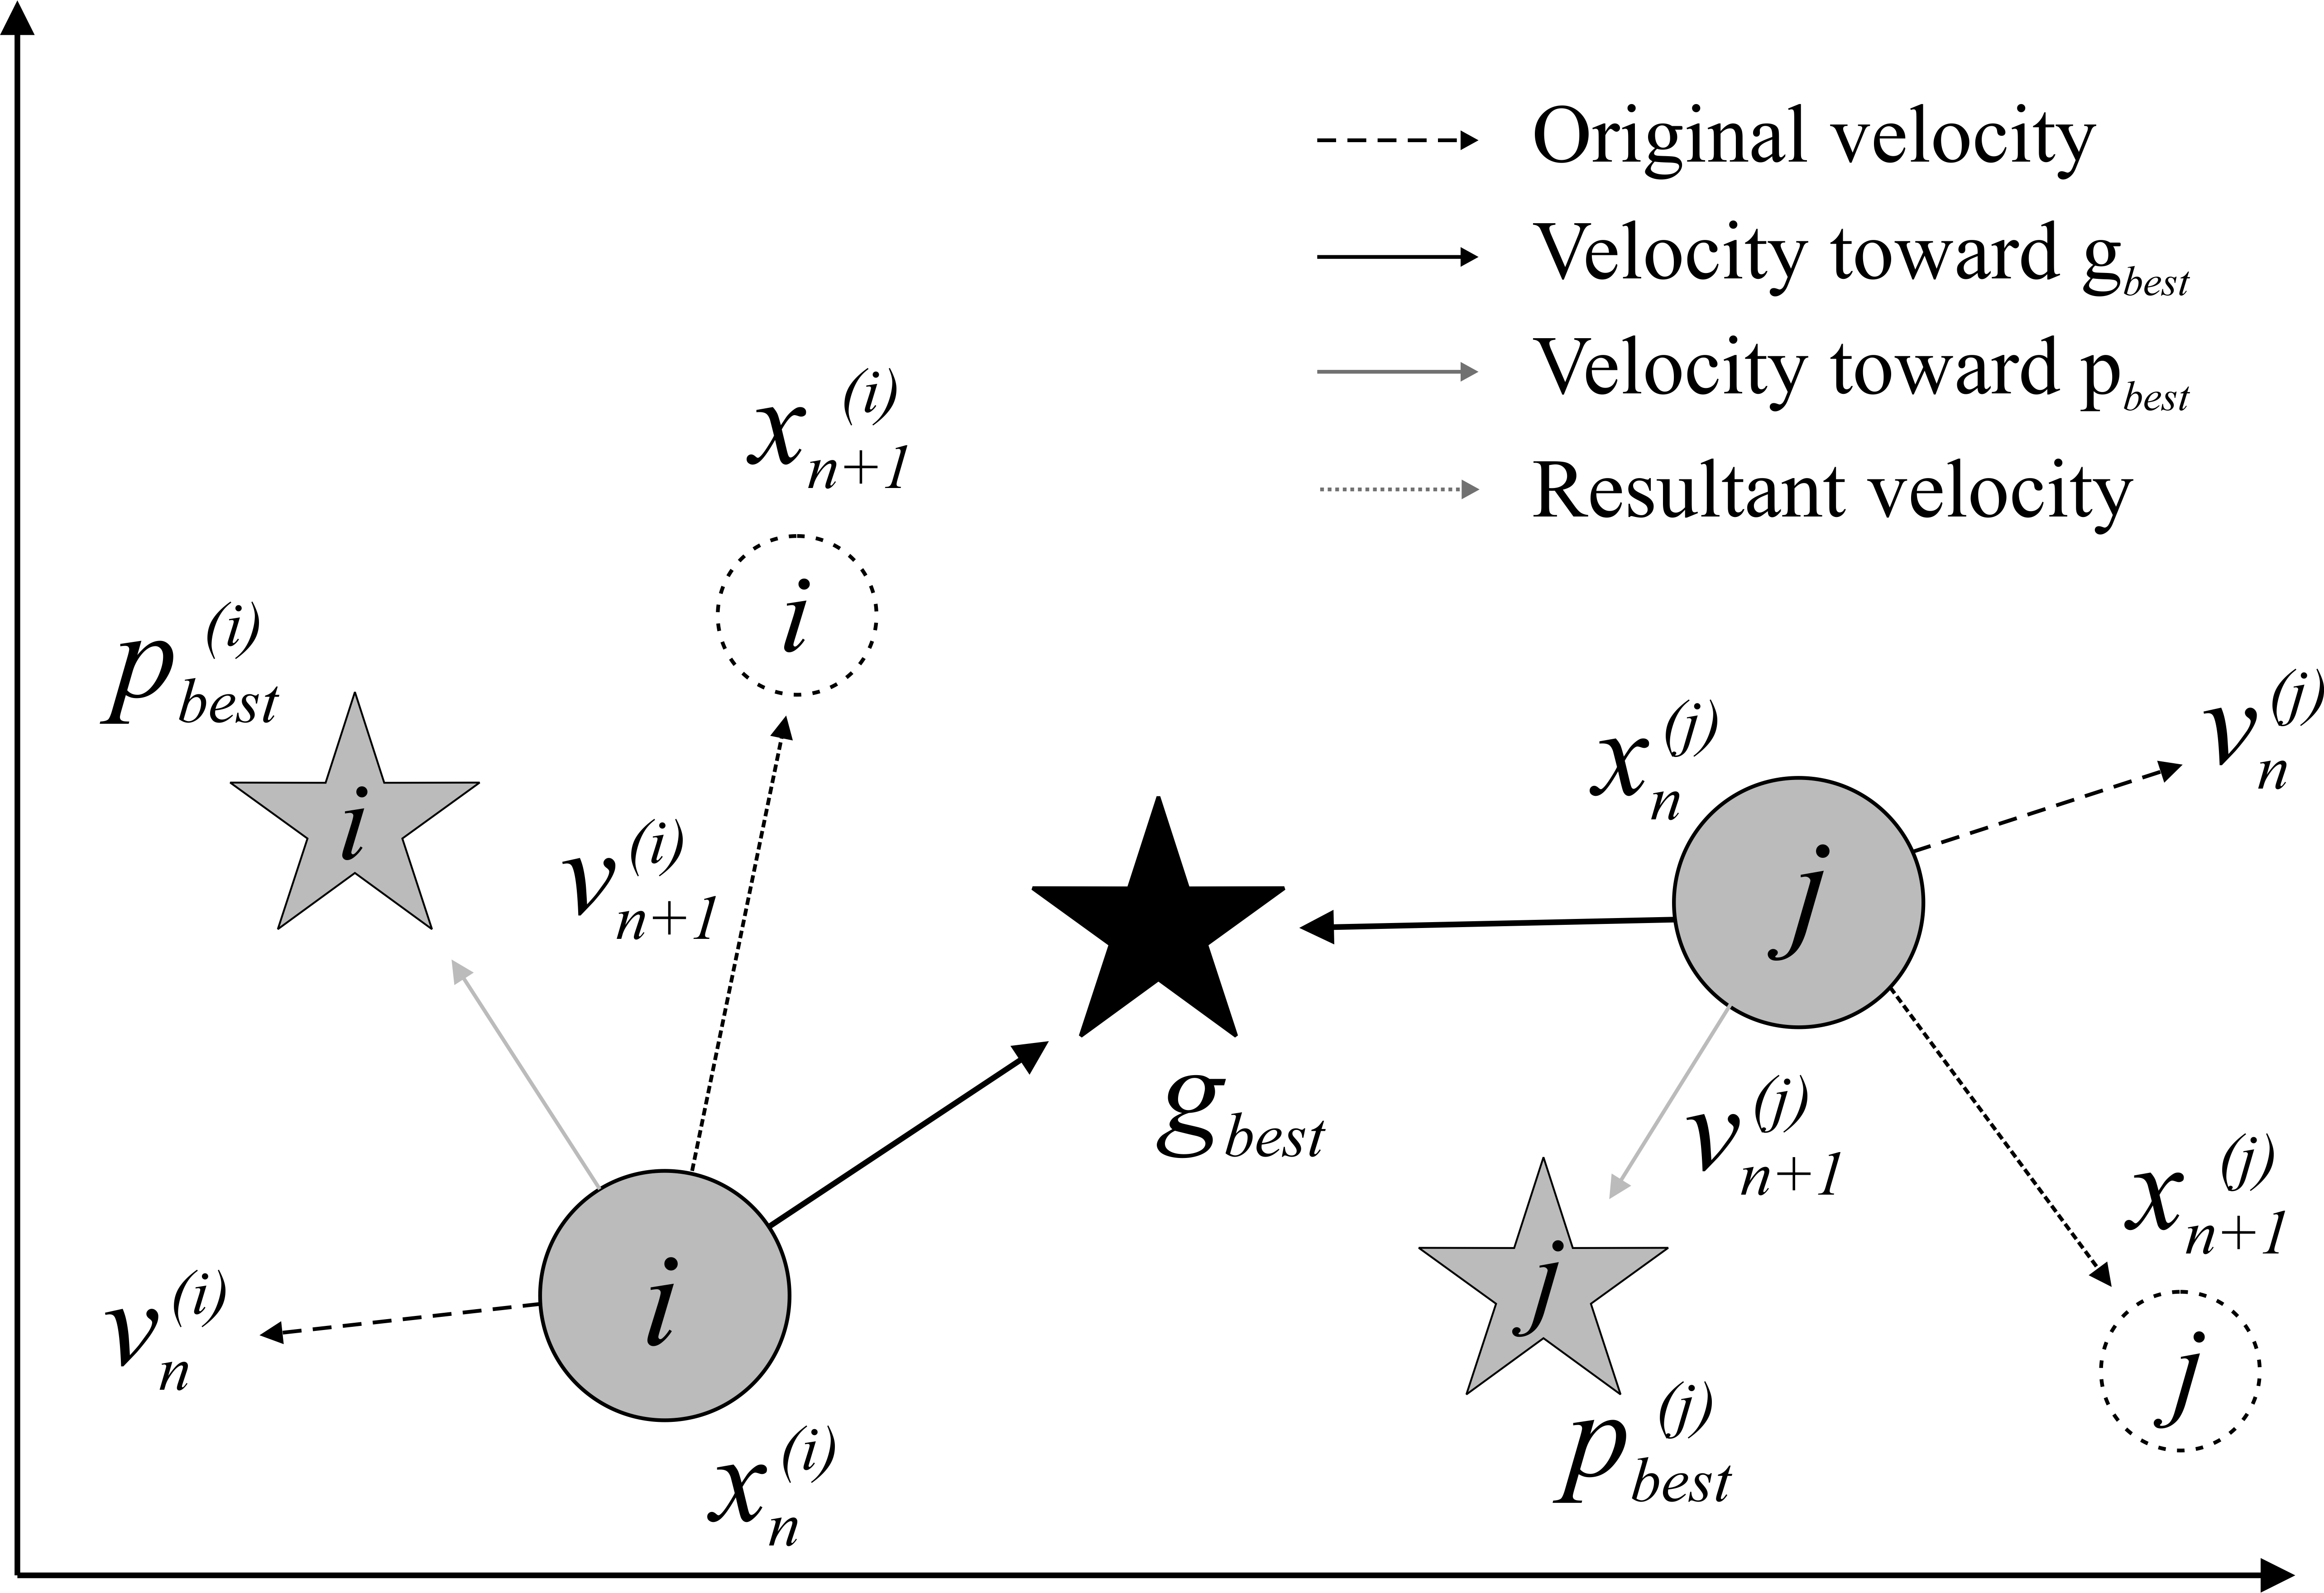
\includegraphics[width=\linewidth]{figs/pso_demo.png}
% \caption{PSO uses sociocognition to mutate its particles. Each particle $i$  mutates in the direction
% $v_n^{(i)}$ while also pulled towards
% (1)~the best idea it ever saw in the past $p_{\mathit{best}}^{(i)}$
% as well as (2)~the best idea ever seen by the community 
% $g_{\mathit{best}}$. As a result, the particle $i$ is redirected towards $x_{n+1}^{i}$.}
% \label{fig:pso}
% \end{wrapfigure}



% % Our intent is to use stochastic algorithms to learn rules that satisfy the optimization problem described in {\bf \S{3}}.
% % As to the mutation method, referring to \fig{pso},
% % each particle $i$  in the swam has
% % its current mutation  direction
% % $v_n^{(i)}$. That particle is   also being pulled towards
% % (i)~the best rule it ever saw in the past $p_{\mathit{best}}^{(i)}$
% % as well as (ii)~the best rule ever seen by the community 
% % $g_{\mathit{best}}$ (this best rule is marked by ``{\LARGE $\star$}'' in \fig{pso}. 
% % As shown in \fig{pso_pseudo}, the pull is determined by  a social cognition factor  $\phi_1$
% % (that controls how much we learn from others) and
% %  a cognitive learning rate $\phi_2$ (that controls how much we learn from ourselves).
% % As a result, the particle $i$ is redirected towards $x_{n+1}^{i}$. For further technical details on our PSO approach, see \tab{arch}:

% % \begin{table}[!t]
% % % \footnotesize
% % \caption{To apply PSO to planning association rules, we need to define (A)~what is a particle; (B)~how to determine when one solution is {\em better than} another; (C)~{\em direction of mutation} of a rule;
% % and (D)~how to nudge the direction by adding in another rule. }\label{tab:arch}
% % { 
% % \begin{tabular}{|p{.99\linewidth}|}\hline

% % {\em (A) What is a particle?}
% % A particle  holds two planning association rules: {\em current} (which is being actively mutated) and  {\em best} which is a copy of the best current planning rule seen so far.
% %  Particles
% % also hold a list of sorted ranges, described below. At each step of the SWARM, the current rule is mutated using   ``direction of mutation'' (shown below).
% % \\\hline


% % {\em (B)~When is one rule better than another?}  This question is answered by a {\em domination predicate} that reports
% % one item in a multi-objective space is better than another. More precisely, we define ``better'' via  using Zitler's indicator
% % dominance predicate~\cite{zitzler2004indicator} that says rule
% %   $x$   is better than rule  
% %   $y$ if  
% %   $M(y,x) > M(x,y)$
% %   where \mbox{$M(x,y) = \sum_j^n -e^{\Delta(j,x,y,n)}/n$}
% %  and \mbox{$\Delta(j,x,y,n)  =  w_j(o_{j,x}  - o_{j,y})/n$}.
% % In these expressions,
% %  $w\in \{-1,1\}$   represents the $n$ objectives that need to be minimized or maximized. Also, 
% %  $o_x, o_y$ are the objective scores associated with $x,y$; i.e. the 
% %   $(o_x,o_y)\in\{I,O,E,D_i\}$ goals from {\bf \S{3}}.
% % \\\hline
% % {\em (C)~What is a rule's ``direction of mutation''?}
% % Rules mutate in the direction defined by weights on a list of ranges.  
% % Given a set of records, we  compute the {\em domination count}; i.e. using the Zitler predicate, for each records $x$ count how many record $y$ are dominated by  this row.
% % Next, we discretize  the numeric values in those records by   (a) sorting the values then (b) recursively finding the splits that minimizing the expected value of the standard deviation of the domination count (using the  CART feature selection rule~\cite{breiman1984classification}).

% % ~~~~ Each   symbolic range and discretized numeric range is then weighted. Ranges are selected stochastically as follows.
% % Compute the CDF (cumulative distribution function) for all the ranges, sorted by those
% %  weights. 
% %  For $A$ attributes, add   $A$  ranges to a rule via  a binary search over the range CDF looking for the
% %  range/attribute pair associated with the   random number $0 \le R \le W$.

% % ~~~~This search will select between $0$ to $A$
% % ranges for each attribute (so attributes whose ranges are all ranked lowly will rarely be selected). Attributes that are not selected by this process are not
% % added to a particles {\em current rule}.   Attributes with more than 1 selected range become   disjunctions. 
% % Clearly, this  CDF search will tend to select attribute ranges from the ranges with largest weights. 
% %  \\\hline
% % {\em (D)~How to nudge the direction by adding in another direction?}
% % To nudge the mutation direction of   rule, we compute the weighted sum of the range weights from two rules (and if a range is in one rule, but not the other, then it has a weight of zero). As seen in \fig{pso_pseudo}, that combination is controlled by the variables  $K,~\phi_1,~\phi_2$
% % where 
% % $K$ is a constriction factor to damp escalating velocities; and
% %  $\phi_1,\phi_2$ control the relative
% % weightings given to the locally and globally known best solution.
% % Carlisle \& Dozier~\cite{An01}    $\phi_1$ = 2.8; \mbox{$\phi_2$ = 1.3} (i.e. listen to your own experience about twice as much as that of your fellows).
% % \\\hline
% % \end{tabular}}

% % \end{table}
 
% % \head{5. RESEARCH PLAN}
% % In the above we motivated a two-part architecture: (a)~CrossTREE to generate a set of (possibly good) recommendations; then (b)~PSO to take advantage of patterns of usage in how
% %  developers use the CrossTREE recommendations. 
% %  This section describes our plan for using this architecture to test the core    hypothesis of this work; i.e.
% % \begin{center}
% %  {\em RQ1:  Are human-augmented data miners ``better'' for software   analytics?}
% %  \end{center}
 
 
% % \noindent
% % {\bf Task0: Evangelizing } {\em (a.k.a. Beating the drum.)}

% % Recalling the discussion around \fig{venn}, we will use feedback from live projects to tune
% % our learning methods. To gather that feedback, we will see what changes result from posting recommendations
% % from CrossTREE into the Github issue tracking system.

% % Other researchers~\cite{theisen2017risk} report that such a ``post an issue and see what happens'' tactic is an effective experimentation  for  teams that communicate via Github issue reports. Nevertheless, it would be prundent to   evangelize our work within the software developer community since, if that were done, developers
% % might look twice at issues   posted from some source called ``CrossTREE quality system''.

% % We anticipate no difficulties in visiting local software organizations
% % and evangelizing this project to a very large local population. It turns out that at NC State University, evangelizing to a large developer community is particularly
% % easy. NC State University is located 20 minutes away from Research Triangle Park (RTP),
% % home to 
% % numerous organizations engaged in extensive software
% % development including
% % (a)~SAS,   (b)~NetApp, (c)~EMC Corporation, (d)~Credit Suisse First Boston,  
% % (e)~the second largest IBM operation 
% % in the world (smaller only than the one in India)
% % with 11,000  local employees
% % and (f)~Cisco Systems' largest campus outside of
% % Silicon Valley with 5380 employees.  Also, nearby is the corporate headquarters
% % of Red Hat software,  Lexis Nexis' national   Technology Center, and the ABB Research Center. 
% % % All these organizations make extensive use of a similar
% % % tool stack (Github, Jira,   Travis CI) and the standard languages seen in 
% % % the continuous operations ecosystem (Java,Node.js,  Go, PHP,  Swift,  Python,  Ruby  Sinatra, Ruby on Rails). 
% % % This convergence of technologies has lead to the emergence of a new generation tools with wide application to
% % % many software projects. For example, the cloud platform used in this research (and shown
% % % in \fig{bluemix} is built and maintained  by one of the organizations listed above.
% % % PI Menzies already has  extensive contacts with that community and,
% % % in the period 2015 to 2017,   received  \$325K in gift money from these organizations
% % % to work on  their software analytics projects. 
% % % PI Menzies regularly publishes papers with  research-active members of that industrial community;
% % % e.g. see ~\cite{krishna2016bigse,yu16} and the two ICSE SEIP'18 submissions currently under development.  
% % % % More importantly:
% % % \bi
% % % \item Many students from NC State take jobs in the local software industry;
% % % \item
% % % Four of PI Menzies'  Ph.D. students students work as interns with these organizations-- and
% % % two of those students work 
% % % directly with the team maintaining the cloud platform used for this work.
% % % \ei
 
% % \noindent
% % {\bf Task1: Sanity checks} {\em (a.k.a. The best thing to do with some data is throw it away.)}


% % % \begin{figure}[!b]
    \centering
    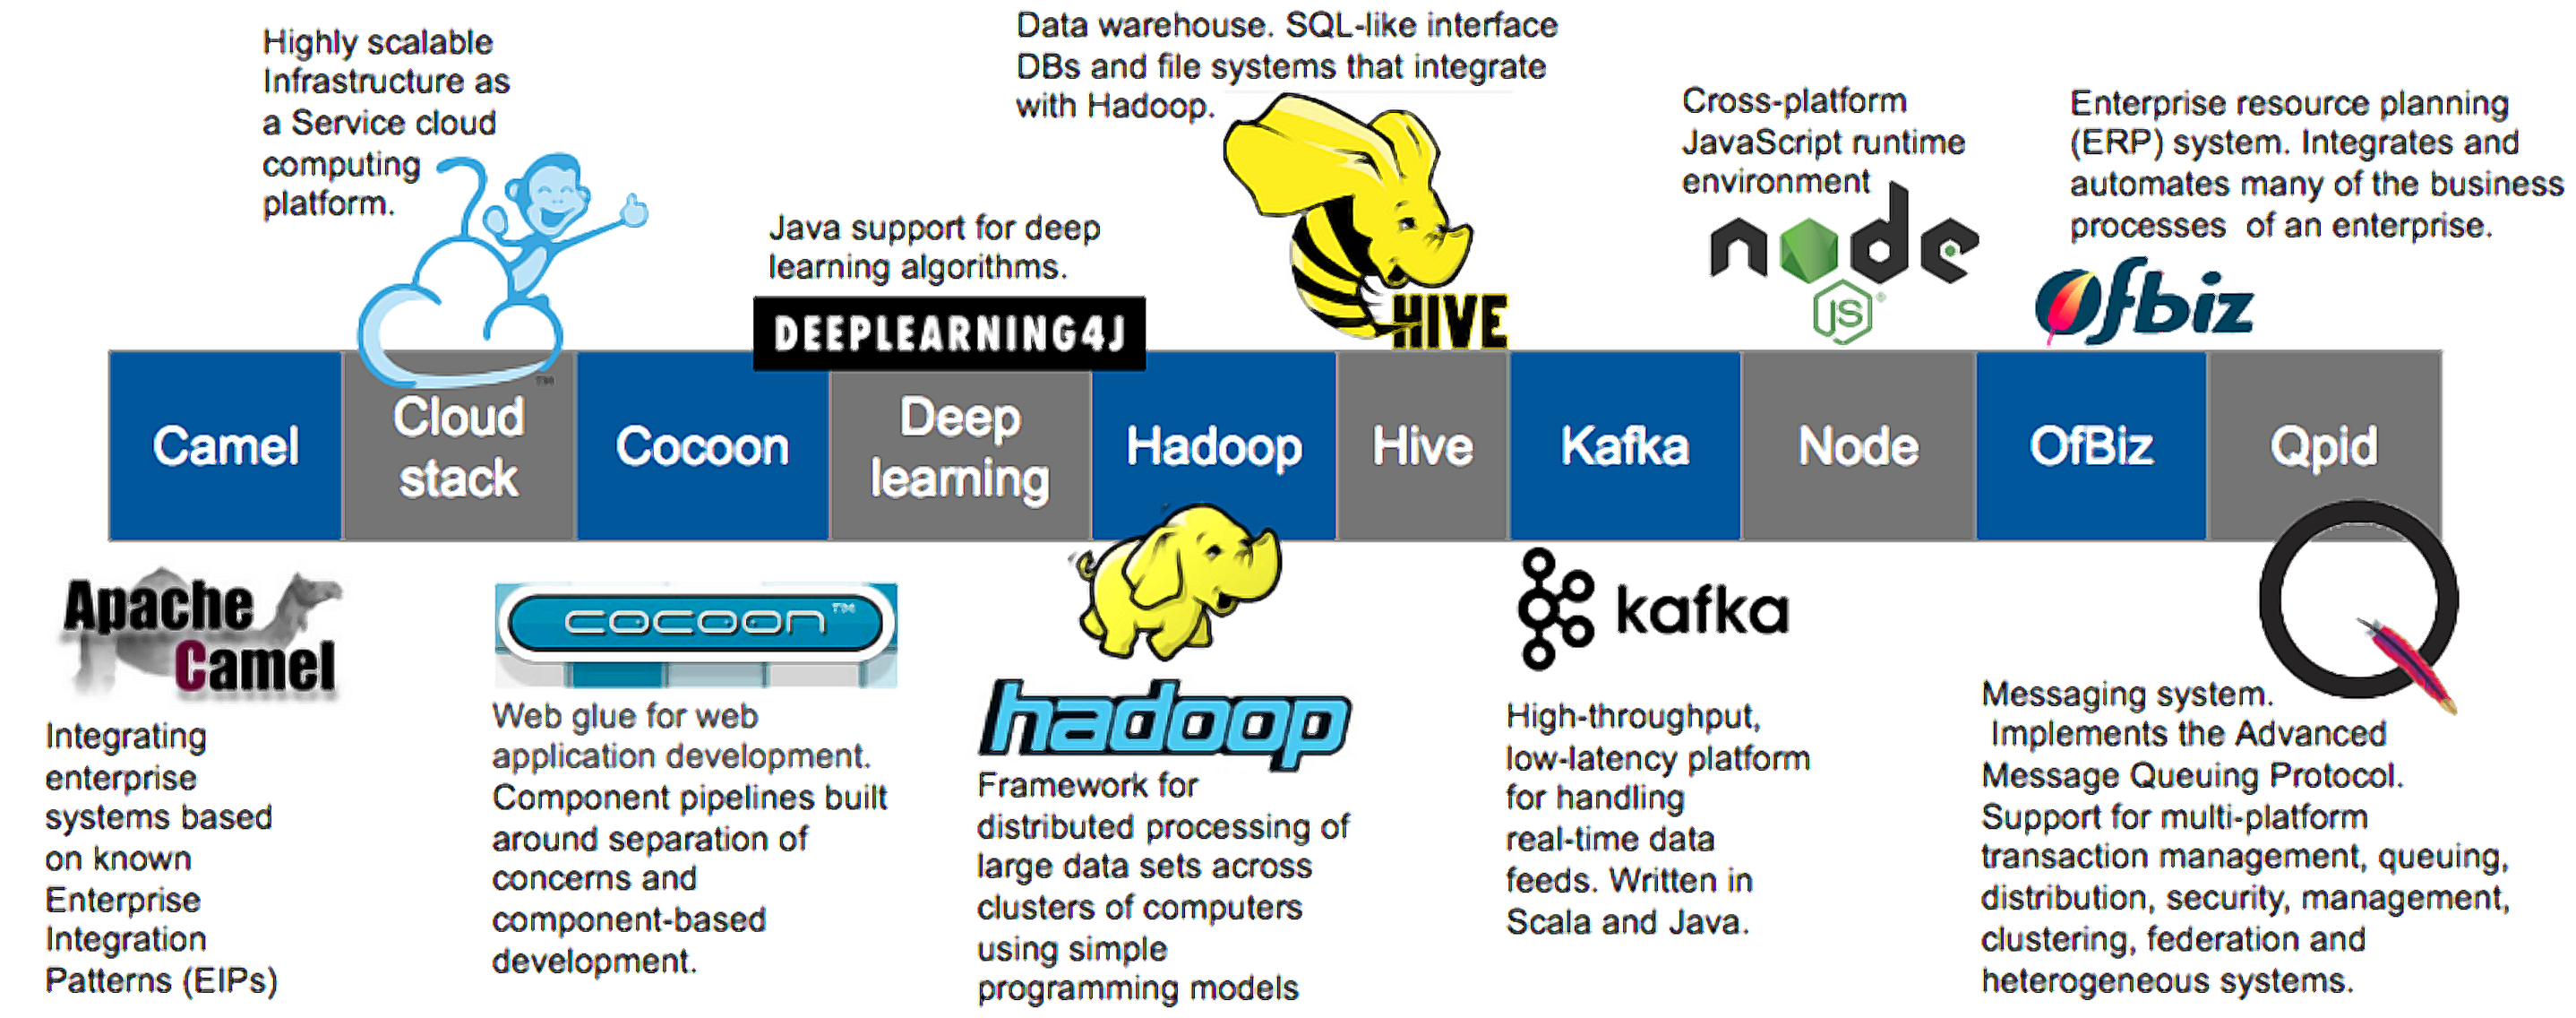
\includegraphics[width=\linewidth]{figs/projects.png}
    \caption{This project will use data from many open source projects, including the above.}
    \label{fig:projects}
\end{figure}


% % The cloud platform used 
% % for this work has already ingested Github/ Jira/ Travis CI  data from
% % 538 in-house projects.
% % and over 1100 open-source projects
% % marked by Github as ``most trending''. A small sample of those projects are listed in \fig{flow}
% %  (and note that, for confidentiality reasons,
% % we cannot list details on the proprietary projects we can access within this cloud platform).
 

% % Bird et al.~\cite{bird2009promises} caution that many  Github projects are mere ``hobby'' projects and these should not be used as part of any serious research project.
% % They offer a list of ``sanity checks'' for selecting Github projects. Based on experience with this  data, we have slightly
% % augmented those sanity checks. \tab{sanity} shows the results of applying those sanity checks to our 1646 projects. Note that even after culling ``hobby''
% % projects, we are still left with hundreds of open source and in-house projects to use in this research.
 

% % \begin{wraptable}[13]{r!}{0.6\textwidth}
\footnotesize
\centering
\caption{Sanity checks. Starting with 1108+538  open source+in-house projects, we discard  projects that {\em fail}
any of the LHS tests to arrive at 661+171 projects.}\label{tab:sanity}
\begin{tabular}{|l|r|r|}
\hline
Sanity check & \multicolumn{2}{c|}{\#discarded projects}                     \\ \cline{2-3} 
\multicolumn{1}{|c|}{(discard projects that violate these tests) }                              & \multicolumn{1}{l|}{In-house} & \multicolumn{1}{l|}{Open-source} \\ \hline
\# Pulls \textgreater 0                             & 35                            & 54                              \\
\# Issues \textgreater 10                            & 60                            & 89                              \\
\# Commits \textgreater 20                          & 68                            & 96                              \\
\# Developers \textgreater 8                        & 47                            & 67                              \\
\# Releases \textgreater 0                          & 136                           & 44                              \\
Project time frame \textgreater 1 year              & 12                            & 46                              \\
Projects doing only software development            & 9                             & 51                              \\ \hline
%Total Projects                                      & 538                           & 1108                            \\
Surviving projects                                  & 171                           & 661                             \\ \hline
\end{tabular}
\end{wraptable} As to other data cleansing tasks, we will perform {\em column pruning} via the range generation method of \tab{arch} (part C),
% % and {\em outlier removal} via the clustering methods described below in {\bf Task3}.


 
% % \noindent
% % {\bf Task2: Goal Stratification} {\em (a.k.a. We cannot do everything, but we want to do many things.)}
 
% %  Recall from  {\bf \S{3}} that  the goals of this work are to learn software quality plans that minimize $I,O$ and maximize $E,G_x$. 
% % As shown in \tab{metrics},
% % our data set supports
% % exploration of many external attributes, any one of which could be the quality goal $G_x$ we will seek to maximize.
% % % That said, the  data we are exploring is   vast and the patterns of \fig{venn} are only meaningful if developers are changing code
% % % in order to achieve some goal that they actually care about.
% % % Hence, for this work, we will restrict our search for software quality goals $G_x$ for
% % % which it is known that some   manager or developer or active research
% % % group is currently exploring. 

% % % It turns out, even with that restriction, there are many such quality issues.
% % For the last two years, 
% % PI Menzies and his graduate students have  regularly interviewed studies with project
% % managers and developers to find the issues that drive their policy decisions.
% % and how those goals can be assessed via data mined from tools like Github, Jira, Travis CI, etc. 
% % In these sessions, we asked managers and developers ``what do you want to do, and do better?''. Their answers are as follows.
% % In this first task we will hold extensive on-line surveys   and in-person meetings to check the currency of the above list, perhaps to even expand it.
% % \bi
% % \item[$G_1=$]
% % Reduce defects~\cite{moniruzzaman2013comparative}; 
% % \item[$G_2=$]
% % Decrease development effort~\cite{sarro2016multi,menzies2017negative}; 
% % \item[$G_3=$]
% % Reduce issue resolution time~\cite{rees2017better}; 
% % \item[$G_4=$]
% % Rank issues such that more important ones get resolved faster than more trivial problems~\cite{moniruzzaman2013comparative}; 
% % \item[$G_5=$]
% % Decrease the impact of new personnel to project productivity~\cite{brooks1975mythical}, e.g. by learning a threshold below which it is safe to add new programmers to a project~\cite{agrawal17time};
% % \item[$G_6=$]
% % Increase the use of less-expensive software tools that improve productivity~\cite{bruckhaus1996impact}, or decrease the use of expensive tools that have no discernible
% % effect on products~\cite{rahman2014comparing}; 
% % \item[$G_7=$] Providing a proper documentation so that new personnel joining can have reduced ramp up time~\cite{petersen2009comparison}.
% % \item[$G_8=$]
% % Assess if it is useful to adopt a Continuous Integration approach~\cite{shahin2017continuous,vasilescu2015quality}.
% % \item[$G_9=$]
% % Determine what are the  right rate of releases for a project. 
% % If too slow  then a vendor might lose their customer base (customers may jump to other vendors offering more novel functionality
% % faster)~\cite{chen2015continuous}.
% % \item[$G_{10}=$] Provide techniques that can make software development be more language-agnostic~\cite{mens2005challenges}.
% % \item[$G_{11}=$]
% % Discover the right time for adding personnel to a project. If removed too early then the current project will suffer. If removed too late then too many programmers will be working on 
% % current projects (and newer work will be unnecessarily delayed)~\cite{rodriguez2012empirical}.
% % \item[$G_{12}=$]
% % Learn different ``bad smells''. For e.g.,
% %     \bi
% %         \item[$G_{12a}=$] Program features that are usually associated with code problems.
% %         \item[$G_{12b}=$] Process features that are usually associated with late or otherwise challenged projects. Further, an example of this might be a team  where most of the changes are (a)~made by a few  ``hero'' programmers~\cite{agrawal17hero} or (b) novice developers are likely to introduce defects than those produced by subject matter experts.
% %     \ei
% % \ei
% % There are two encouraging aspects to the above list. Fristly, 
% % we already have preliminary results on some of the above (see references to our work at $G_3,G_5, G_{12}$).  
% % That is, we already know that which data source is a rich source of insight into software engineering.
% % % \item
% % % We have discussed this list with several industrial cloud-based development teams. While not all goals are interesting
% % % to all parties, there is much overlap in their current interests.
% % Secondly, 
% % Many of these goals are also active research areas in the literature (see all those with references). For those
% % goals we will have ready access to alternate methods (and results from those methods) which we can use to baseline
% % our results. Also, the presence of those other research results means that we have a publication path for this work
% % (e.g. ``previously, a team at ABC argued for DEF but using our human-augmented data mining approach we have discovered GHI'').


% % \noindent
% % {\bf Task3: Data Stratification} {\em  (a.k.a. Not everything applies to everything. )}
 
% % Another way to divide this problem is {\em data stratification}. Boehm~\cite{Boehm:2006} strongly
% % advocates for data stratifications; i.e. not learning on all available data but on targeted subsets.
% % % A similar conclusion comes from other researchers~\cite{menzies2013guest} including Krishna et al.'s  who comments that
% % % during   transfer learning  (using data from one project to learn predictors for another)
% % %  if data
% % % is divided N ways, then best results for one division come from a poll across (a small number) of nearby divisions~\cite{Me13,krishna2017learning}. 
% % % There are many ways to divide SE data, some of which are not always productive. For example:
% % % \bi
% % % \item
% % % Dividing software project data via implementation language is becoming less and less useful since many current
% % % projects now use combinations of languages for different parts of their system.
% % % \item
% % % Dividing data into
% % % open source and proprietary is not always helpful. With Agrawal~\cite{agrawal17hero}, we have found that many 
% % % of our quality measures are not statistically significantly different between open source and proprietary.
% % % Further, with He et al.~\cite{he13} note that,  after computing the distance between projects (measured as an aggregate
% % % over the data from these different projects),   (a)~some proprietary projects are in fact closer to open source 
% % % projects that other proprietary projects and (b)~best quality estimates for open source projects can sometimes
% % % come from proprietary projects.
% % % \ei
% % Some such stratifications can  be very useful. 
% % % For example, Agrawal~\cite{agrawal17hero}  reports that if projects
% % % are sorted via frequency of release, then there are very clear divisions between waterfall-style projects
% % % (which release rarely) and agile-style projects (that release very frequently). 
% % Petersen and Wohlin~\cite{Petersen2009} have commented on which context variables to explore when searching through project data.
% % While we plan to follow their advice wherever possible, their advice has two limits. First, they offer certain pre-defined stratifications for software projects and there is no way for a reader of that work to determine if those stratifications are more useful than some other set. Secondly, given the ever-changing nature of the software landscape, it is likely that new kinds of projects
% % will appear in the near future. Petersen and Wohlin are silent on how to commission new kinds of stratifications.

% % Previously we have much success with automatic stratification tools. Such automatic clustering
% % address our two issues with the Petersen and Wohlin manual clustering approach.
% % When  clusters are learned automatically,   new kinds of projects are always accommodated;
% % Also, 
% % such clusters are always auto-assessed via the clustering creation mechanisms.

% % The are many other advantages to such auto-clustering.
% % Firstly, an important data cleansing heuristic is {\em outlier removal}; i.e. only do the reasoning within
% % similar sets of records. Clustering implements this important data cleansing step since, for each cluster, every other cluster is the outlier.
% % % Secondly, the rules generated from local clusters
% % % contain more effects familiar to developers working on projects in those clusters.
% % Secondly,
% % if data is stratified automatically via clustering algorithms,
% % then the resulting models learned per cluster may have similar median performance but
% % have far less variance than models learned from all the data~\cite{Me13}. 
% % % Fourthly, During 
% % % {\em transfer learning} (where data from one project is used to make predictions for another), then
% % % some subset of those clusters are often an {\em bellwether} (source of exemplar data that applies to other projects)~\cite{krishna2017learning,krishna2017simpler}. 
% % Thirdly, and
% % more specifically for this project, such automatically-generated clusters can be used to better define the ``global'' best rule as used by the PSO algorithm defined above. Classic PSO use a global ``best'' from all data. But for data as large as what we are processing, it seems prudent to cluster and redefine ``global'' to be mean ``best within the current cluster''.  Hence, for this work, we propose (a)~running
% % some incremental clustering algorithm (e.g. mini-batch K-means~\cite{Sculley:2010}, or its
% % more recent variants ~\cite{Sculley:2010}); then (b)~  running one of our PSO algorithms within each cluster (so in those clusters ``global best'' means ``best in this clster'').
% % One advantage in restricting PSO to subsets of the data is scalability. Whatever the runtime costs of PSO, by dividing that up and running
% % in parallel over multiple
% % tiny regions of data, then this would lead to dramatic speed ups in PSO.

% % \noindent
% % {\bf Task4: Data-lite} {\em (a.k.a. Make it run locally.)}

% % Our initial plan is to make all the above work within the cloud IDE
% % described in the introduction. That said, for the purposes of micro-experimentation and reproducability,
% % it would also be useful to perform all the above outside that IDE.

% % Working outside that IDE is practical and possible. While researchers would lose access to the proprietary projects inside this IDE, they could still access via Github, and associated tools
% % such as  GhTorrent (ghtorrent.org), and 
% % Github Archive (https://www.githubarchive.org/) to access much of the information stored in our
% % cloud platform. However,  are two caveats to that statement. Firstly,
% % the cloud platform offers extensive access to on-line CPU farms and cloud-based secondary storiage devices; and secondly 
% % the cloud platform routinely implements extensive joins between Github and other tools  such as the
% % Jira issue tracking system. Further, the results of those joins are cached and indexed
% % and made available via APIs. 
% % Hence, not everything we could do inside the cloud IDE might be 
% % easily reproducable otherwise. 

% % That said, we suspect it possible that after some experience with
% % our kinds of analysis, there will emerge a ``typical set'' of attributes that most often appear in our
% % planning rules. If such a ``typical set'' is found, then some lightweight collection policies
% % could be added to projects to collect and cache those sets-- in which case it may well be possible
% % to optimize for all the goals we are exploring in the cloud IDE without requiring extensive
% % extensive and expensive cloud-based CPU or secondary storage facilities.

% % \noindent
% % {\bf Task5: Execution} {\em  (a.k.a. Ready, set go.)}

% % Once the data is (a)~cleansed, (b)~sorted into groups reflecting different goals (with spurious records removed), and 
% % (c)~clustered into groups of records, the next task is to:
% % \bi
% % \item
% % Run CrossTREE;
% % \item
% % Which generate recommendations which are posted as issues to developer issue systems;
% % \item
% % Then monitor the subsequent changes to the code base;
% % \ei
% % Note that one of the reasons we are requesting four years of funding for this work is that, since this task will require
% % extensive monitoring to future changes in a project, this task will take some
% % time to complete.

% % \noindent
% % {\bf Task6: Evaluation } {\em (a.k.a. Testing {\bf RQ1}.)}

% % The evaluation criteria for this work was presented above: it was a four-goal optimization problem with the aim
% % to propose changes that were rarely in the sets $I,O$ (things {\em ignored} by developers, or changes {\em other} than
% % what was found by our methods) and were often seen in $E$ (things suggested by our tools and {\em endorsed} and enacted
% % upon by developers) and which had a large beneficial effect on some quality goal $G_x$.
% % Also, for quality goals that other researchers have explored, we would need to see which of those techniques
% % we can reproduce and compare with our methods. For example, in recent work where we built predictors for how Github issues
% % will take to close (using data from the cloud IDE). In our report on that work~\cite{rees2017better}, we showed
% % that our methods out-performed the prior state-of-the-art in this area~\cite{Kikas:2016}.
% % Note that with results from our approach, compared to some prior state-of-the-art, we can test our hypothesis that human-augmented data mining methods produce better predictors and planners for software quality. 
% % \bi
% % \item For a list of prior results relating to our goals, see the citations in the $G_x$ list shown in {\bf Task2}.
% % \ei
% % % The following two results would be very challenging to our research themes:
% % % \bi
% % % \item Methods taken from prior results perform better than our CrossTREE/PSO methods. Such a result would cast doubt on the value of our entire archicture.
% % % \item CrossTREE's recommendations perform just as well as anything generated via PSO. This would tell us that added human intelligence to our artifical intelligence
% % % methods was {\em not} useful, at least for the architecture studied here. Note that this result would {\em not} prove that all 
% % % AI was better than human intelligence (Shull et al.~\cite{shull02} offered examples in his prior work where a little human contextual knowledge greatly improved insight from
% % % automatic tools). But if CrossTREE performs as well as anything else, then it would motivate more resaerch on automatic big data research rather than human-in-the-loop
% % % reasoning.
% % % \ei

% % Other evaluation criteria to be considered are the {\em CPU cost} of our methods.
% % Many of our recent papers~\cite{chen2017beyond,fu2017easy,nair2017faster,mathew2017shorter,nair2017flash,chen2017riot}, 
% % and the work of others~\cite{Fisher:2012}, raises concerns about the reliance on CPU-intensive methods.
% % Such methods complicate reproducability -- an essential part of the scientific methods. Our design, described above, proposes
% % limiting PSO to just clusters found via min0batch K-means.
% % Still,  given the large size of of the data set on
% % the cloud IDE, much of our time will be spend matching information over
% % the data sets. At this time it is unknown if a one-pass summarization
% % algorithm can sweep over the data to return the small amounts of information
% % required for our rule-based reasoning. This issue  must be closely monitored.

% % Finally, another evaluation criteria must be the {\em disk  storage space}
% % needed for our methods. Initially, we will work within the cloud IDE
% % described in the introduction to this proposal. However, recalling
% % at {\bf Task4}, we need to know the minimal storage required to create an active useful working
% % copy.

% % Note that, in this section, we do not list specific metrics or statistical tests. Since our goals $G_x$ are many varied, we would have to
% % adapt our metrics and statistical methods to the requirements of that $G_x$. To aid that process, we would carefully read prior state-of-the-art
% % results about $G_x$ and, as far as practical, adopt their metrics and statistical methods.


% % \noindent
% % {\bf Task7: Refactor } {\em (a.k.a. Optimize our optimizer)}

% % Based on the above experience, it is highly likely that useful engineering possibilities will become obvious as part of this research.
% % Hence, in our timeline (below), we add two ``refactor'' tasks where we pause after year two and year three of our work to pull down our existing architecture
% % and rebuild a better, faster, version 2.0 and 3.0.
 
% % \head{5. TIMELINE}

% % This work  will take four years to complete, for two reasons.
% % Firstly, recalling the discussion around \fig{venn}, we will use feedback from live projects to tune
% % our learning methods. Such feedback takes time to accumulate (and we aim to accelerate that feedback via
% % the our evangelizing {\bf Tasks0}). Secondly, we aim to explore many of the  $G_x$ goals listed above.
% % Given two students assigned to this work, and based on our recent experience with making conclusions
% % from this space~\cite{agrawal17hero,agrawal17time,rees2017better}:
% % \bi
% % \item
% % We guesstimate that it will
% % take 3 to 6 months to process one goal $G_x$.
% % \item
% % That includes the time required to create the data hooks, perform an initial round of analytics,
% % discuss the results with relevant business users, then write a conference paper on that topic.
% % \ei
% % Note that this will only be possible after we commission our PSO planning rules systems as a backend to
% % the CrossTREE system. Hence, our plan is as follows.


% % %\begin{table}
\caption{Timeline}
\label{tab:timeline}
\begin{center}
\small
\setlength\tabcolsep{5pt}
\begin{tabular}{ |l|l|l|l|l|l|l|l|l|}
  \hline
   & Late 2018 & Early 2019 & Late 2019 & Early 2020 & Late 2020 & Early 2021 & Late 2021 & Early 2022\\
   \hline
   Task 1 & \cellcolor{black!20}build v1.0 &&&&&&&\\
   \hline
   Task 2 & \cellcolor{black!20}build v1.0 &&&&&&&\\
   \hline
   Task 3 & \cellcolor{black!20}build v1.0 &&&&&&&\\
   \hline
   Task 4 &  & & & & \cellcolor{black!20} build v2.0 &&&\\
   \hline
   Task 5 &  & \multicolumn{2}{l|}{\cellcolor{black!20}test single goal} &&&&&\\
   \hline
   Task 6 &  & & \multicolumn{2}{l|}{\cellcolor{black!20}test multi-goal}&& \multicolumn{2}{l|}{\cellcolor{black!20}test multi-goal} & \\
   \hline
   Task 7 &  & & & & \cellcolor{black!20} build v2.0 &&&\cellcolor{black!20} build v3.0\\
   \hline
\end{tabular}
\end{center}
\end{table}



% % Given two graduate students (S1,S2):
% % \bi
% % \item Months 0 to 6: implement the architecture; ie. {\bf Tasks 1,2,3} as described above.
% % \item Months 7 to 12: test the architecture; i.e. {\bf Task5,6} on a single goal (e.g.  for $G_1$ defect prediction).
% % \item Month 13 to 24: stress test the architecture. i.e. repeat   the first year work but this time for multiple goals.
% %          Given the above guesstimate, we anticipate two to six conference/journal submissions about different $G_x$ goals.
         
% % \item Month 25 to 30: pause and build version 2.0; . i.e. explore {\bf Task 4} (the {\em Data-lite} work) and {\bf Task7} (the {\em refactor work}).
% % \item Month 31 to 43: stress test architecture v2.0; repeat the first year work using the new archicture. In this period,
% % we anticipate five to ten conference/journal submissions about different $G_x$ goals.
% % \item Month 44 to 48:    build version 3.0 using {\bf Task4} and {\bf Task7}, and final reports.
% % \ei
% % Note that during all the above steps, our work would always available via public GitHub repositories. Also, as an on-going task,
% % we would be conduct many sessions with local practitioners as part of {\bf Task0} (i.e. {\em evangelizing}). Further, assuming our
% % tool set was mature enough, we would run tutorial sessions at major international conferences (e.g. IEEE ASE) to further evangelize the toolkit.

% % % Based on this architecture, we ask three research questions:
% % % \bi
% % % \item[{\bf RQ1}:] (Baseline question): What kinds of insights can we learn from this data? 
% % % \item[{\bf RQ2}:] (Core question):     Can we learn better insights from   human or automated or human+automated sources? 
% % % \ei
% % % The rest of this section discusses these questions, one by one.

% % % \noindent
% % % {\bf RQ1: (Baseline question): What kinds of insights can we learn from this data? } To answer this question, we need to perform {\em baseline} studies
% % % to discover in what areas our data source supports any insights. We call this the baseline question since, unless we can demonstrate there is any signal
% % % in all the data within our cloud platform, then there is little point continuing.






 


% % %  Note that developers from 1646 projects see these recommendations of \fig{my_label}  on a regular basis. 
% % % Given all that expertise reflecting on our recommendations, there is a tremendous   opportunity here is to research tools
% % % for  combining all that insight into better and actionable models of software quality (hence this research),

% % % % \noindent\texttt{XXX} \\
% % % % \texttt{XXX}


% % % Our proposal is to use an evolutionary program to take rules learned by a data miner, then look at the nouns (and, if any, numeric thresholds) mentioned by humans discussing the rules. Mutation operators would then explore stochastically varying the rules by mutating Boolean operators (and, or, not) or number range queries ($\geq$, $>$, $=$, $!=$, $<$, $\leq$) or the attributes mentioned in the rule.


% % % This research will attempt to answer the following research questions:


% % % \bi

% % % \item \textbf{RQ1: Is human expertise better than data miners?
% % % } A premise of this work is that human intelligence can usefully augment artificially intelligent data miners. Is this even true?


% % % \item  \textbf{RQ2: Will humans ever reach consensus on ``best'' knowledge? }If we ask a community of developers to critique and improve a rule (learned by, say, CrossTREE), will those humans ever reach consensus?


% % % \item \textbf{RQ3: What is the right language for the CrossTREE rules?} Currently CrossTREE works by using static code measures (the object-oriented Chidamber \& Kemerer metrics~\cite{Ch94}). Are these measures useful or are there better measures?

% % % \ei

% % % Accordingly, working with his graduate student Mr. Rahul Krishna, PI Menzies has installed such a ``first pass'' knowledge generator in the software analytics dashboards used by software developers.




% % % \paragraph{\textbf{ISSUE \#1:  Can we trust the current generation of anti-patterns? Can we learn new and better ones?}}

% % % One way to generate critiques is to make use of ``anti-patterns''. According to   Fowler~\cite{fowler99}, anti-patterns (a.k.a. code smells) are ``a surface indication that usually corresponds to a deeper problem''. Fowler  recommends   removing   code smells   by
% % % \begin{quote}
% % % 	``$\ldots$ applying a series of small behavior-preserving 
% % % 	transformations, each of which seem `too small to be worth doing'.
% % % 	The  effect of these refactoring transformations is quite 
% % % 	significant. By doing them in small steps you reduce the risk
% % % 	of introducing errors''.
% % % \end{quote}
	
% % % Several researchers such as Alves, Erni, Hermans, Shatnawi et al.~\cite{Al10},~\cite{Er96},~\cite{He15}, and~\cite{Sh10} static code metrics to propose various formulae as a ``anti-pattern detectors'' e.g. Erni et al. raises a ``anti-pattern'' alert if any static code measure is above  $\mu+\sigma$  for that distribution.  These papers are widely cited\footnote{As of August 2017, Google Scholar reported that the Alves, Erni, Hermans,and Shatnawi's papers have received  118, 116, 23, and  85 citations, respectively.}. But do are these bad smell detectors effective anti-patterns? I.e. can we use them as a guide to avoid problems with the software?  

% % % To test this, we recently compared their recommendations  against our new anti-pattern detector, the CrossTREE contrast learner~\cite{Kr16}.  CrossTREE builds a decision tree (according to the policies shown in~\fig{crosstree}) that predicts for software quality. It then classifies a new project artifact in the usual way by following the branches relevant to the artifact down to some leaf L1 of the tree.  Next, it finds a second leaf L2 such that examples on L2 are more likely to have higher quality than L1. CrossTREE's recommendations on how to change this artifact from bug-prone to bug free is the delta between the branches from the current leaf L1 to  the better leaf L2. For more details on CrossTREE, see top of next page.

% % % CrossTREE  finds deltas to the nearest branch that predicts for higher quality (where ``near'' is measured by number of edges in the branches). This  minimal learning style  is a very different approach to the equational methods that  typically reflect across all software artifact attributes and so many recommend far more changes than CrossTREE. For example, in the  following study,  CrossTREE and the Alves equations usually recommended 4 and 20 changes (respectively) per project artifact.  


% % % CrossTREE, and the equational methods, can be used to guide changes to software; i.e. alter the software such that these equations, or CrossTREE, no longer predict that the code will be buggy. To assess these different methods we used defect logs from open source JAVA projects from the PROMISE\footnote{XXX; url} and SEACRAFT\footnote{XXX: url} repository  as follows:


% % % \be
% % %     \item We used Random Forests\footnote{Random Forests were used since Ghotra and Lessmann et al.~\cite{Gh15},~\cite{Le08} both strongly recommend that algorithm.} to  construct  defect predictors. To ensure this experiment was fair, we kept this test set (used by Random Forests) separate to the training set (used to tune CrossTREE and the equational methods);
% % %     \item Using separate data, we  tuned the equations and CrossTREE  (each tuning was its own experiment);
% % %     \item We applied the changes recommended in step-2 to the code used in step-2;
% % %     \item Using the Random Forests from step-1, we tested how many bugs would be seen if the code was changed using the recommendations of  CrossTREE or the different equations;
% % %     \item Report the percent decrease $D$ in classes predicted to be buggy i.e. $D=100\times(1-\dfrac{v}{u})$ \\Where $u$, $v$ are the percent predicted to be buggy by Random Forests before and after step-3, respectively. CrossTREE and the equational approaches were ranked by how much they reduced bug predictions.  

% % % \ee

% % % \input{tex/CrossTREE.tex}

% % % To guard against spurious effects, the above was repeated 30 times with different randomly selected separate train/test sets. The median and inter-quartile range (IQR) results for  D are shown in~\fig{xtree_results}
% % % % \footnote{In this figure, ``CD'' is an ancestor of XTREE which we no longer recommend (since these results show that its clustering  methods perform very badly).} (and note that larger values of P are better)
% % % . Also, note that the Enri and Hermans et al. methods were not studied here since one has to yet to demonstrate popularity in the literature and the other offered no empirical evidence that its bad smell detector was effective. In those results, we see that one data set (Jedit) was impervious to 
% % % improvement via any method. Otherwise, CrossTREE or Alves performed best (and one widely cited method from Shatnawi  performed very badly indeed).  In summary, these experiments show that just because a bad smell detector is widely cited (e.g the Shatnawi equations), that does not mean we should use those detectors. We now recommend CrossTREE over the equational approaches since (a) as mentioned above, CrossTREE recommended far fewer changes than the Alves method; and (b)  current experimental results show that CrossTREE's recommendations are often as good (or better) than other approaches.

% % % \bi[leftmargin=*]
% % % \item The notion of ``code smells'' that require refactoring widely discussed and endorsed in the literature. Yet  the specifics of this concept are contradictory and, in some cases, demonstrably incorrect. Krishna et al~\cite{Kr16} reviewed the ``bad smell'' literature.  They found  that while everyone agrees that bad smells are bad, there is little agreement on which bad smells are most bad (and must be changed) and which bad smells are just a little bit smelly (and can be ignored).  Further, when they check the recommendations generated by different bad smell defectors, they find that (a) most  of those detectors propose changes to far too many project attributes, and (b) most of those changes are not effective at improving code quality. Accordingly, in this work, whenever we collect knowledge, we will always check that knowledge before deploying it.
% % % \ei


% % % Note two key phrases here: ``small number'' and ``small thoeries''. If their list of verification tasks grows too large then experts will suffer the same fate as novices; i.e. they will spend so long checking things that they will deliver after the deadline.

% % % The core assumption of this work is that \textbf{\textit{expert software developers are expert because they know how (sometimes) stupid they can be}}. This will be followed by a comparative study that will assess the impact of the advice given by our expert anti-patterns vs the  tools of~\tab{methods}.

% % % In terms of research novelty, one new feature of this work is our method of \textbf{\textit{acquiring knowledge via augmented data miners}}.  Years of research into knowledge acquisition comments on the difficulties associated with getting experts to describe their own expertise.  Hence, rather than merely asking experts about what factors lead to high or low quality software being delivered early or late. 	

% % % The premise of this work is that we need to do better than just having good theories. We   seek  theories that actually work; that are actionable, and that  can actually be used to increase software quality or decrease the odds that a project will be delivered late with too many bugs.

% % % This occurs by testing theories against data from multiple sources; by reconciling similarities and differences in results it can be determined what factors need to be accounted for in a theory~\cite{Sh08}. Theory-building needs to be an iterative process, in which results from practice are used to refine theories and theories are used to inform future observation and data collection~\cite{paivarinta15},~\cite{stol2015theory}. It is no coincidence that it is standard practice in other fields, such as medicine, to continually revisit old conclusions in the light of new theories~\cite{prasad13}.


% % % Glass defines a ``runaway software project'' as ``a project that goes out of control primarily because of the difficulty of building the software needed by the system''~\cite{Gl98}. For Glass ``out of control'' means ``schedule, cost, or functionality that was twice as bad as the original estimates''.

% % % Many software projects suffer from runaways.    In their survey of the projects of their industrial clients, Takagi et al.~\cite{Ta05} report that 32\% of those projects would be  classified as ``runaway''. The 2014 CHAOS report comments that at least a quarter of all software projects are cancelled and, by Glass's definition, are runaway. However, this has been disputed by some~\cite{Jo06}.

% % % This research is about better ways to find, and fix those bugs.~\tab{methods} lists numerous automatic approaches that attempt to improve software quality.  While these approaches are undoubtedly useful, are there other sources of competency we can exploit in order to enable the timely delivery high quality software?  More specifically, if we mined the expertise of expert software developers, would we discover:
% % % \be
% % %     \item What  expert developers do, every day, that  distinguishes them from novices and which leads to better software?
% % %     \item How  to capture and operationalize  that knowledge to best effect?
% % %     \item Be able to compare this expert knowledge approach vs the standard automatic methods such as those listed in~\tab{methods} (static code analyzers, data mining over static code attributes,  etc).
% % % \ee

% % % \begin{table}[htbp!]
\footnotesize
\centering
\begin{tabular}{|p{\linewidth}|}
\hline
\bi
  \item \textbf{Formal method tools}  such as the SPIN~\cite{Ho11} model checker deploy automatic tools that are guided  quantified formulae which can succinctly express the correct, or incorrect, behavior of a large class of error;
  
  \item \textbf{Static code analyzers} such as Findbugs~\cite{Ay10} scan code looking for issues that might cause defective behavior such as possible logic errors that could lead to null pointer dereferences, bad casts, infinite recursive loops and other problems.  These tools suffer from large false positive reports. 
  
  \item Visser~\cite{Vis14} celebrates recent triumphs in optimizing SAT solvers and their applications to SE quality assurance.  Visser  also warns that automatic tools like SAT solvers are ``blackbox'' and software engineers need to look under the hood to make use of some of the internal results. Further, much work remains in order to fine-tuning such general tools to the specifics of any particular problem.

  \item Researchers in software analytics apply data mining algorithms to  build defect predictors using product attributes~\cite{Ha12} or process attributes~\cite{Ra13} extracted from software code. Foyzur et al. report that the data mining approach can be just as other methods such as effective static code analyzers~\cite{Fa13}.

\ei \\[-0.2cm]
Much prior work has explored the relative cost/benefits of using one or more of the above. For example,   Lowry warns that model checkers have severe scalability problems~\cite{Lo98}.  Also,~\cite{Ow07} comments that   conjunctions of these methods may find more bugs that any single one, but it is hard to predict before hand which, if any, of these methods finds most bugs.  Foyzur et al.~\cite{Fa13} notes that these, these defect prediction methods have fewer bindings to specific languages. This means that (e.g.) when a new version of C\# is realized, vendors of static code analyzers must scramble to adapt their tool to the nuances of the new language. Meanwhile, users of defect predictors can quickly build (in just a few hours) the lightweight parsers required to extract features from the new language.  \\ \hline
\end{tabular}
\caption{\textbf{Automatic methods for addressing code quality.} Since our goal is to monitor thousands of projects implemented in, potentially, dozens of languages, and since Foyzur et al. report that this method is as effective as more complex ones,  this research will take the data mining approach.}
\label{tab:methods}
\end{table}


% % % \head{FREQUENTLY ASKED QUESTIONS} In summary, so far, this document has proposed a method to collect opinions from developers about quality factors that effect their projects.
% % % But is this idea  any good? Is the data available for this study? Is it even possible to implement? Does it yield useful results? Will developers use the recommendations generated this way? Is such an architecture cost-effective to maintain? Is it relatively better than any other approach? What are the external validity of results generated in this manner
% % % And if it does work, what does it tell us about the nature of software engineering, software quality control, and human cognition? The rest of this section 
% % % lists a research plan to systematically exploring these questions.  


 
% % % {\bf RQ0: Is the Relevant Data Available?} Much of the data required for this 
% % % analysis is already locally available.



% % % In summary, our industrial connections suggest we will have extensive access to extensive amounts of project data. 
% % % That said, it is valid to ask two questions about that data: (a)~can it be used to infer external quality attributes; and (b)~what
% % % would happen in the unlikely event that  we lost access to the  cloud platform described above. 

% % % better than other methods?

% % % {\em (A)~External quality measures:} A perineal problem with project data 

% % % access to date
% % % comissining effct for new doans
% % % - data ingest
% % % - hyptieses of interest

% % % is human insight useful?
% % % - if the PSO rulesare better than CrossTREE


% % % external validity of the results (lcaol effects)

% % % run CrossTREE

% % % are the rules found by the above usavle?
% % % How much data can be accessed ? 1646. plus cisnetific compputng. plus or minus indstrial stuff

% % % How much data is good? (rahuls sanity chencks)

% % % will redelveopes use our recommendations? perhs not expcilitedly but with this data source there are implicit makers. ssues accepted and closed. uisses ignored

% % % can we create coherent whole out of parts?

% % % is it better to have one whole or many small parts? note PSO offers natural supprot tor this... whne combined wiht an incremental clustering algorithm eg. mini-batch k-means then we can change the "gloabL" meas to be "globale withint the local nehourhood. 


% % % is combination beter than single?

% % % are the changes operational

% % % for what domains can we extract data?
